\documentclass[a4paper, 12pt]{report}
\usepackage[english]{babel}
\usepackage[utf8]{vietnam}

\usepackage{biblatex}
\addbibresource{references.bib}
%\usepackage{vntex}

%\usepackage[english,vietnam]{babel}
%\usepackage[utf8]{inputenc}

%\usepackage[utf8]{inputenc}
%\usepackage[francais]{babel}
\usepackage{a4wide,amssymb,epsfig,latexsym,multicol,array,hhline,fancyhdr}
\usepackage{chngcntr}
\counterwithin{figure}{section}
\counterwithin{table}{section}
\usepackage{amsmath}
\usepackage{lastpage}
\usepackage{abstract}
\usepackage[lined,boxed,commentsnumbered]{algorithm2e}
\usepackage{enumerate}
\usepackage{dirtytalk}
\usepackage{color}
\usepackage[dvipsnames]{xcolor}
\usepackage{tcolorbox}
\usepackage{graphicx}
\usepackage{subfigure}
\usepackage{wrapfig}
\graphicspath{ {figures/} }
% Standard graphics package
\usepackage{listings}
\lstset{frame=tb,
  language=Python,
  aboveskip=3mm,
  belowskip=3mm,
  showstringspaces=false,
  columns=flexible,
  basicstyle={\small\ttfamily},
  numbers=none,
  numberstyle=\tiny\color{gray},
  keywordstyle=\color{blue},
  commentstyle=\color{dkgreen},
  stringstyle=\color{mauve},
  breaklines=true,
  breakatwhitespace=true,
  tabsize=3
}
\definecolor{dkgreen}{rgb}{0,0.6,0}
\definecolor{gray}{rgb}{0.5,0.5,0.5}
\definecolor{mauve}{rgb}{0.58,0,0.82}
\usepackage{array}
\usepackage{tabularx, caption}
\usepackage{multirow}
\usepackage{bm}
\usepackage{multicol}
\usepackage{rotating}
\usepackage{graphics}
\usepackage[a4paper,left=2cm,right=2cm,top=1.8cm,bottom=2.8cm]{geometry}
\usepackage{setspace}
\usepackage{epsfig}
\usepackage{tikz}
\usepackage{diagbox}
\usetikzlibrary{arrows,snakes,backgrounds}
\usepackage[bottom]{footmisc}
\usepackage[unicode]{hyperref}
% \usepackage{indentfirst}
%\usepackage[labelformat=empty]{caption}

%can file puenc.def trong thu muc goc de option [unicode] tao ra bookmark bang tieng Viet
\hypersetup{urlcolor=blue, linkcolor=black, citecolor=green, colorlinks=true} 
%\usepackage{pstcol} 								
% PSTricks with the standard color package

\newtheorem{theorem}{{\bf Theorem}}
\newtheorem{property}{{\bf Property}}
\newtheorem{proposition}{{\bf Proposition}}
\newtheorem{corollary}[proposition]{{\bf Corollary}}
\newtheorem{lemma}[proposition]{{\bf Lemma}}


% \usepackage{fancyhdr}
\setlength{\headheight}{40pt}
\pagestyle{fancy}
\fancyhead{} % clear all header fields
\fancyhead[L]{
 \begin{tabular}{rl}
    \begin{picture}(25,15)(0,0)
    \put(0,-8){
\includegraphics[width=8mm, height=8mm]{hcmut.png}}
    %\put(0,-8){\epsfig{width=10mm,figure=hcmut.eps}}
   \end{picture}&
	%
\includegraphics[width=8mm, height=8mm]{hcmut.png} & %
	\begin{tabular}{l}
		\textbf{\bf \ttfamily Trường Đại học Bách Khoa - Đại học Quốc gia TP.HCM}\\
		\textbf{\bf \ttfamily Bộ môn Điều Khiển Tự Động}
	\end{tabular} 	
 \end{tabular}
}
\fancyhead[R]{
	\begin{tabular}{l}
		\tiny \bf \\
		\tiny \bf 
	\end{tabular}  }

\fancyfoot{} % clear all footer fields
\fancyfoot[L]{\scriptsize \ttfamily Bài tập lớn học kì 202 - 05/2021}
\fancyfoot[R]{\scriptsize \ttfamily {\thepage /iv}}

\renewcommand{\headrulewidth}{0.3pt}
\renewcommand{\footrulewidth}{0.3pt}

\fancypagestyle{plain}{%
\fancyhead{} % clear all header fields
\fancyhead[L]{
 \begin{tabular}{rl}
    \begin{picture}(25,15)(0,0)
    \put(0,-8){
\includegraphics[width=8mm, height=8mm]{hcmut.png}}
    %\put(0,-8){\epsfig{width=10mm,figure=hcmut.eps}}
   \end{picture}&
	%
\includegraphics[width=8mm, height=8mm]{hcmut.png} & %
	\begin{tabular}{l}
		\textbf{\bf \ttfamily Trường Đại học Bách Khoa - Đại học Quốc gia TP.HCM}\\
		\textbf{\bf \ttfamily Bộ môn Điều Khiển Tự Động}
	\end{tabular} 	
 \end{tabular}
}
\fancyhead[R]{
	\begin{tabular}{l}
		\tiny \bf \\
		\tiny \bf 
	\end{tabular}  }

\fancyfoot{} % clear all footer fields
\fancyfoot[L]{\scriptsize \ttfamily Bài tập lớn học kì 202 - 07/2021}
\fancyfoot[R]{\scriptsize \ttfamily {\thepage /iv}}

\renewcommand{\headrulewidth}{0.3pt}
\renewcommand{\footrulewidth}{0.3pt}}

%%%
\setcounter{secnumdepth}{4}
\setcounter{tocdepth}{3}
\makeatletter
\newcounter {subsubsubsection}[subsubsection]
\renewcommand\thesubsubsubsection{\thesubsubsection .\@alph\c@subsubsubsection}
\newcommand\subsubsubsection{\@startsection{subsubsubsection}{4}{\z@}%
                                     {-3.25ex\@plus -1ex \@minus -.2ex}%
                                     {1.5ex \@plus .2ex}%
                                     {\normalfont\normalsize\bfseries}}
\newcommand*\l@subsubsubsection{\@dottedtocline{3}{10.0em}{4.1em}}
\newcommand*{\subsubsubsectionmark}[1]{}
\makeatother

\begin{document}

\begin{titlepage}

\begin{center}
TRƯỜNG ĐẠI HỌC BÁCH KHOA - ĐẠI HỌC QUỐC GIA TP.HCM\\
BỘ MÔN ĐIỀU KHIỂN TỰ ĐỘNG
\end{center}

\vspace{1cm}

\begin{figure}[!h]
\begin{center}

\includegraphics[width=5cm]{hcmut.png}
\end{center}
\end{figure}

\vspace{1cm}


\begin{center}
\begin{tabular}{c}
\multicolumn{1}{l}{\textbf{{\Large BÀI TẬP LỚN HỌC KÌ 202}}}\\
~~\\
\hline
\\
\textbf{\Huge Giới thiệu và thực nghiệm so sánh}\\
\textbf{\Huge một số hàm kích hoạt}\\
\textbf{\Huge sử dụng trong các mạng học sâu}\\
\\
\hline
\end{tabular}
\end{center}

\vspace{1cm}

\begin{table}[h]
\begin{tabular}{rrl}

\hspace{2cm} & GVHD: TS. Phạm Việt Cường & (cuongpv.hcmut@gmail.com)\\
& Lớp: L01, & Nhóm: 17\\
& Nhóm sinh viên thực hiện: & Nguyễn Thành Trung - 1814515\\
& & Hoàng Đình Toản - 1814379\\
& & Đào Minh Triết - 1814426\\
\vspace{30pt}\\

\end{tabular}
\end{table}

\begin{center}
{\footnotesize Hồ Chí Minh, 07/2021}
\end{center}
\end{titlepage}


%\thispagestyle{empty}
\pagenumbering{roman}

\renewcommand{\abstractnamefont}{\normalfont\Huge\bfseries}

\renewcommand{\abstractname}{Lời cảm ơn}
\begin{abstract}
Chúng em - nhóm thực hiện bài tập lớn này muốn bày tỏ lòng biết ơn chân thành tới giáo viên hướng dẫn của nhóm trong môn học \textit{Trí tuệ nhân tạo trong điều khiển}, là thầy \textbf{TS. Phạm Việt Cường} - ``giảng viên bộ môn Điều Khiển Tự Động khoa Điện--Điện Tử'' đã trực tiếp và gián tiếp chỉ dạy những kiến thức cần thiết không chỉ về môn học, mà là còn những kinh nghiệm trong phương pháp học tập và nghiên cứu.
Tuy thời gian được trực tiếp làm việc cùng thầy trên lớp cho môn này không được nhiều do ảnh hưởng từ dịch bệnh COVID-19.
Nhưng đã từng có cơ hội được thầy dẫn dắt ở những môn học khác, nhóm chung em ai cũng dễ dàng nhận thấy được sự tâm huyết, sự nhiệt tình dành cho sinh viên không chỉ riêng gì khoa Điện mà còn cho các khoa khác về vấn đề học tập và làm việc.
Dù rằng có thể thầy nghĩ thầy không hiền lành, hài hước hay cho điểm dễ như các giáo/giảng viên khác, nhưng nhóm chúng em đều đồng ý rằng cách làm việc của thầy hiện giờ rất phù hợp cho những sinh viên nào muốn học và quyết tâm học.
Điều này thật sự là hết sức cần thiết cho sinh viên thời đại mới.
Dẫu cho kết quả thống kê thầy nhận được không tương xứng với những gì thầy đóng góp, nhưng những điều đó không có nghĩa là cách thức giáo dục của thầy là không đúng đắn.
Thật khó để tưởng tượng rằng nhóm 17 sẽ tiếp cận và xử lý đề tài bài tập lớn này như thế nào nếu không có những vốn liếng quý báu đó từ thầy.
Mong thầy sẽ tiếp tục giữ được ngọn lửa này cho các lứa sinh viên kế cận, để duy trì truyền thống học tập đáng tự hào của trường Đại học Bách Khoa - Đại học Quốc gia Thành phố Hồ Chí Minh.
\vspace{5pt}

Chúng em xin chân thành cảm thầy.\vspace{20pt}\\

\hfill
\begin{tabular}{l@{}}
\textit{Tp. Hồ Chí Minh, ngày \textbf{04} tháng \textbf{05} năm \textbf{2021}.}\vspace{10pt}\\
\hspace{1.5cm}\textbf{Nhóm Sinh Viên Thực Hiện}\vspace{10pt}\\
\hspace{2.3cm}Nguyễn Thành Trung\vspace{10pt}\\
\hspace{2.3cm}Hoàng Đình Toản\vspace{10pt}\\
\hspace{2.3cm}Đào Minh Triết
\end{tabular} 
\end{abstract}

\renewcommand{\abstractname}{Tóm tắt nội dung bài tập lớn}
\begin{abstract}
Hàm kích hoạt có một vai trò thiết yếu trong những tầng của một mạng học sâu, ảnh hưởng đến việc huấn luyện cũng như hiệu quả của mô hình.
Bài tập lớn này thực hiện áp dụng những hàm kích hoạt chính được giới thiệu và thực nghiệm là: Tanh, ReLU, Leaky ReLU, ELU, SELU, GELU và Swish trên nhiều kiến trúc mạng khác nhau tờ mạng nơ-ron đa tầng cổ điển đến những kiến trúc tích chập hiện đại gồm AlexNet, SimpleNet và VGG16.
Các tập dữ liệu được sử dụng để đánh giá gồm tập MNIST, tập CIFAR-10 và tập CIFAR-100.
Trong đó MNIST được thử nghiệm với mạng nơ-ron sâu và cả mạng tích chập đơn giản.
Phần về CIFAR-10 và CIFAR-100 được huấn luyện bởi các kiến trúc tích chập hiện đại như đã đề cập.
Kết quả thu được cho thấy hàm ELU duy trì được kết quả tốt đối với các mạng nơ-ron đa tầng khi ta tăng số tầng ẩn lên, điều này là không thể với hàm ReLU hay Leaky ReLU mặc dù với những mạng không sâu thì cho kết quả rất xuất sắc.
Đối với những kiến trúc tích chập hiện đại, Leaky ReLU vượt trội với các hàm còn lại, kế đến là GELU.
Ngoài ra, những kết quả còn cho thấy hàm Tanh là một hàm khá nhanh tìm thấy những điểm cực tiểu địa phương và mắc kẹt ở đó, điều này khiến cho hàm Tanh ở một số kiến trúc không thể học được.
Một điều nữa là kỹ thuật alpha dropout không thực sự là một kỹ thuật tốt để áp dụng cho các hàm kích hoạt hiện giờ.
Tất cả các quá trình thực nghiệm được tiến hành nhờ vào thư viện Keras trên nền môi trường Python của Google Colab sử dụng Tesla K80 GPU.
Toàn bộ mã nguồn, những kết quả thực nghiệm được lưu trữ tại: \href{https://github.com/dee-ex/EE3063-SEM202-PROJECT}{https://github.com/dee-ex/EE3063-SEM202-PROJECT}
\end{abstract}

\tableofcontents

\newpage

\makeatletter
     \renewcommand*\l@figure{\@dottedtocline{1}{1em}{3.2em}}
     \renewcommand*\l@table{\@dottedtocline{1}{1em}{3.2em}}
\makeatother

% \thispagestyle{empty}
\renewcommand{\listfigurename}{Danh sách hình}
\listoffigures

\newpage

% \thispagestyle{empty}
% \renewcommand{\listfigurename}{Danh sách hình minh hoạ}
\listoftables

% \newpage
% \vspace*{\fill}
% {\centering \textit{Trang này được cố ý để trống.}\par}
% \vspace{\fill}

\newpage

\pagenumbering{arabic}
\fancyfoot{} % clear all footer fields
\fancyfoot[L]{\scriptsize \ttfamily Bài tập lớn học kì 202 - 05/2021}
% \fancyfoot[R]{\scriptsize \ttfamily {\thepage /vi}}
\fancyfoot[R]{\scriptsize \ttfamily {\thepage}/\pageref{LastPage}}

\fancypagestyle{plain}{%
\fancyfoot{} % clear all footer fields
\fancyfoot[L]{\scriptsize \ttfamily Bài tập lớn học kì 202 - 05/2021}
% \fancyfoot[R]{\scriptsize \ttfamily {\thepage /vi}}
\fancyfoot[R]{\scriptsize \ttfamily {\thepage}/\pageref{LastPage}}}

%%%%%%%%%%%%%%%%%%%%%%%%%%%%%%
\chapter{Giới thiệu}\label{chap:gioithieu}

\section{Tổng quan}\label{sec:tongquan}

Học sâu - một phần nhỏ của học máy, đã và đang len lỏi vào trong đời sống hiện đại của chúng ta ngày nay.
Rất nhiều ứng dụng giúp cải thiện cuộc sống con người đã được ra đời nhờ vào những nghiên cứu về học sâu.
Đơn cử như chúng ta sử dụng Google Dịch để chuyển đổi một đoạn văn bản từ một ngôn ngữ chúng ta mong muốn sang một ngôn ngữ khác.
Google Maps giúp chúng ta tìm được đường đi, dẫn chúng ta đi những đường tối ưu.
Google Mail gợi ý cho chúng ta những đoạn văn mà chúng ta nên ghi theo, phân loại thư rác.
Nhiều công ty công nghệ như Facebook cũng sử dụng học sâu để đưa ra những gợi ý quảng cáo phù hợp theo đúng nhưng nhu cầu chúng ta quan tâm thông qua các hành vi được ghi lại.
Ô-tô tự lái của Tesla đã khiến cho nhiều người kinh ngạc khi việc vừa ngủ vừa lái xe không còn là một điều quá đỗi điên khùng như trong phim viễn tưởng nữa.
Đó là ở những nước tiên tiến, học sâu ở Việt Nam ta cũng không hề thua kém khi rào cản kiến thức đã bị xoá nhoà trong thời đại thế giới phẳng bây giờ.
Nhận diện khuôn mặt trong việc điểm danh, chấm công.
Gợi ý sản phẩm mua hàng cho những khách hàng dựa vào thông tin khách hàng cung cấp.
Những ứng dụng gần gũi thúc đẩy công nghiệp hoá - hiện đại hoá đang được áp dụng rất nhiều dựa học học máy cũng như học sâu.
\vspace{5pt}

Sức mạnh của học sâu có thể nói chủ yếu là việc kết hợp nhiều tầng ẩn, mỗi tầng ẩn gồm nhiều đơn vị ẩn.
Sau quá trình tối ưu sử dụng lan truyền ngược, ta có được một hệ thống mạng nơ-ron sâu giúp ta xử lý được những bài toán khó khăn.
Một trong những thành phần không thể thiếu trong những mạng học sâu này là các hàm kích hoạt phi tuyến.
Với mỗi tầng ẩn thứ $l$, đầu ra của đơn tầng ẩn đó có thể được viết dưới dạng toán học là $\displaystyle \mathbf{a}^{(l)} = f^{(l)}\left(\mathbf{z}^{(l)}\right) = f^{(l)}\left(\mathbf{W}^{(l)}\mathbf{a}^{(l-1)} + \mathbf{b}^{(l)}\right)$.
Thời khởi điểm những mạng sâu, hai hàm được sử dụng phổ biến là Sigmoi và Tanh.
Một thời gian sau, một trong những bước đột phá về việc sử dụng hàm kích hoạt được Hinton và các cộng sự của mình giới thiệu đó là hàm ReLU (Rectified Linear Unit) - một hàm được sử dụng rộng rãi cho tới tận bây giờ sau 9 năm ra mắt.
Hàm ReLU đã khắc phục một vài yếu điểm của những hàm Sigmoid hoặc Tanh, nhưng cũng không phải là không có nhược điểm.
Một trong những nhược điểm được biết đến nhiều nhất đó là chết ReLU, khi ép những giá trị đầu vào âm thành giá trị 0.
Nhiều năm sau, rất nhiều những hàm kích hoạt khác đã được đề xuất để có thể cải thiện cũng như chỉ ra những hạn chế của hàm ReLU, có thể kể đến là Leaky ReLU, ELU, SELU, GELU.
Hàm Swish, được định nghĩa $f(x) = x\text{Sigmoid}\left(\beta x\right)$, được đưa ra và đã chứng minh được sự mạnh mẽ của mình so với những họ hàm LU.
\vspace{5pt}

Trong bài tập lớn này, những hàm kích hoạt được nêu tên sẽ được giới thiệu, phân tích một vài điểm mạnh và yếu.
Sau cùng, ta sẽ áp dụng những hàm trên trong một số kiến trúc cũng như trên những tập dữ liệu khác nhau, để có một cái nhìn khái quát về hiệu xuất của các hàm khi được dùng để kích hoạt các giá trị ở những tầng ẩn của một mạng học sâu.

\section{Lý do nghiên cứu}\label{sec:lydonghiencuu}

Việc lựa chọn một hàm kích hoạt phù hợp với từng kiến trúc, cơ sở phần cứng, không chỉ giúp cải thiện tốc độ huấn luyện cho mô hình, mà còn là hỗ trợ các thuật toán tối ưu tìm được cực tiểu tốt nhất.
Lý do là vì các hàm kích hoạt khác nhau sinh ra các hàm mất mát (hàm mục tiêu) khác nhau dẫn đến việc tối ưu nó cũng khác nhau dù dùng chung một thuấn toán tối ưu với các thông số giống nhau.
Vì thế, khảo sát và đánh giá những hàm kích hoạt khác nhau với những kiến trúc khác nhau là cần thiết.
Từ đó có thể đưa ra những gạch đầu dòng tiêu chí quan trọng cho những người kỹ sư, nhà nghiên cứu chọn lựa cho mình những hàm kích hoạt phù hợp trong kiến trúc mô hình của họ.

%%%%%%%%%%%%%%%%%%%%%%%%%%%%%%
% \chapter{Những nghiên cứu liên quan}\label{chap:nhungnghiencuulienquan}

Nội dung những nghiên cứu liên quan

%%%%%%%%%%%%%%%%%%%%%%%%%%%%%%
\chapter{Giới thiệu các hàm kích hoạt được sử dụng}\label{chap:gioithieucachamkichhoatduocsudung}

\section{Những yêu cầu tối thiểu của hàm kích hoạt trong mạng học sâu}\label{sec:nhungyeucauvavande}

Những hàm kích hoạt được giới thiệu đều là những hàm kích hoạt phi tuyến.
Lý do hàm kích hoạt không được phép là một hàm tuyến tính có thể nhìn ở nhiều góc độ.
Nếu ta sử dụng các hàm kích hoạt tại một tầng ẩn nào đó là một hàm tuyến tính, tầng này và tầng tiếp theo có thể rút gọn thành một tầng.
Vì hợp của các hàm tuyến tính là một hàm tuyến tính.
Giả sử ta có một mạng nơ-ron chỉ gồm 2 tầng ẩn đều sử dụng hàm kích hoạt là một hàm tuyến tính $f(\mathbf{x}) = \mathbf{x}$.
Ta dễ dàng suy ra được như sau:
\begin{align}
    \mathbf{a}^{(1)} &= f\left(\mathbf{z}^{(1)}\right) = f\left(\mathbf{W}^{(1)}x + \mathbf{b}^{(1)}\right) = \mathbf{W}^{(1)}x + \mathbf{b}^{(1)} \nonumber\\
    \mathbf{a}^{(2)} &= f\left(\mathbf{z}^{(2)}\right) = f\left(\mathbf{W}^{(2)}\mathbf{a}^{(1)} + \mathbf{b}^{(2)}\right) \nonumber\\
    &= f\left(\mathbf{W}^{(2)}\left(\mathbf{W}^{(1)}\mathbf{x} + \mathbf{b}^{(1)}\right) + \mathbf{b}^{(2)}\right) \nonumber\\
    &= f\left(\underbrace{\mathbf{W}^{(2)}\mathbf{W}^{(1)}}_{\mathbf{W}^*}\mathbf{x} + \underbrace{\mathbf{W}^{(2)}\mathbf{b}^{(1)} + \mathbf{b}^{(2)}}_{\mathbf{b}^*}\right) \nonumber\\
    &= f\left(\mathbf{W}^*\mathbf{x} + \mathbf{b}^*\right) = \mathbf{W}^*\mathbf{x} + \mathbf{b}^* \label{eqn:tohopcuax}
\end{align}

\begin{figure}[!h]
\captionsetup{width=0.8\textwidth}
\centering
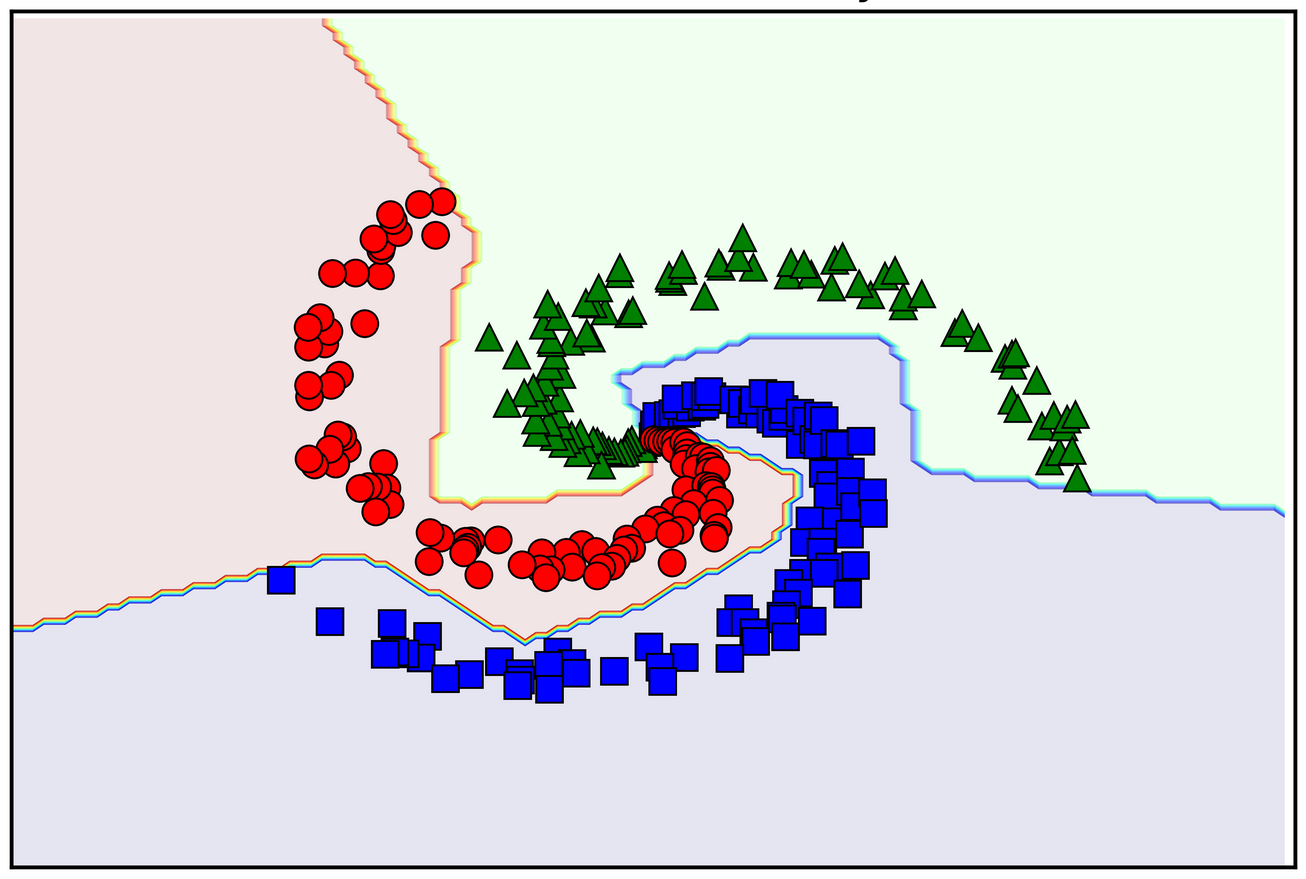
\includegraphics[width=10cm]{images/nonlinearland.PNG}
\caption{Phân lớp các dữ liệu sử dụng những miền phi tuyến tính \cite{mlpvuhuutiep}.}
\label{fig:nonlinearland}
\end{figure}

Theo như \ref{eqn:tohopcuax} thì đầu ra của tầng ẩn thứ 2 vẫn chỉ là một tổ hợp tuyến tính của $\mathbf{x}$ ban đầu.
Thế thì khi một mạng nơ-ron sâu có tất cả các tầng ẩn đều sử dụng những hàm kích hoạt tuyến tính, ta có thể rút gọn những tầng ẩn này đi mà chỉ có tầng đầu vào và tầng đầu ra.
Điều này làm cho mô hình không thể hiện được tính sâu, thứ làm nên sức mạnh của những mạng nơ-ron.
\vspace{5pt}

Ở một góc nhìn đơn giản, bản thân những hàm tuyến tính chỉ có thể làm việc được với những bài toán đơn giản.
Nếu chỉ sử dụng những hàm kích hoạt tuyến tính thì ta cũng chỉ có thể đa ra một lời giải đơn giản.
Mà rõ ràng, những bài toán được áp dụng trong mạng học sâu không chỉ có những bài toán đơn giản mà còn là những bài toán rất phức tạp.
Những hàm tuyến tính không thể nào đáp ứng được nhu cầu bài toán đưa ra, chẳng hạn như hình \ref{fig:nonlinearland}, nếu chỉ dùng những hàm tuyến tính để phân lớp thì ta sẽ không bao giờ có một lời giải tốt.
Do đó, hàm kích hoạt được yêu cầu phải là một hàm phi tuyến.
\vspace{5pt}

Nền móng của mạng nơ-ron sâu là mô hình perceptron \cite{luocsudlvuhuutiep}, với hàm kích hoạt được sử dụng là hàm dấu.
\begin{align}
    \text{sgn}(x) = \begin{cases}-1, &x < 0\\ 0, &x = 0\\ 1, &x > 0\end{cases}
\end{align}

Dù rằng là hàm này phi tuyến, nhưng thực tế lại không được sử dụng, vì đạo hàm tại hầu hết các điểm bằng 0 (trừ tại gốc toạ độ không có đạo hàm).
Việc đạo hàm bằng 0 này khiến cho các thuật toán dựa trên gradient không hoạt động.
Trong khi việc tối ưu các mạng học sâu sử dụng lan truyền ngược lại dựa trên gradient.

\section{Hàm Sigmoid và hàm Tanh}\label{sec:hamsigmoidvahamtanh}

Hàm Sigmoid, hay còn biết đến với cái tên là hàm logistic. Hàm được định nghĩa toán học như sau:
\begin{align}
    \text{Sigmoid}(x) = \sigma(x) = \dfrac{1}{1 + e^{-x}}
\end{align}

\begin{figure}[!h]
\captionsetup{width=0.8\textwidth}
\centering
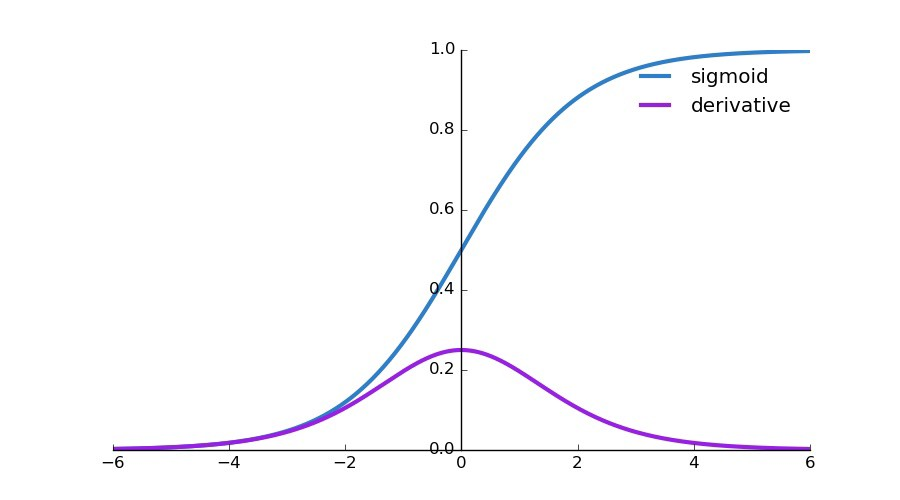
\includegraphics[width=15cm]{images/sigmoidfunc.jpg}
\caption{Đồ thị hàm số của hàm Sigmoid và đạo hàm của nó.}
\label{fig:sigmoidfunc}
\end{figure}

Nhìn vào \ref{fig:sigmoidfunc} ta thầy rằng: nếu đầu vào lớn, hàm số sẽ cho đầu ra gần với 1;
nếu đầu vào nhỏ (rất âm), hàm số sẽ cho đầu ra gần với 0.
Trước đây, hàm kích hoạt này được sử dụng rất nhiều vì có đạo hàm rất đẹp (xem hình \ref{fig:sigmoidfunc}).
Nhưng những năm gần đây, hàm số này ít khi được sử dụng để làm hàm kích hoạt cho các tầng ẩn.
Thay vào đó, hàm Sigmoi được sử dụng ở tầng đầu ra khi đầu ra là các giá trị nhị phân hoặc biểu diễn các xác suất.
\vspace{5pt}

Một hàm tương tự thường sử dụng và mang lại hiệu quả tốt hơn chính là hàm Tanh:
\begin{align}
    \tanh{x} = \dfrac{e^x - e^{-x}}{e^x + e^{-x}}
\end{align}

Hàm số này có tính chất đầu ra chạy từ -1 đến 1, khiến cho nó có tính chất tâm 0 thay vì chỉ dương như hàm Sigmoid (xem hình \ref{fig:tanhfunc}).
Tính chất tâm 0 này giúp cho mô hình có thể làm việc hiệu quả được với những tập dữ liệu chưa được chuẩn hoá tốt \cite{zerocenteredstat}.
\vspace{5pt}

\begin{figure}[!h]
\captionsetup{width=0.8\textwidth}
\centering
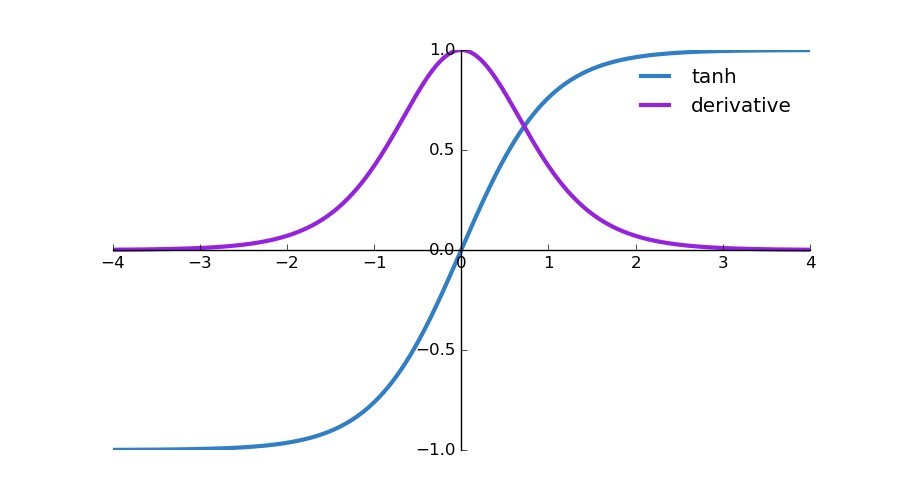
\includegraphics[width=15cm]{images/tanhfunc.jpg}
\caption{Đồ thị hàm số của hàm Tanh và đạo hàm của nó.}
\label{fig:tanhfunc}
\end{figure}

Một nhược điểm dễ nhận thấy là khi đầu vào có trị tuyệt đối lớn, đạo hàm của cả Sigmoid và Tanh tại điểm giá trị đó rất gần với 0.
Điều này đồng nghĩa với việc các hệ số tương ứng với đơn vị ẩn đang xét sẽ gần như không được thay đổi khi sử dụng công thức cập nhật theo thuật toán gradient khi tiến hành lan truyền ngược.
Hiện tượng này được gọi là hiện tượng biến mất gradient.

\section{Hàm ReLU (Rectified Linear Unit)}\label{sec:hamrelu}

Đây là hàm \cite{reluhinton} được sử dụng rộng rãi nhất trong các mô hình học sâu vì tính đơn giản của nó (xem hình \ref{fig:relufunc}).
Tuy đơn giản, nhưng không hề đồng nghĩa với ít hiệu quả.
Hàm kích hoạt này có công thức toán học là:
\begin{align}
    \text{ReLU}(x) = \mathcal{R}(x) = \max\left(0, x\right)
\end{align}

Một cách nôm na, ta có thể miêu tả hàm ReLU như sau:
\begin{itemize}
    \item Nếu đầu vào nhỏ hơn hoặc bằng 0, thì đầu ra là 0.
    \item Nếu đầu vào lớn hơn 0, thì đầu ra là chính nó, tức đầu ra đúng bằng đầu vào.
\end{itemize}

\begin{figure}[!h]
\captionsetup{width=0.8\textwidth}
\centering
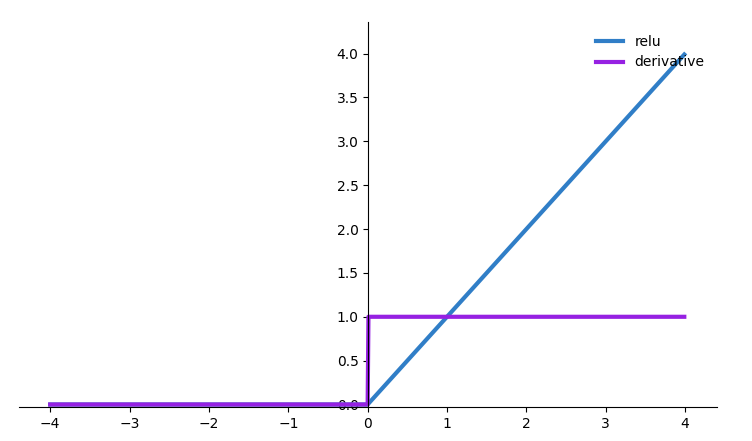
\includegraphics[width=15cm]{images/relufunc.PNG}
\caption{Đồ thị hàm số của hàm ReLU và đạo hàm của nó.}
\label{fig:relufunc}
\end{figure}

Ta có thể thấy, hàm ReLU thực sự rất đơn giản trong tính toán.
Nhìn vào tưởng chừng không khác mấy so với một hàm tuyến tính thông thường.
Hay thay, điều đơn giản này lại khắc phục được hiện tượng biến mất gradient mà hàm Sigmoid và Tanh mắc phải.
Để có thể thấy rõ điều đó, ta sẽ xem xét đạo hàm của hàm ReLU.
Hiển nhiên, ta không khó để ta tính được:
\begin{align}
    \dfrac{\text{d}\mathcal{R}}{\text{d}x} = \max\left(\text{sgn}\left(x\right)\right) = \begin{cases}1, x > 0\\0, x \le 0\end{cases}
\end{align}

Cũng như chính hàm ReLU, đạo hàm của nó cũng hết sức đơn giản:
\begin{itemize}
    \item Nếu đầu vào nhỏ hơn hoặc bằng 0, thì đầu ra là 0.
    \item Nếu đầu vào lớn hơn 0, thì đầu ra là 1.
\end{itemize}

Vậy nên sẽ không xuất hiện chuyện khi đầu vào quá lớn, đạo hàm tại giá trị đó sẽ rất gần 0, khiến cho việc cập nhật giá trị tham số mô hình diễn ra chậm.
ReLU được chứng minh là đã giúp việc huấn luyện mạng nơ-ron đa tầng nhanh hơn rất nhiều so với lại hàm Tanh.
\vspace{5pt}

Nhưng hàm này lại gây ra một trở ngại khác, chính là chết ReLU.
Mọi đầu vào nhỏ hơn hoặc bằng 0 đều sẽ được đưa về 0.
Chuyện gì sẽ xảy ra khi ta có nhiều đầu vào nhỏ hơn 0?
Hiển nhiên là kết quả tệ và thậm chí là tệ hơn so với biến mất gradient, khi giá trị tham số sẽ không có cách nào thay đổi và mãi như vậy do đạo hàm của những giá trị đầu vào này đều là giá trị 0.
Một số chứng minh thực nghiệm cho thấy, việc này có thể được khắc phục bằng cách tăng số lượng đơn vị ẩn \cite{activationfunctionandrew}.
Tuy nhiên, việc này cần phải cẩn thận khi Lu Lu \cite{Lu_2020} đã chứng minh lý thuyết được rằng một mạng học sâu với hàm kích hoạt ReLU sẽ chết khi độ sâu lên đến vô hạn.
\vspace{5pt}

Ưu điểm dễ dàng nhận ra của RELU đó chính là việc tính toán đơn giản, giúp cho chi phí tính toán sẽ đơn giản hơn những hàm sử dụng hàm mũ.
Đồng thời hàm này cũng khắc phục được hiện tượng biến mất gradient.
Tuy thế, phần âm đưa hết về 0 của hàm lại gây nên hiện tượng chết ReLU.

Theo kinh nghiệm của những kỹ sư đi trước, khi xây dựng một mạng nơ-ron đa tầng, hàm kích hoạt ReLU nên được thử đầu tiên, vì nó nhanh cho kết quả và thường hiệu quả trong nhiều trường hợp.

\section{Hàm Leaky ReLU}\label{sec:hamleakyrelu}

Đây là một biến thể của ReLU \cite{leakyandrew} mà có khả năng khắc phục hiện hượng chết ReLU.
Công thức toán học miêu tả hàm này như sau:
\begin{align}
    \text{Leaky ReLU}(x) = \mathcal{R}_L(x) = \begin{cases}x, &x > 0\\\alpha x, &x \le 0\end{cases}; \alpha \in \left(0, 1\right)
\end{align}

\begin{figure}[!h]
\captionsetup{width=0.8\textwidth}
\centering
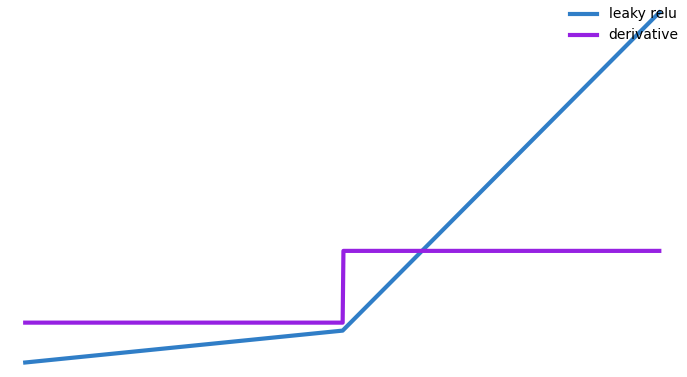
\includegraphics[width=15cm]{images/lrelu.PNG}
\caption{Đồ thị hàm số của hàm Leaky ReLU ($\alpha = 0.1$) và đạo hàm của nó.}
\label{fig:lrelu}
\end{figure}

Nửa khoảng giá trị $\left(0, +\infty\right)$, hai hàm ReLU và Leaky ReLU hoàn toàn giống nhau.
Duy chỉ phần nửa đoạn $\left(-\infty, 0\right]$, hàm Leaky ReLU đã có một chút sự thay đổi thay vì chỉ là giá trị 0 như ReLU.
Bây giờ, những giá trị âm sẽ có giá trị là $\alpha x$ thay vì giá trị $0$.
Đạo hàm của Leaky ReLU cũng vì thế mà sẽ là:
\begin{align}
    \dfrac{\text{d}\mathcal{R}_L}{\text{d}x} =  \begin{cases}1, x > 0\\\alpha, x \le 0\end{cases}
\end{align}

Nhờ như vậy, những đầu vào nhỏ hơn 0 bây giờ sẽ không bị đưa hết về 0 mà sẽ là $\alpha$.
Điều này có nghĩa là, hiện tượng chết ReLU đã được xử lý.
\vspace{5pt}

Việc lựa chọn giá trị $\alpha$ cho thực sự hiệu quả cũng là một vấn đề không hề đươn giản.
Nếu giá trị $\alpha = 0$, Leaky ReLU chính là ReLU.
Còn nếu $\alpha = 1$, thì Leaky ReLU sẽ trở thành một hàm tuyến tính, nên không ai sử dụng Leaky ReLU với $\alpha = 1$.
Thông thường, $\alpha$ sẽ được chọn là 0.01, tức 1 phần 100.
Cũng có một số mô hình chọn giá trị $\alpha$ lớn hơn một chút, khoảng từ 0.1 tới 0.3.
Đã có nhiều cải thiện được đề xuất cho Leaky ReLU và cũng đã có những kết quả khả quan trên một số thực nghiệm.
Có thể liệt kê qua như việc học hệ số $\alpha$ này trong quá trình huấn luyện với hàm đề xuất là PReLU (Parametric Rectified Linear Unit).
Hoặc là ngẫu nhiên chọn hệ số $\alpha$ dựa vào một biến ngẫu nhiên theo một phân phối đều - RReLU (Randomized Leaky Rectified Linear Unit).
\vspace{5pt}

Có thể nói, Leaky ReLU đã thừa hưởng được những đặc điểm tốt của ReLU, ngoài ra còn khắc phục được hiện tượng chết ReLU của phiên bàn gốc.
Nhưng một điều khá rắc rối là việc chọn hệ số $\alpha$ cần phải được thực hiện một cách hợp lý, hoặc phải dùng thuật toán học, nếu không dễ gây tác dụng không đáng có.

\section{Hàm ELU (Exponential Linear Unit)}\label{sec:hamelu}

Cũng như Leaky ReLU, hàm ELU \cite{clevert2016fast} được đưa ra để khắc phục điểm yếu của ReLU.
Một hệ số $\alpha$ sẽ được chọn giống như cách chọn cho hàm Leaky ReLU, đôi khi sẽ là chọn bằng kinh nghiệm, và có lúc sẽ là học trong quá trình huấn luyện.
Nhưng ELU không còn giữ được tính đơn giản tính toán như Leaky ReLU hay ReLU tuy hình dáng không thay đổi nhiều (xem hình \ref{fig:elufunc}).
Công thức toán học của ELU có thể được biểu diễn như sau:
\begin{align}
    \text{ELU}(x) = \mathcal{E}(x) = \begin{cases}x, &x > 0\\\alpha\left(e^x - 1\right), &x \le 0\end{cases}; \alpha \in \left(0, 1\right)
\end{align}

Nếu đầu vào lớn hơn 0, đầu ra bằng đúng đầu vào.
Còn với những đầu vào bé hơn hoặc bằng 0, chúng ta sẽ có một giá trị chỉ là gần với 0.
Khác so với ReLU, khi ReLU sẽ đưa hết tất cả về 0.
Leaky ReLU thì sẽ đưa trị tuyệt đối của giá trị đó nhỏ lại theo hệ số $\alpha$.
Những thay đổi của ELU cũng không làm mất đi tính chất của những họ hàm LU, dùng để giải quyết biến mất gradient.
Nếu như vậy, thì ELU có tránh được việc chết ReLU như Leaky ReLU làm được?
Ta hãy cùng xem đạo hàm của ELU:
\begin{align}
    \dfrac{\text{d}\mathcal{E}}{\text{d}x} =  \begin{cases}1, &x > 0\\\alpha e^x, &x \le 0\end{cases} =  \begin{cases}1, &x > 0\\\alpha\left(e^x - 1\right) + \alpha, &x \le 0\end{cases} =  \begin{cases}1, &x > 0\\\mathcal{E}(x) + \alpha, &x \le 0\end{cases}\label{eqn:daohamelu}
\end{align}

Lý do ta nên biểu diễn đạo hàm phía âm của hàm ELU dưới dạng $\mathcal{E}(x) + \alpha$ thay vì $\alpha e^x$ (\ref{eqn:daohamelu}) là để tái sử dụng lại giá trị $\mathcal{E}(x)$ thay vì phải tính lại giá trị $e^x$.
\vspace{5pt}

\begin{figure}[!h]
\captionsetup{width=0.8\textwidth}
\centering
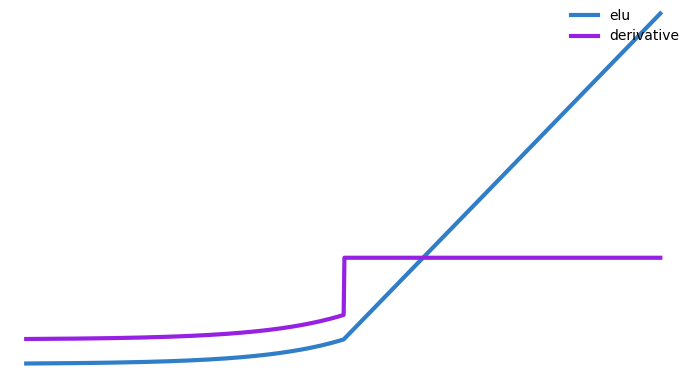
\includegraphics[width=15cm]{images/elufunc.PNG}
\caption{Đồ thị hàm số của hàm ELU ($\alpha = 0.3$) và đạo hàm của nó.}
\label{fig:elufunc}
\end{figure}

Trở lại với việc rằng liệu ELU có tránh được việc chết ReLU hay không, ta cần chú ý vào phần phía âm, tức đại lượng $\mathcal{E}(x) + \alpha$.
Rõ ràng rằng dù đầu vào của $\mathcal{E}(x)$ có âm như thế nào, thì giá trị nhận về cũng là một số âm gần với 0.
Khi cộng với một $\alpha$ lớn vừa phải, giá trị này sẽ có xu hướng lớn hơn 0 một tí, vừa đủ để thoát khỏi được hiện tượng chết ReLU.
Khác với Leaky ReLU, hàm ELU vẫn có thể có một vài đơn vị ẩn bị chết, tức không cập nhật được tham số nếu đầu vào rất âm.
Vì khi đó $\mathcal{E}(x)$ không còn quá gần 0, khi cộng vào với $\alpha$, sẽ có xu hướng rất sát với 0 như Sigmoid hoặc Tanh.
Hoặc có thể hiểu là do việc $x \rightarrow -\infty$ sẽ suy ra được $e^x \rightarrow 0$.
\vspace{5pt}

Hàm ELU cũng có được những ưu điểm của Leaky ReLU, tuy vậy việc tính toán lúc này sẽ phức tạp hơn một chút vì có đại lưỡng mũ.

\section{Hàm SELU (Scaled Exponential Linear Unit)}\label{sec:hamselu}

Hàm này \cite{klambauer2017selfnormalizing} là một trong những hàm khá mới (xem hình \ref{fig:selufunc}).
Việc cài đặt hàm này để sử dụng trong thực tiễn một cách hiệu quả cũng cần phải có nhiều công sức hơn so với các hàm đã giới thiệu.
Theo hướng dẫn, các trọng số cũng như bias của mạng cần phải được khởi tạo với LeCun Normal \cite{activationcasper}.
Trong trường hợp mạng có sử dụng kỹ thuật dropout, thì cần phải sử dụng Alpha Dropout.
Tác giả khi đề xuất hàm này, đã tính toán 2 giá trị quan trọng cho hàm này, chính là $\alpha$ và $\lambda$:
\begin{align}
    \alpha \approx 1.6732632423543772848170429916717 \label{eqn:selualpha}\\
    \lambda \approx 1.0507009873554804934193349852946 \label{eqn:selulambda}
\end{align}

Không giống như Leaky ReLU hay ELU, đây là những giá trị đã được các tác giả tính toán trước và áp dụng cho mọi mô hình.
Giống như cái tên của mình, đây là một hàm tỷ lệ với hàm ELU, chính xác là tỷ lệ với hệ số $\lambda$ (\ref{eqn:selulambda}):
\begin{align}
    \text{SELU}(x) = \mathcal{E}_S(x) = \lambda \begin{cases}x, &x > 0\\\alpha\left(e^x - 1\right), &x \le 0\end{cases}
\end{align}

Đạo hàm của SELU cũng không khác ELU là bao:
\begin{align}
    \dfrac{\text{d}\mathcal{E}_S}{\text{d}x} =  \lambda\dfrac{\text{d}\mathcal{E}}{\text{d}x} =  \begin{cases}1, &x > 0\\\mathcal{E}_S(x) + \alpha, &x \le 0\end{cases}\label{eqn:daohamselu}
\end{align}

\begin{figure}[!h]
\captionsetup{width=0.8\textwidth}
\centering
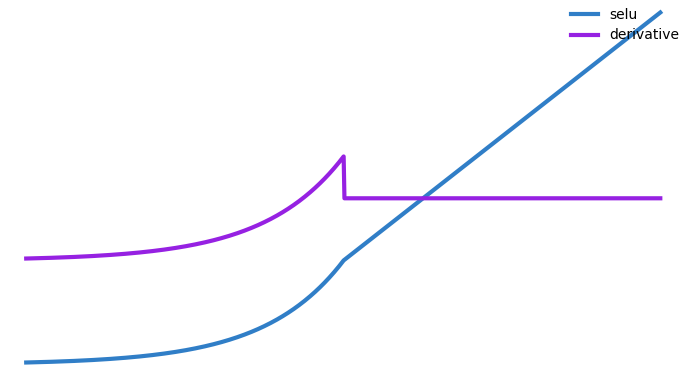
\includegraphics[width=15cm]{images/selufunc.PNG}
\caption{Đồ thị hàm số của hàm SELU và đạo hàm của nó.}
\label{fig:selufunc}
\end{figure}

Bây giờ, nếu đầu vào lớn hơn 0 thì giá trị đầu ra cần phải tỷ lệ theo một hệ số $\lambda$ thành là $\lambda x$ hay vì chính bằng $x$.
Phần miền nhỏ hơn hoặc bằng 0, tương tự một hàm ELU với giá trị $\alpha$ (\ref{eqn:selualpha}) đã chọn nhưng giá trị sẽ được tỷ lệ với $\lambda$.
\vspace{5pt}

Chọn một số $\alpha$ để cài đặt cho hàm ELU, và tỷ lệ với một hằng số $\lambda$, điều gì khiến hàm này trở nên đặc biệt?
Lý thuyết mà nói, hàm SELU là hàm có khả năng tự chuẩn hoá đầu ra nếu được cài đặt đúng như những gì đã yêu cầu.
Thay vì phải thêm một tầng chuẩn hoá đầu ra như một số các hàm khác, thì khi sử dụng SELU, bước chuẩn hoá này đã được hàm SELU tự động hoàn thành trong nội bộ.
Điều này giúp giảm thời gian huấn luyện của mô hình sử dụng hàm SELU.
\vspace{5pt}

Về bản chất, SELU cũng vẫn là một dạng tỷ lệ của ELU, nên cách nó khắc phục biến mất gradient và chết ReLU không khác gì ELU.
Nếu đúng như lý thuyết, thì SELU lợi thế hơn ELU ở điểm có khả năng tự chuẩn hoá, bớt cồng kềnh cho mạng sử dụng.

\section{Hàm GELU (Gaussian Error Linear Unit)}\label{sec:hamgelu}

Được sử dụng nhiều gần đây trong kiến trúc Transformers - Google's BERT và OpenAI's GPT-2.
Tuy ra đời cũng không phải là quá mới, khi 2016 đã được trình làng \cite{hendrycks2020gaussian}, nhưng mãi ít năm gần đây mới được chú ý tới.
Mô tả toán học của hàm này như sau:
\begin{align}
    \text{GELU}(x) = \mathcal{G}(x) = 0.5x\left\{1 + \tanh\left[\sqrt{\dfrac{2}{\pi}}\left(x + 0.044715x^3\right)\right]\right\}
\end{align}

\begin{figure}[!h]
\captionsetup{width=0.8\textwidth}
\centering
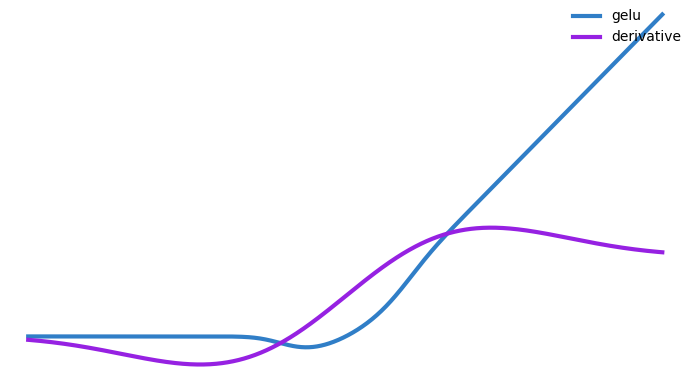
\includegraphics[width=15cm]{images/gelu.PNG}
\caption{Đồ thị hàm số của hàm GELU và đạo hàm của nó.}
\label{fig:gelufunc}
\end{figure}

Không có gì là giống với những hàm LU trước, khi bây giờ GELU là tổ hợp của nhiều hàm cộng lại: hàm Tanh, hàm đa thức, những hệ số vô tỉ.
Nếu để ý kĩ, hàm Tanh sẽ cho giá trị gần với 1 khi $x$ dương lớn, như vậy hàm GELU sẽ có giá trị đầu ra đúng gần bằng với đầu vào như là một hàm Linear Unit.
Muốn có cái nhìn chính xác của điều trên, ta quan sát những giá trị giới hạn và phép tương đương sau:
\begin{align}
\lim_{x \rightarrow +\infty}&\sqrt{\dfrac{2}{\pi}}\left(x + 0.044715x^3\right) = +\infty\\
\lim_{x \rightarrow +\infty}&0.5\left(1 + \tanh(x)\right) = 0.5\left(1 + 1\right) = 1\\
\mathcal{G}(x) \sim & 0.5x\left(1 + 1\right) = x, x \rightarrow +\infty
\end{align}

Trường hợp $x$ âm lớn, hàm Tanh sẽ cho ta giá trị gần với -1 khiến cho kết quả của hàm GELU có giá trị gần với 0.
Đại lượng âm vô cùng $x$ sẽ được khử với giá trị 0 của 1 + hàm Tanh.
Để hiểu rõ chỗ này, ta cần một số kiến thức giải tích cơ bản về chuỗi xấp xỉ tương đương Taylor-Maclaurin:
\begin{align}
    \frac{1}{1+x} = \sum_{n=0}^{\infty}(-1)^nx^n = 1 - x + x^2 - x^3 + \dots
\end{align}

Từ đó, ta có thể tương đương hàm Tanh như sau:
\begin{align}
    \tanh(x) &= \frac{e^x - e^{-x}}{e^x + e^{-x}} = \left(e^{2x} - 1\right).\dfrac{1}{e^{2x} + 1}\nonumber\\
    &= \left(e^{2x} - 1\right)\left(1 - e^{2x} + \dots\right) \sim -1 + e^{2x}, x \rightarrow -\infty \label{eqn:maclaurinoftanh}
\end{align}

Dựa vào \ref{eqn:maclaurinoftanh} vừa khai triển, ta suy ra được:
\begin{align}
    \tanh\left[\sqrt{\dfrac{2}{\pi}}\left(x + 0.044715x^3\right)\right] \sim \tanh\left(kx^3\right) \sim -1 + e^{2kx^3}, x \rightarrow -\infty
\end{align}

Theo đó, ta sẽ có được kết quả giới hạn:
\begin{align}
    \lim_{x \rightarrow -\infty}\mathcal{G}(x) &= \lim_{x \rightarrow -\infty}0.5x\left\{1 + \tanh\left[\sqrt{\dfrac{2}{\pi}}\left(x + 0.044715x^3\right)\right]\right\} \nonumber\\
    &= \lim_{x \rightarrow -\infty}0.5x\left\{1 - 1 + e^{2kx^3}\right\} \nonumber\\
    &= \lim_{x \rightarrow -\infty}0.5xe^{2kx^3} \nonumber\\
    &= \lim_{x \rightarrow +\infty}-\dfrac{0.5x}{e^{2kx^3}}; e^{x} >> x, x \rightarrow +\infty \nonumber\\
    &= 0
\end{align}

Không quá gian nan để tìm ra đạo hàm của GELU, bằng đạo hàm của hàm hợp ta có:
\begin{align}
     \dfrac{\text{d}\mathcal{G}}{\text{d}x} = 0.5&\tanh\left(0.0356774x^3 + 0.797885x\right) \nonumber\\
     &+ \frac{0.0535161x^3+ 0.398942x}{\cosh^2\left(0.0356774x^3 + 0.797885x\right)} + 0.5
\end{align}

Trong đó, hàm Cosh được định nghĩa như sau:
\begin{align}
    \cosh(x) = \dfrac{e^x + e^{-x}}{2}    
\end{align}

Cosh là một vô cùng lớn khi $x \rightarrow \infty$, nên là:
\begin{align}
    \lim_{x \rightarrow \infty}\dfrac{x^3}{\cosh(x^3)} &= 0\\
    \Rightarrow \dfrac{\text{d}\mathcal{G}}{\text{d}x} \sim 0.5\tanh(x^3) + 0.5 &\sim 0.5 + 0.5 = 1, x \rightarrow +\infty\\
    \Rightarrow \dfrac{\text{d}\mathcal{G}}{\text{d}x} \sim 0.5\tanh(x^3) + 0.5 &\sim -0.5 + 0.5 = 0, x \rightarrow -\infty
\end{align}

Nhìn sơ qua thì có vẻ công thức của GELU và đạo hàm của nó khá phức tạp, tuy nhiên khi được biểu diễn đồ thị lại là có hình ảnh cong mượt mà khá đẹp (xem hình \ref{fig:gelufunc}).
Điều này khác với những ReLU, Leaky ReLU, ELU hay SELU khi đồ thị hàm số bị gãy và đạo hàm không được liên tục (đạo hàm của ELU chỉ liên tục khi và chỉ khi $\alpha = 1$).
\vspace{5pt}

Tuy đã được đề xuất từ lâu, nhưng cũng như SELU, nghiên cứu về hiệu xuất hàm này trong thực tiễn vẫn chưa nhiều nên cần nhiều thực nghiểm để đưa ra kiểm chứng.

\section{Hàm Swish}\label{sec:hamswish}

\begin{figure}[!h]
\captionsetup{width=0.8\textwidth}
\centering
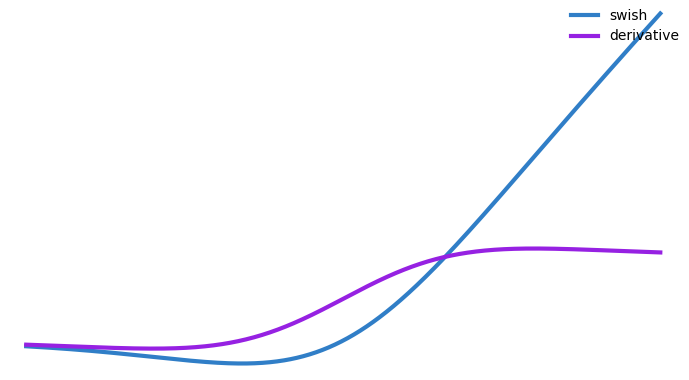
\includegraphics[width=15cm]{images/swish.PNG}
\caption{Đồ thị hàm số của hàm Swish ($\beta = 1$) và đạo hàm của nó.}
\label{fig:swishfunc}
\end{figure}

Không kinh khủng như GELU, Swish \cite{ramachandran2017searching} có công thức đơn giản hơn khi là một hàm tuyến tính bội với một hàm Sigmoid.
Đó cũng là lí do mà hàm này còn có cái tên khác là SiLU (Sigmoid Linear Unit):
\begin{align}
    \text{Swish}(x) = \mathcal{S}(x) = x\sigma(\beta x) = \dfrac{x}{1 + e^{-\beta x}}; \beta \in \mathbb{R}
\end{align}

Giống với các hàm LU khác (trừ Leaky ReLU), Swish không bị chặn trên nhưng lại bị chặn dưới.
Swish có hình dạng khá giống với GELU khi nó rất mượt mà không gãy và trông còn có vẻ mượt hơn (Xem hình \ref{fig:swishfunc}).
\vspace{5pt}

Có 2 trường hợp đặc biệt của hệ số $\beta$.
Với $\beta$ được chọn là $0$, hàm Swish gần giống như một hàm tuyến tính vì $\sigma(0x) = 0.5$.
Nếu $\beta \rightarrow \infty$, hàm Swish giờ đây trở thành một hàm ReLU do $\displaystyle \lim_{\beta \rightarrow -\infty}\sigma(\beta x) = 0, \lim_{\beta \rightarrow +\infty}\sigma(\beta x) = 1$.
Swish nằm giữa 2 thái cực là tuyến tính và ReLU biến thiên nhờ vào hệ số $\beta$.
\vspace{5pt}

Đạo hàm của hàm Swish tính được theo đạo hàm hàm hợp như sau:
\begin{align}
    \dfrac{\text{d}\mathcal{S}}{\text{d}x} &= \sigma\left(\beta x\right) + x.\beta\sigma\left(\beta x\right)\left(1 - \sigma\left(\beta x\right)\right) \nonumber\\
    &= \sigma\left(\beta x\right) + \beta x\sigma\left(\beta x\right) - \beta x \sigma^2\left(\beta x\right) \nonumber\\
    &= \beta x\sigma\left(\beta x\right) + \sigma\left(\beta x\right) - \beta x \sigma^2\left(\beta x\right) \nonumber\\
    &= \beta \mathcal{S}(x) + \sigma\left(\beta x\right)\left(1 - \beta \mathcal{S}(x)\right)
\end{align}

Đạo hàm của Swish có hình dáng gần giống với GELU và liên tục trên toàn miền (Xem hình \ref{fig:swishfunc}).
Về mặt lý thuyết, có vẻ Swish khá tương tự với GELU và cũng chưa có nhiều thực nghiệm trên các mô hình khác nhau của hàm này nên cũng chưa thể đưa ra nhận xét nào quá đặc biệt.

\section{Thông tin về các hàm kích hoạt được thực nghiệm}\label{sec:thongtincachamthucnghiem}

Trong các phần thực nghiệm sau, những hàm được đem vào những mô hình để đánh giá là Sigmoid, Tanh ($\tanh$), ReLU ($\mathcal{R}$), Leaky ReLU - sẽ được gọi tắt là Leaky ($\mathcal{R}_L (\alpha = 0.2)$), ELU ($\mathcal{E} (\alpha = 1)$), SELU ($\mathcal{E}_S = \lambda \mathcal{E}$), GELU ($\mathcal{G}$) và cuối cùng là Swish ($\mathcal{S} (\alpha = 1)$).

%%%%%%%%%%%%%%%%%%%%%%%%%%%%%%
\chapter{Thực nghiệm so sánh trên tập dữ liệu MNIST}\label{chap:thucnghiemmnist}

Thực nghiệm đầu tiên sẽ là trên tập dữ liệu MNIST\footnote{THE MNIST DATABASE of handwritten digits, đường dẫn: \href{http://yann.lecun.com/exdb/mnist/}{http://yann.lecun.com/exdb/mnist/}}, xem xem những hàm kích hoạt khác nhau sẽ hoạt động thế nào  trong bài toán phân loại chữ số viết tay từ 0 tới 9.
Tập dữ liệu gồm 60,000 ảnh huấn luyện và 10,000 ảnh kiểm tra.
Mỗi ảnh là một ảnh xám có kích thước $28 \times 28 \times 1$, có điểm ảnh có giá trị ban đầu cao nhất là 255 và thấp nhất là 0, sau được chuẩn hoá lại về khoảng giá trị $[0, 1]$ bằng cách chia giá trị tất cả các điểm ảnh cho 255.
Trong quá trình huấn luyện, không sử dụng bất cứ kỹ thuật làm giàu dữ liệu nào.
Một lưu ý là, tập ảnh dữ liệu kiểm tra sẽ được dùng để kiểm định trong quá trình huấn luyện, tức ta sẽ bỏ qua quá trình kiểm tra và ta có thể xem như giá trị kiểm định cuối cùng là giá trị kiểm tra nếu muốn.
\vspace{5pt}

Các thông số của mạng như chiều sâu của mạng, kiểu khởi tạo trọng số, kích thước batch, tốc độ học, và thuật toán tối ưu đều có một ảnh hưởng nhất định lên quá trình huấn luyện một mô hình mạng học sâu.
Một số ảnh hưởng được đưa ra thử nghiệm để đánh giá như là việc tăng độ sâu của một mạng nơ-ron, thay đổi cách khởi tạo trọng số, thêm nhiễu vào dữ liệu, sử dụng kiến trúc mạng tích chập.
Đối với việc tăng độ sâu của mạng, kỹ thuật của mạng dư thừa không được áp dụng do cách thức trên sinh ra để xử lý việc tăng độ sâu của mạng, phần nào giảm đi tính đúng đắn về hiệu quả của các hàm kích hoạt.

\section{Thực nghiệm thông qua mạng nơ-ron sâu}\label{sec:mnistdl}

Bao gồm 11 kiến trúc được đưa ra, mỗi kiến trúc có số lượng tầng ẩn lần lượt tăng từ 2 cho tới 12.
Mỗi ảnh đầu vào sẽ được làm phẳng thành một vector có số chiều 728 (chính là $28 \times 28 \times 1 = 728$) tương ứng với số đơn vị ở tầng đầu vào.
Tầng đầu ra sẽ là 10 đơn vị ẩn tương ứng với 10 lớp từ 0 tới 9.
Các tầng ẩn sẽ có số lượng đơn vị ẩn như sau:

\begin{itemize}
    \item 2 tầng ẩn: $512 \rightarrow 128$.
    \item 3 tầng ẩn: $512 \rightarrow 256 \rightarrow 128$.
    \item 4 tầng ẩn: $512 \rightarrow 256 \rightarrow 128 \rightarrow 64$.
    \item 5 tầng ẩn: $512 \rightarrow 256 \rightarrow 128 \rightarrow 64 \rightarrow 32$.
    \item 6 tầng ẩn: $512 \rightarrow 256 \rightarrow 128 \rightarrow 64 \rightarrow 32 \rightarrow 16$.
    \item 7 tầng ẩn: $512(\times 2) \rightarrow 256 \rightarrow 128 \rightarrow 64 \rightarrow 32 \rightarrow 16$.
    \item 8 tầng ẩn: $512(\times 2) \rightarrow 256(\times 2) \rightarrow 128 \rightarrow 64 \rightarrow 32 \rightarrow 16$.
    \item 9 tầng ẩn: $512(\times 2) \rightarrow 256(\times 2) \rightarrow 128(\times 2) \rightarrow 64 \rightarrow 32 \rightarrow 16$.
    \item 10 tầng ẩn: $512(\times 2) \rightarrow 256(\times 2) \rightarrow 128(\times 2) \rightarrow 64(\times 2) \rightarrow 32 \rightarrow 16$.
    \item 11 tầng ẩn: $512(\times 2) \rightarrow 256(\times 2) \rightarrow 128(\times 2) \rightarrow 64(\times 2) \rightarrow 32(\times 2) \rightarrow 16$.
    \item 12 tầng ẩn: $512(\times 2) \rightarrow 256(\times 2) \rightarrow 128(\times 2) \rightarrow 64(\times 2) \rightarrow 32(\times 2) \rightarrow 16(\times 2)$.
\end{itemize}

Sau mỗi tầng dày đặc, một dropout có tỷ lệ 50\% sẽ được áp dụng, riêng với tầng ẩn cuối cùng của mỗi kiến trúc, tỷ lệ dropout giảm xuống 25\%.
\vspace{5pt}

Khi huấn luyện các mô hình với những hàm kích hoạt khác nhau, để cho công bằng thì khi cài đặt đều sử dụng chung một hàm tối ưu, tốc độ học và cùng một kiểu khởi tạo trọng số.
Kỹ thuật dropout cũng sẽ giống nhau nếu không có lưu ý gì.

\subsection{Dữ liệu không nhiễu và khởi tạo trọng số theo chuẩn hoá Lecun}\label{subsec:mnistd}

Tất cả được khởi tạo trọng số theo chuẩn hoá Lecun, riêng đối với mô hình áp dụng hàm kích hoạt SELU sẽ sử dụng kỹ thuật alpha dropout với tỷ lệ bằng với tỷ lệ dropout của các hàm kích hoạt khác.
Biểu đồ giá trị chính xác và mất mát trên tập kiểm định qua mỗi epoch được cho ở các hình \ref{fig:mnistd1}, \ref{fig:mnistd2}, \ref{fig:mnistd3}, \ref{fig:mnistd4}.
Chi tiết về giá trị được cho ở bảng \ref{tab:mnistdacc} và bảng \ref{tab:mnistdloss}.
Ở phần bảng giá trị không có thống kê của Sigmoid, do hàm này có kết quả tệ khá rõ rệt (sẽ được nêu rõ ngay sau đầy).
\vspace{5pt}

Với mạng nơ-ron không quá sâu - 2 tầng ẩn (hình \ref{fig:mnistd1a}, \ref{fig:mnistd1b}), các hàm dễ dàng đạt được độ chính xác cao (tất cả đều trên 92\%) và giá trị mất mát thấp (tất cả đều dưới 0.40).
Hàm Sigmoid không được tích cực giống như các hàm còn lại khi thua thiệt hẳn về tốc độ hội tụ khi mãi gần 20 epoch mới đạt được mất mát dưới giá trị 1.
Tuy các hàm ngoài Sigmoid chưa thấy được sự khác biệt rõ rệt, nhưng có vẻ như SELU là người yếu thế nhất trong nhóm này khi giá trị mất mát tuy hội tụ khá sớm.
Chỉ sau 20 epoch (bảng \ref{tab:mnistdepoch}), 80\% giá trị mất mát đã bằng giá trị mất mát cuối cùng.
Nhưng kết quả mất mát cuối cùng không quá ấn tượng và gần bằng so với Sigmoid.
\vspace{5pt}

Ngay khi tăng lên 3 tầng ẩn (hình \ref{fig:mnistd1c}, \ref{fig:mnistd1d}), Sigmoid đã cho thấy sự lép vế rõ rệt.
Không chỉ thế, SELU cũng có vẻ sẽ chung số phận với Sigmoid khi số lượng tầng ẩn tiếp tục tăng.
Dù cho cuối cùng SELU vẫn đạt giá trị chính xác trên 92\% nhưng giá trị mất mát đã tiệm cận 0.50 (chính xác là 0.49).
\vspace{5pt}

Sigmoid chính thức bỏ cuộc khỏi cuộc đua khi tới số tầng ẩn là 5 (hình \ref{fig:mnistd2a}, \ref{fig:mnistd2b}), gần như mô hình với hàm này không thể học được.
SELU tuy vẫn còn có khả năng học, nhưng cho kết quả rất tệ như Sigmoid những mô hình ban đầu khi giá trị mất mát đạt tới 1.67.
Dù cho vẫn giữ được độ chính xác gần 90\%, nhưng khi tăng thêm số tầng ẩn thì có khả năng cao sẽ bị giảm đi thấp rất nhiều.
Ngoài ra, ta thấy rằng hàm ELU và Tanh có vẽ hội tụ nhanh hơn so với các hàm còn lại, và chính xác là như thế khi ELU chỉ cần đúng 3 epoch để 80\% mất mát hiện tại bằng mất ngưỡng.
Với Tanh thì con số này là 24 epoch.
Kế đến là Leaky và RELU ngay sau (cùng 27 epoch), Swish (38) và GELU (35) ở nhóm sau cùng.
Giá trị chính xác và mất mát của các hàm kích hoạt sau 50 epoch vẫn chưa có sự chênh lệch đáng kể.
\vspace{5pt}

Độ sâu được nâng lên 7 tầng ẩn (hình \ref{fig:mnistd2e}, \ref{fig:mnistd2f}), Leaky đã bỏ lại RELU chung với nhóm của GELU và Swish ở khoảng 15 epoch đầu tiên.
Mãi khi về cuối, RELU cũng như GELU và Swish mới bám được với nhóm dẫn đầu gồm có ELU, Tanh và Leaky.
Lúc này, vẫn chưa có sự chênh lệch quá đáng kể về giá trị chính xác cũng như mất mát.
Duy chỉ có Swish có vẻ đuối sức so với những hàm còn lại khi giá trị chính xác duy trì được $\approx$ 95\% giảm xuống 92.03\%.
SELU lúc này đã không còn có khả năng tiếp tục khi giá trị chính xác giảm thảm hại xuống 37.25\% và giá trị mất mát là 7.02.
So với lúc 5 tầng ẩn thì đã giá trị chính xác đã giảm đi 50\%, giá trị mất mát thì tăng lên 5.35.
\vspace{5pt}

Kết quả khi số tầng ẩn tăng lên là 9 (hình \ref{fig:mnistd3c}, \ref{fig:mnistd3d}) cho thấy chỉ có Leaky, Elu và Tanh là đủ sức để đi tiếp những mô hình sâu hơn khi vẫn giữ được giá trị chính xác trên 90\%.
Trong nhóm này, ELU có vẻ nổi trội hơn một chút so với hai hàm còn lại ở những epoch đầu.
Dẫu thế, những kết quả về cuối cho thấy ELU vẫn chưa thể tách nhóm khi giá trị chính xác vẫn chỉ đang xấp xỉ Leaky.
Nhóm còn lại gồm RELU, GELU và Swish thì chỉ có RELU và GELU tiếp tục khi Swish cũng cho thấy sự hụt hơi của mình (chính xác: 57.32\%, mất mát: 1.21).
Tuy nhiên ở ngay độ sâu kế tiếp - 10 tầng ẩn (hình \ref{fig:mnistd3e}, \ref{fig:mnistd3f}), GELU cũng như Swish đã không còn có khả năng học được nữa khi giá trị chính xác cũng như mất mát đã bão hoà ở mức 10.60\% và 2.30.
\vspace{5pt}

Ở mô hình cuối cùng - 12 tầng ẩn (hình \ref{fig:mnistd4c}, \ref{fig:mnistd4d}), Leaky lúc này cũng không còn bám được với nhóm đầu dù là những epoch cuối khi giá trị tụt xuống 62.84\% và mất mát 1.08.
Nhà vô địch ở mô hình này là ELU với chiến thắng khá thuyết phục khi ta thấy có cách biệt rõ rệt giữa ELU so với Tanh và cụ thể là giá trị chính xác 79.24\% > 76.97\%, giá trị mất mát 0.45 < 0.6.
Tốc độ hội tụ của ELU cũng nhanh hơn rõ rệt khi sau 16 epoch đã đạt được giá trị cần thiết so với Tanh cần tới 26 epoch.

\begin{table}[ht!]
\centering
\def\arraystretch{1.1}
\begin{tabular}{c|c|c|c|c|c|c|c|c|c|c|c|}
\cline{2-12}
& 2     & 3     & 4     & 5     & 6     & 7     & 8     & 9     & 10    & 11    & 12    \\ \hline
\multicolumn{1}{|c|}{$\tanh$} & 93.87 & 94.77 & 95.15 & 94.86 & 94.55 & 94.87 & 94.61 & 94.55 & 94.66 & 94.64 & 76.97 \\ \hline
\multicolumn{1}{|c|}{$\mathcal{R}$} & \textbf{96.87} & \textbf{97.13} & \textbf{97.39} & \textbf{97.32} & 96.66 & 96.16 & 95.33 & 79.99 & 79.18 & 42.32 & 37.99 \\ \hline
\multicolumn{1}{|c|}{$\mathcal{R}_L$} & 96.22 & 96.82 & 97.12 & 96.78 & \textbf{96.70} & \textbf{97.02} & \textbf{97.01} & \textbf{96.39} & \textbf{96.64} & 87.16 & 62.84 \\ \hline
\multicolumn{1}{|c|}{$\mathcal{E}$} & 94.79 & 95.76 & 95.99 & 95.92 & 95.43 & 95.84 & 95.92 & 95.92 & 95.67 & \textbf{95.45} & \textbf{79.24} \\ \hline
\multicolumn{1}{|c|}{$\mathcal{E}_S$} & 92.85 & 92.68 & 91.47 & 87.25 & 65.71 & 37.25 & 30.75 & 27.47 & 10.79 & 10.87 & 10.60 \\ \hline
\multicolumn{1}{|c|}{$\mathcal{G}$} & 96.03 & 96.28 & 96.29 & 96.38 & 95.05 & 94.69 & 92.58 & 80.23 & 10.60 & 10.60 & 10.60 \\ \hline
\multicolumn{1}{|c|}{$\mathcal{S}$} & 95.13 & 95.51 & 95.39 & 95.38 & 93.07 & 92.03 & 88.86 & 57.32 & 10.60 & 10.60 & 10.60 \\ \hline
\end{tabular}
\caption{Giá trị chính xác (\%) của các hàm kích hoạt (chuẩn hoá Lecun) tương ứng với các số tầng ẩn của mô hình trên tập dữ liệu MNIST.}
\label{tab:mnistdacc}
\end{table}

\begin{table}[ht!]
\centering
\def\arraystretch{1.3}
\begin{tabular}{c|c|c|c|c|c|c|c|c|c|c|c|}
\cline{2-12}
                        & 2    & 3    & 4    & 5    & 6    & 7    & 8    & 9    & 10   & 11   & 12   \\ \hline
\multicolumn{1}{|c|}{$\tanh$} & 0.21 & 0.19 & 0.17 & 0.19 & 0.22 & 0.21 & 0.23 & 0.24 & 0.26 & 0.27 & 0.60  \\ \hline
\multicolumn{1}{|c|}{$\mathcal{R}$} & \textbf{0.11} & \textbf{0.09} & \textbf{0.09} & \textbf{0.11} & 0.16 & 0.28 & 0.33 & 0.53 & 0.57 & 1.21 & 1.39 \\ \hline
\multicolumn{1}{|c|}{$\mathcal{R}_L$} & 0.13 & 0.11 & 0.10 & 0.12 & \textbf{0.13} & \textbf{0.13} & \textbf{0.13} & 0.17 & 0.19 & 0.37 & 1.08 \\ \hline
\multicolumn{1}{|c|}{$\mathcal{E}$} & 0.19 & 0.15 & 0.14 & 0.15 & 0.17 & 0.16 & 0.16 & \textbf{0.16} & \textbf{0.18} & \textbf{0.20} & \textbf{0.45} \\ \hline
\multicolumn{1}{|c|}{$\mathcal{E}_S$} & 0.38 & 0.49 & 0.81 & 1.67 & 2.79 & 7.02 & 7.55 & 4.86 & 2.30  & 2.30  & 2.30  \\ \hline
\multicolumn{1}{|c|}{$\mathcal{G}$} & 0.14 & 0.12 & 0.12 & 0.13 & 0.20 & 0.22 & 0.34 & 0.72 & 2.30  & 2.30  & 2.30  \\ \hline
\multicolumn{1}{|c|}{$\mathcal{S}$} & 0.17 & 0.16 & 0.15 & 0.16 & 0.29 & 0.36 & 0.46 & 1.21 & 2.30  & 2.30  & 2.30  \\ \hline
\end{tabular}
\caption{Giá trị mất mát của các hàm kích hoạt (chuẩn hoá Lecun) tương ứng với các mô hình trên tập dữ liệu MNIST.}
\label{tab:mnistdloss}
\end{table}

\begin{table}[ht!]
\centering
\def\arraystretch{1.3}
\begin{tabular}{c|c|c|c|c|c|c|c|c|c|c|c|c|}
\cline{2-13}
                        & 2  & 3  & 4  & 5  & 6  & 7  & 8  & 9  & 10 & 11 & 12 & $\mu$ \\ \hline
\multicolumn{1}{|c|}{$\tanh$} & \textbf{19} & \textbf{22} & 30 & \textbf{24} & \textbf{26} & \textbf{27} & \textbf{30} & \textbf{30} & \textbf{26} & \textbf{27} & 26 & \textbf{26}\\ \hline
\multicolumn{1}{|c|}{$\mathcal{R}$} & 33 & 34 & 31 & 27 & 38 & 36 & 34 & 31 & 33 & 23 & 27 & 32\\ \hline
\multicolumn{1}{|c|}{$\mathcal{R}_L$} & 32 & 31 & 32 & 27 & 33 & 31 & 31 & 34 & 39 & 46 & 27 & 33\\ \hline
\multicolumn{1}{|c|}{$\mathcal{E}$} & 26 & 33 & 32 & 28 & 28 & 30 & 32 & 31 & 30 & 26 & \textbf{16} & 28\\ \hline
\multicolumn{1}{|c|}{$\mathcal{E}_S$} & 20 & \textbf{22} & \textbf{16} & 3  & 1  & 1  & 1  & 1  & 1  & 1  & 1  & X\\ \hline
\multicolumn{1}{|c|}{$\mathcal{G}$} & 32 & 35 & 35 & 35 & 38 & 43 & 42 & 45 & 1  & 1  & 1  & X\\ \hline
\multicolumn{1}{|c|}{$\mathcal{S}$} & 33 & 32 & 37 & 38 & 40 & 39 & 43 & 43 & 1  & 1  & 1  & X\\ \hline
\end{tabular}
\caption{Số epoch cần thiết để 80\% giá trị mất mát (chuẩn hoá Lecun) bằng giá trị mất mát cuối cùng.}
\label{tab:mnistdepoch}
\end{table}

\begin{table}[ht!]
\centering
\def\arraystretch{1.5}
\begin{tabular}{c|c|c|c|c|c|c|c|}
\cline{2-8}
                             & $\tanh$      & $\mathcal{R}$      & $\mathcal{R}_L$      & $\mathcal{E}$      & $\mathcal{E}_S$      & $\mathcal{G}$      & $\mathcal{S}$      \\ \hline
\multicolumn{1}{|c|}{$\mu_{\text{chính xác}}$ (\%)}    & 93.05  & 83.31  & 92.77  & \textbf{94.18}  & 50.7   & 70.85  & 67.68  \\ \hline
\multicolumn{1}{|c|}{$\sigma^2_{\text{chính xác}} (\%)$}  & 0.0026 & 0.0456 & 0.0097 & \textbf{0.0022} & 0.1152 & 0.1380 & 0.1330 \\ \hline
\multicolumn{1}{|c|}{$\mu_{\text{mất mát}}$}   & 0.25   & 0.44   & 0.24   & \textbf{0.19}   & 2.95   & 0.81   & 0.9    \\ \hline
\multicolumn{1}{|c|}{$\sigma^2_{\text{mất mát}}$} & 0.0131 & 0.1907 & 0.0748 & \textbf{0.0069} & 5.5967 & 0.8616 & 0.8204 \\ \hline
\end{tabular}
\caption{Giá trị trung bình và phương sai của các hàm kích hoạt (chuẩn hoá Lecun) trong 11 mô hình thử nghiệm.}
\label{tab:mnistdmean}
\end{table}

Độ sâu của mạng tăng thì ảnh hưởng nhiều tới giá trị chính xác hơn là so với giá trị mất mát khi giá trị chính xác có những góc gãy bớt tù hơn so với giá trị mất mát (hình \ref{fig:mnistd4e}, \ref{fig:mnistd4f}).
Theo bảng \ref{tab:mnistdacc} và bảng \ref{tab:mnistdloss}, ở những mạng chưa quá sâu, RELU là hàm có kết quả tốt nhất.
Khi mạng sâu hơn một chút thì Leaky là hàm dẫn đầu, nhưng khi mạng trở nên phức tạp hơn với khoảng 9 tầng ẩn thì Leaky không còn đạt được phong độ tốt nữa mà thay vào đó là ELU.
Có 2 hàm rất bền bỉ từ những mạng đầu tiên là ELU và Tanh.
Trong đó, Tanh luôn tìm được điểm cực tiểu sớm nhất (bảng \ref{tab:mnistdepoch}) bất kể độ sâu của mạng.
Nhưng điều này cũng chưa cho thấy Tanh thực sự tốt hơn RELU hay Leaky, lí do có thể là vì Tanh chỉ đang tìm được hố cực tiẻu nông, trong khi RELU hay Leaky tìm thấy một hố cực tiểu sâu hơn để có giá trị tốt hơn.
Mãi khi mạng quá sâu, RELU và Leaky không thể tìm được hố cực tiểu tốt nữa, thì lúc đó hố cực tiểu của Tanh nghiễm nhiên trở thành một giá trị tốt hơn.
\vspace{5pt}

Theo như bảng \ref{tab:mnistdmean}, có 3 hàm đạt được giá trị chính xác trung bình $\mu_{\text{chính xác}}$ trong 11 mô hình trên 90\% lần lượt từ thấp tới cao là Leaky, Tanh và ELU.
Phương sai về chính xác $\sigma^2_{\text{chính xác}}$ và mất mát $\sigma^2_{\text{mất mát}}$ của Leaky cao hơn so với Tanh với ELU là do ở những tầng cuối thì thông số của Leaky thay đổi nhiều khi giá trị chính xác giảm đáng kể dù cho mất mát tăng không quá căng thẳng.
\vspace{5pt}

Hàm Sigmoid thực sự không phù hợp để huấn luyện cho những mạng học sâu đúng với nhưng suy tính lý thuyết, vì thế các thực nghiệm tiếp theo sẽ không có hàm Sigmoid.

\begin{figure}[ht!]
     \begin{center}
%
        \subfigure[Giá trị chính xác tập kiểm định (2)]{%
            \label{fig:mnistd1a}
            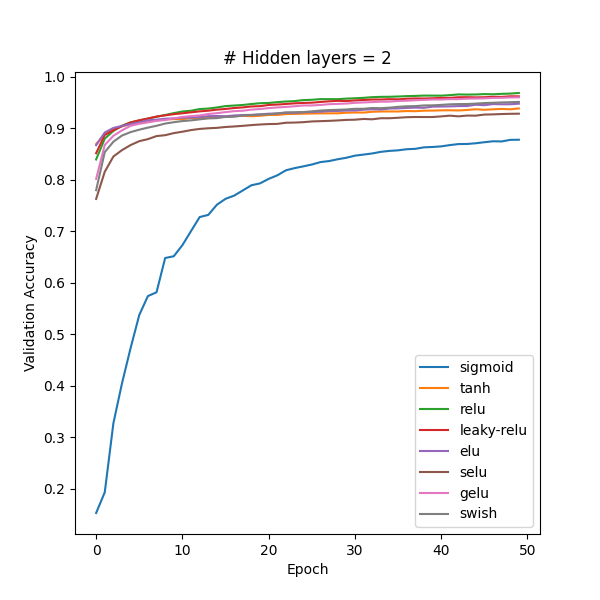
\includegraphics[width=0.4\textwidth]{images/2_hidden_layers_acc.png}
        }%
        \subfigure[Giá trị mất mát tập kiểm định (2)]{%
           \label{fig:mnistd1b}
           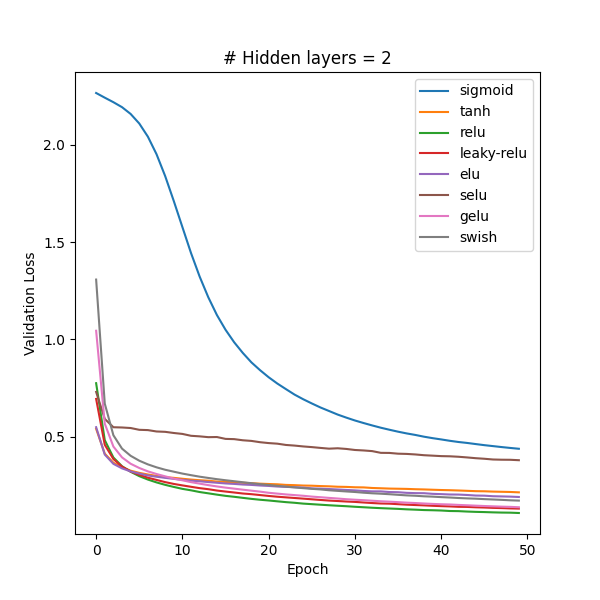
\includegraphics[width=0.4\textwidth]{images/2_hidden_layers_loss.png}
        }\\ %  ------- End of the first row ----------------------%
        \subfigure[Giá trị chính xác tập kiểm định (3)]{%
            \label{fig:mnistd1c}
            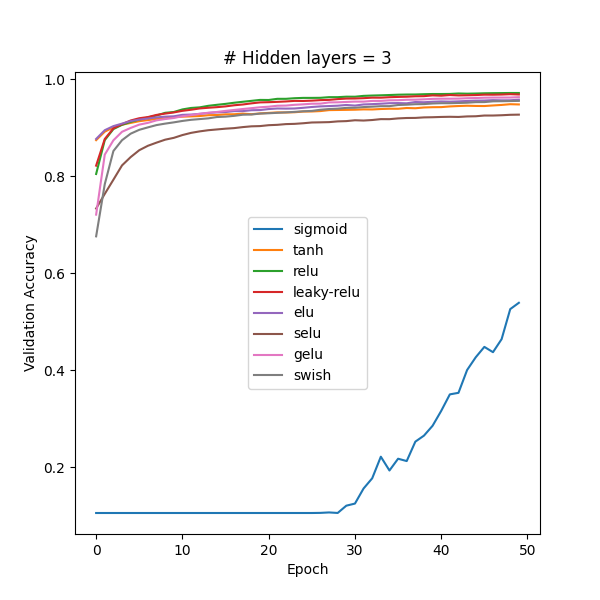
\includegraphics[width=0.4\textwidth]{images/3_hidden_layers_acc.png}
        }%
        \subfigure[Giá trị mất mát tập kiểm định (3)]{%
            \label{fig:mnistd1d}
            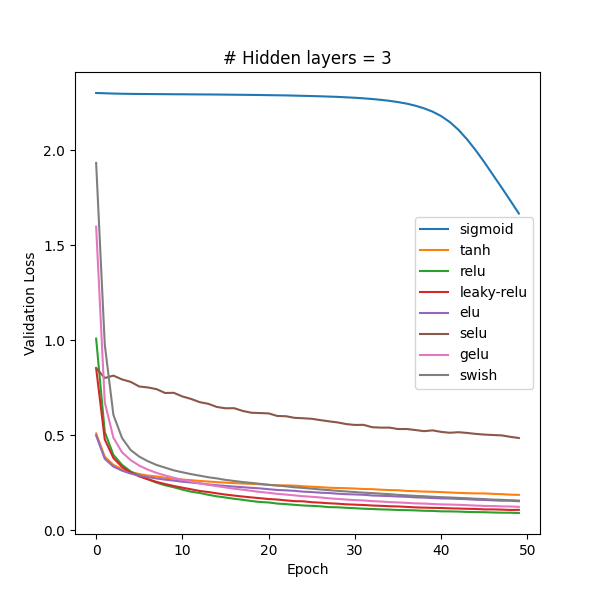
\includegraphics[width=0.4\textwidth]{images/3_hidden_layers_loss.png}
        }\\
        %----------------------%
        \subfigure[Giá trị chính xác tập kiểm định (4)]{%
            \label{fig:mnistd1e}
            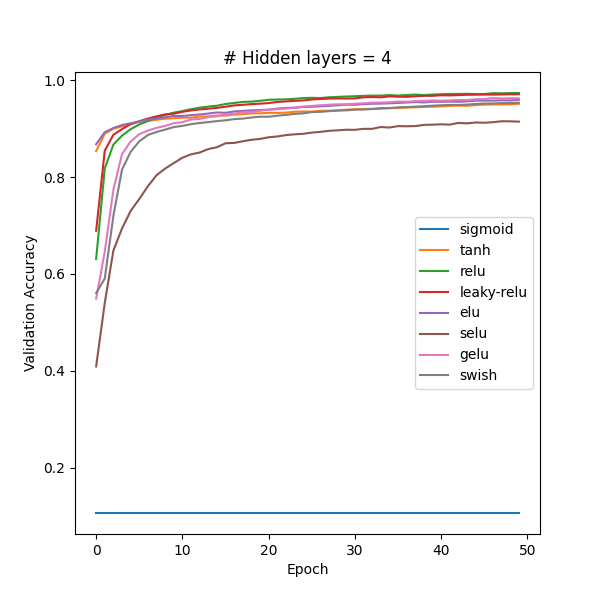
\includegraphics[width=0.4\textwidth]{images/4_hidden_layers_acc.png}
        }%
        \subfigure[Giá trị mất mát tập kiểm định (4)]{%
            \label{fig:mnistd1f}
            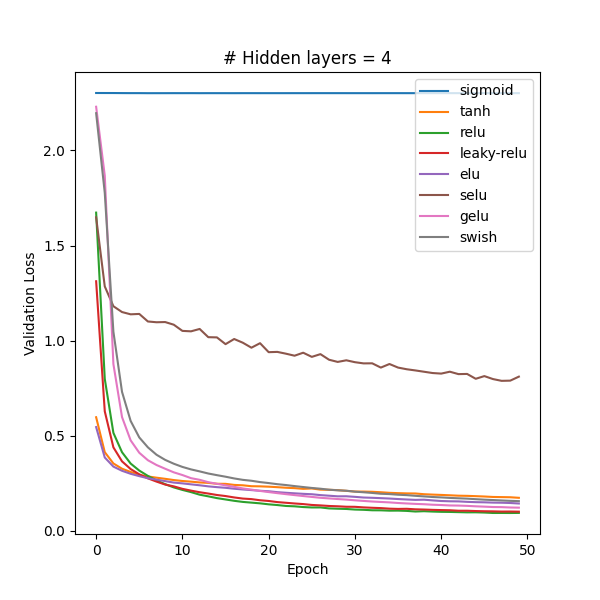
\includegraphics[width=0.4\textwidth]{images/4_hidden_layers_loss.png}
        }%
%
    \end{center}
    \caption{%
        Giá trị chính xác và mất mát (chuẩn hoá Lecun) trên tập kiểm định (số tầng ẩn: 2, 3, 4).
     }%
   \label{fig:mnistd1}
\end{figure}

\begin{figure}[ht!]
     \begin{center}
%
        \subfigure[Giá trị chính xác tập kiểm định (5)]{%
            \label{fig:mnistd2a}
            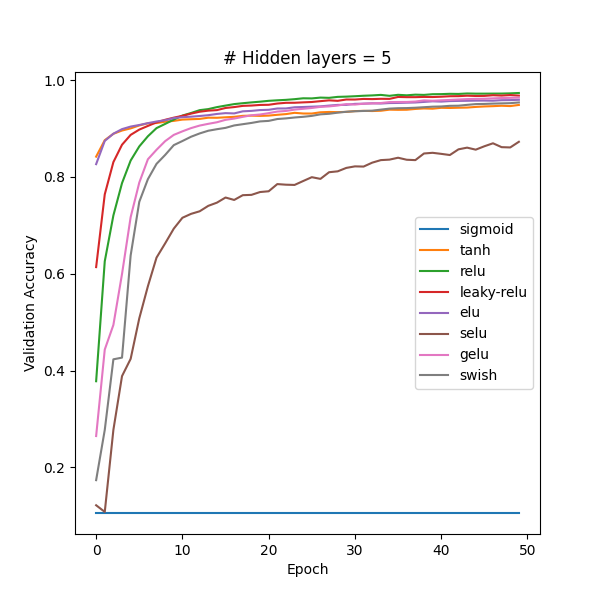
\includegraphics[width=0.4\textwidth]{images/5_hidden_layers_acc.png}
        }%
        \subfigure[Giá trị mất mát tập kiểm định (5)]{%
           \label{fig:mnistd2b}
           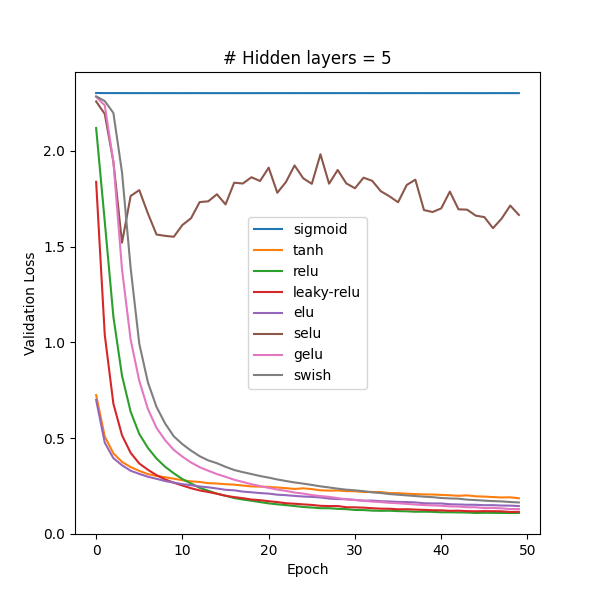
\includegraphics[width=0.4\textwidth]{images/5_hidden_layers_loss.png}
        }\\ %  ------- End of the first row ----------------------%
        \subfigure[Giá trị chính xác tập kiểm định (6)]{%
            \label{fig:mnistd2c}
            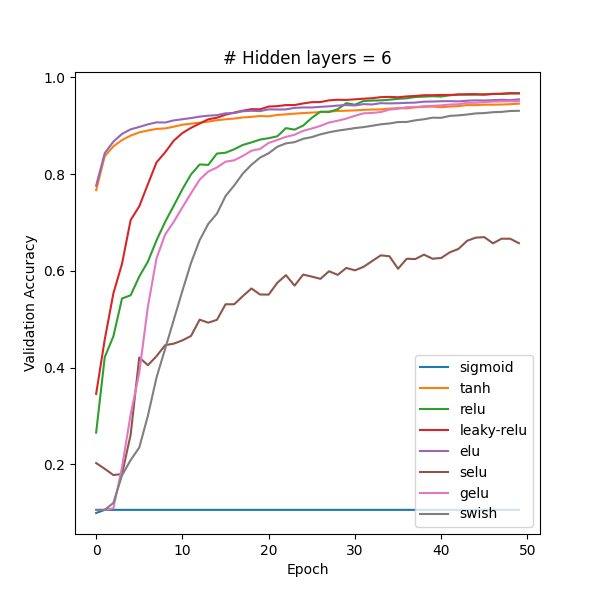
\includegraphics[width=0.4\textwidth]{images/6_hidden_layers_acc.png}
        }%
        \subfigure[Giá trị mất mát tập kiểm định (6)]{%
            \label{fig:mnistd2d}
            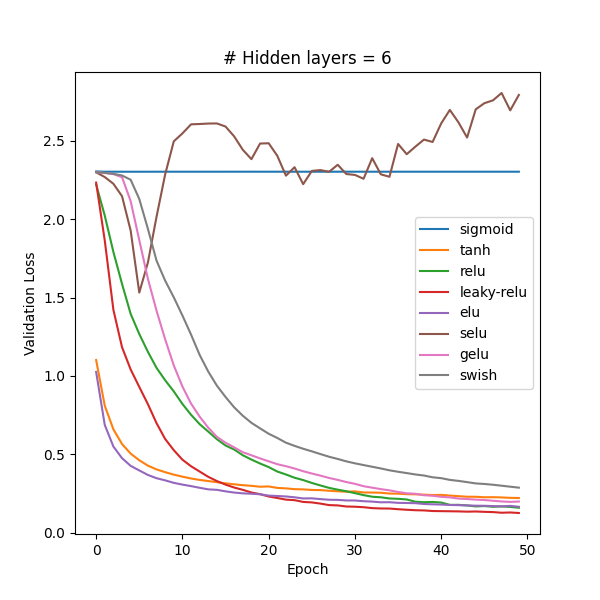
\includegraphics[width=0.4\textwidth]{images/6_hidden_layers_loss.png}
        }\\
        %----------------------%
        \subfigure[Giá trị chính xác tập kiểm định (7)]{%
            \label{fig:mnistd2e}
            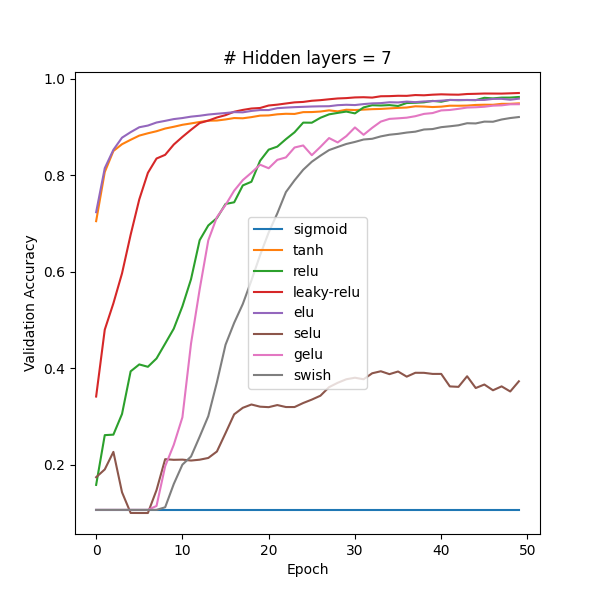
\includegraphics[width=0.4\textwidth]{images/7_hidden_layers_acc.png}
        }%
        \subfigure[Giá trị mất mát tập kiểm định (7)]{%
            \label{fig:mnistd2f}
            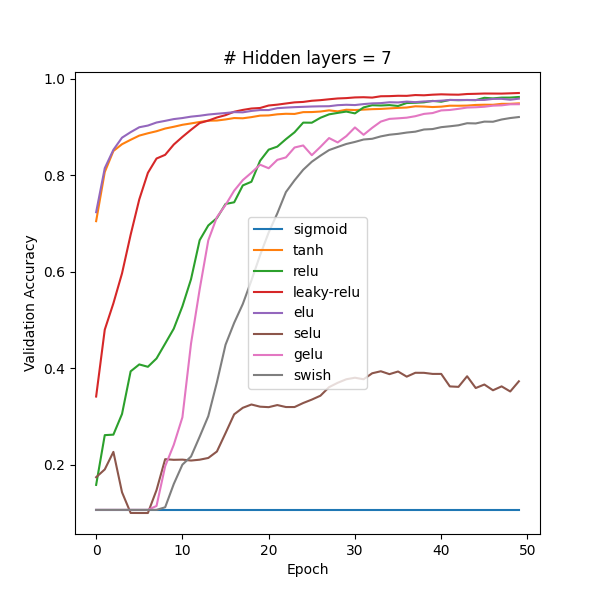
\includegraphics[width=0.4\textwidth]{images/7_hidden_layers_acc.png}
        }%
%
    \end{center}
    \caption{%
        Giá trị chính xác và mất mát (chuẩn hoá Lecun) trên tập kiểm định (số tầng ẩn: 5, 6, 7).
     }%
   \label{fig:mnistd2}
\end{figure}

\begin{figure}[ht!]
     \begin{center}
%
        \subfigure[Giá trị chính xác tập kiểm định (8)]{%
            \label{fig:mnistd3a}
            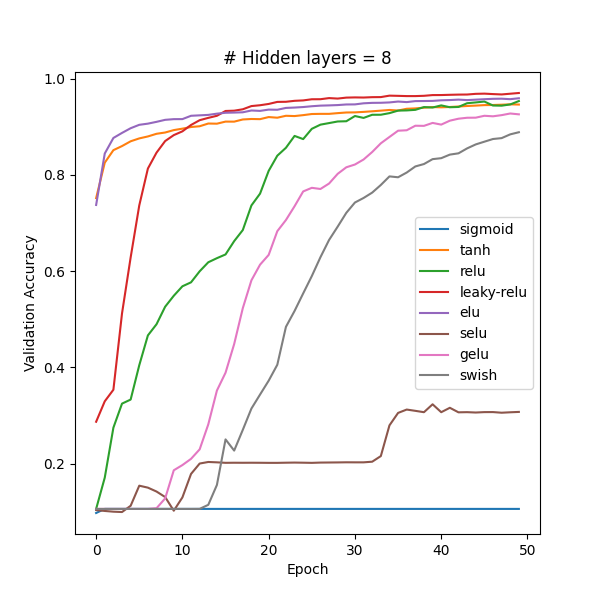
\includegraphics[width=0.4\textwidth]{images/8_hidden_layers_acc.png}
        }%
        \subfigure[Giá trị mất mát tập kiểm định (8)]{%
           \label{fig:mnistd3b}
           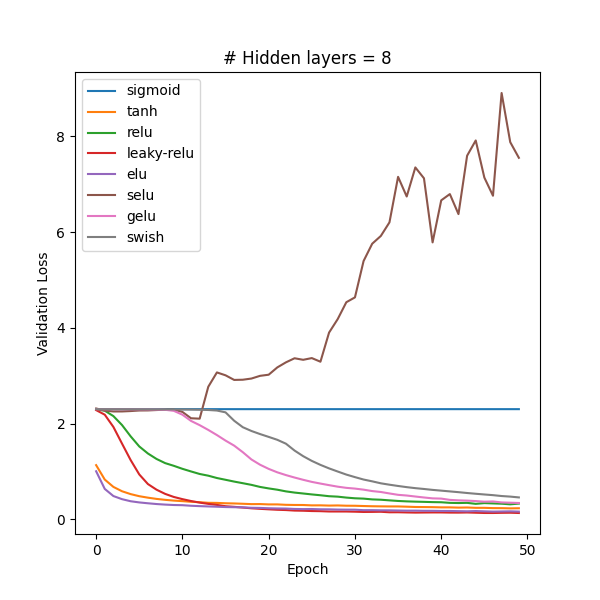
\includegraphics[width=0.4\textwidth]{images/8_hidden_layers_loss.png}
        }\\ %  ------- End of the first row ----------------------%
        \subfigure[Giá trị chính xác tập kiểm định (9)]{%
            \label{fig:mnistd3c}
            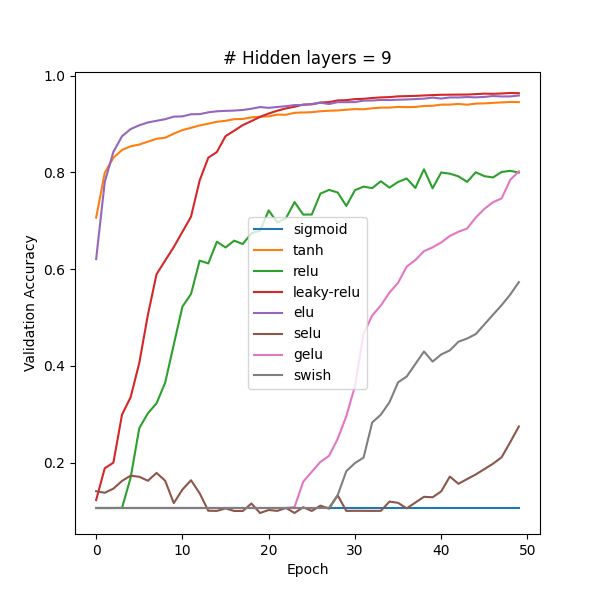
\includegraphics[width=0.4\textwidth]{images/9_hidden_layers_acc.png}
        }%
        \subfigure[Giá trị mất mát tập kiểm định (9)]{%
            \label{fig:mnistd3d}
            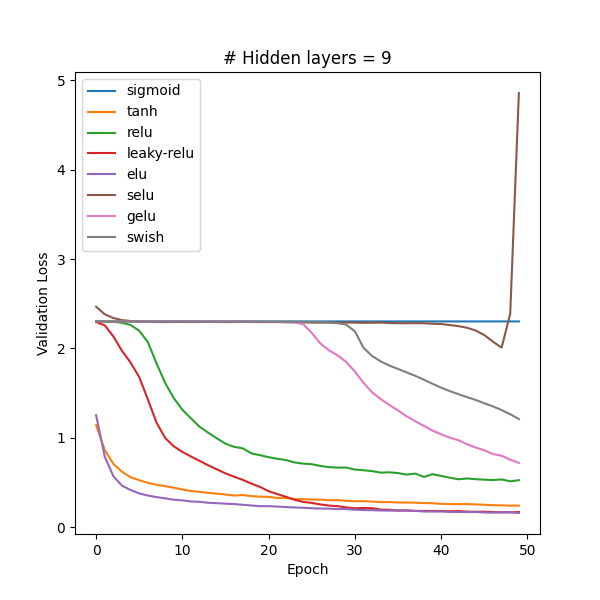
\includegraphics[width=0.4\textwidth]{images/9_hidden_layers_loss.png}
        }\\
        %----------------------%
        \subfigure[Giá trị chính xác tập kiểm định (10)]{%
            \label{fig:mnistd3e}
            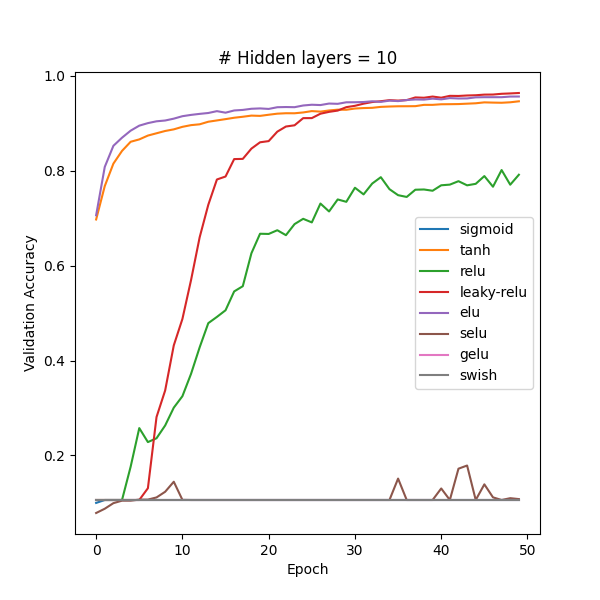
\includegraphics[width=0.4\textwidth]{images/10_hidden_layers_acc.png}
        }%
        \subfigure[Giá trị mất mát tập kiểm định (10)]{%
            \label{fig:mnistd3f}
            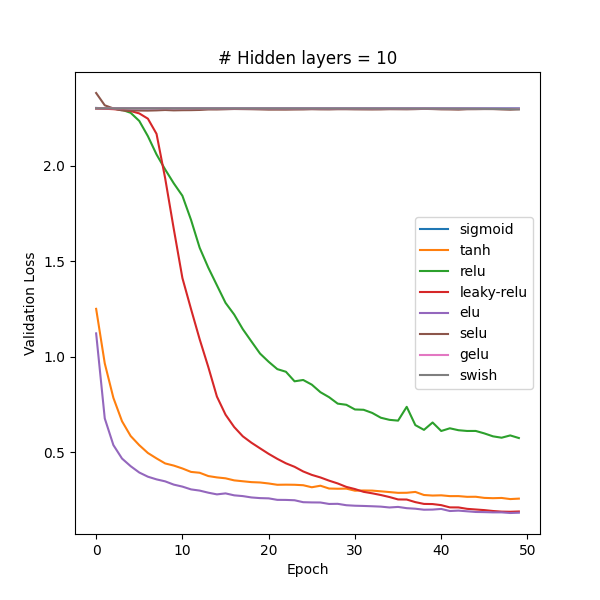
\includegraphics[width=0.4\textwidth]{images/10_hidden_layers_loss.png}
        }%
%
    \end{center}
    \caption{%
        Giá trị chính xác và mất mát (chuẩn hoá Lecun) trên tập kiểm định (số tầng ẩn: 8, 9, 10).
     }%
   \label{fig:mnistd3}
\end{figure}

\begin{figure}[ht!]
     \begin{center}
%
        \subfigure[Giá trị chính xác tập kiểm định (11)]{%
            \label{fig:mnistd4a}
            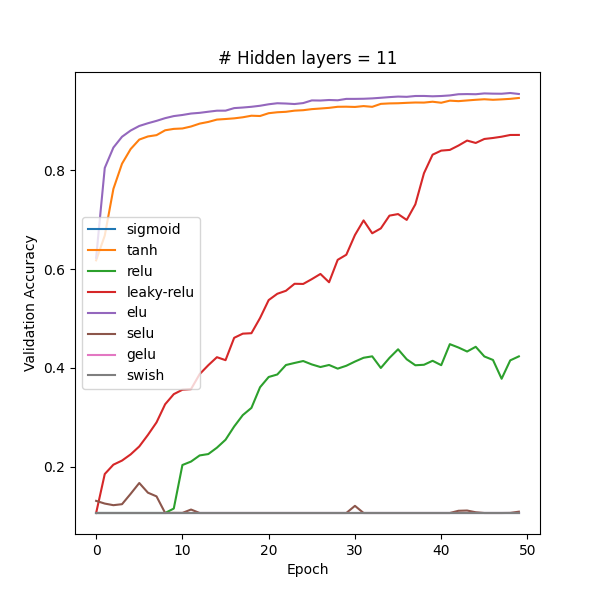
\includegraphics[width=0.4\textwidth]{images/11_hidden_layers_acc.png}
        }%
        \subfigure[Giá trị mất mát tập kiểm định (11)]{%
           \label{fig:mnistd4b}
           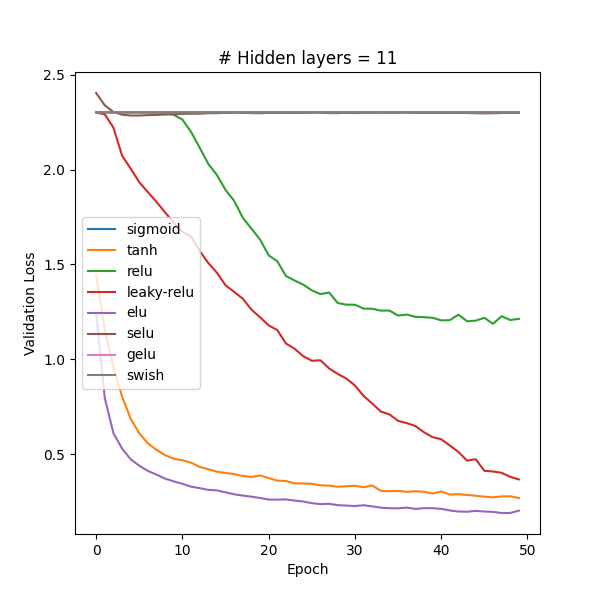
\includegraphics[width=0.4\textwidth]{images/11_hidden_layers_loss.png}
        }\\ %  ------- End of the first row ----------------------%
        \subfigure[Giá trị chính xác tập kiểm định (12)]{%
            \label{fig:mnistd4c}
            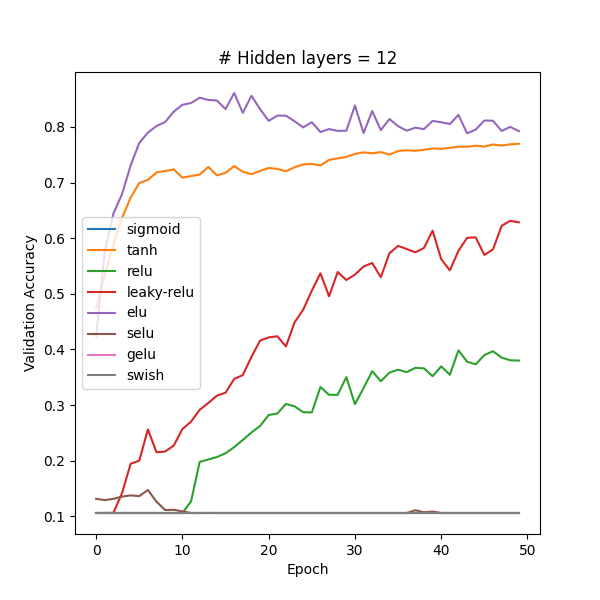
\includegraphics[width=0.4\textwidth]{images/12_hidden_layers_acc.png}
        }%
        \subfigure[Giá trị mất mát tập kiểm định (12)]{%
            \label{fig:mnistd4d}
            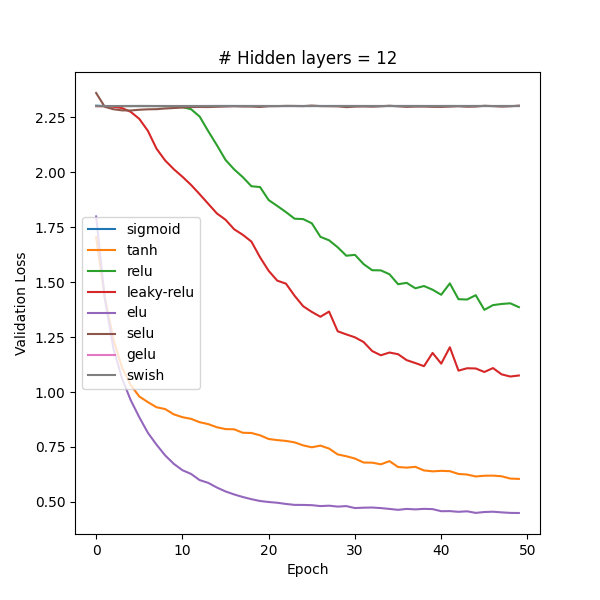
\includegraphics[width=0.4\textwidth]{images/12_hidden_layers_loss.png}
        }\\
        \subfigure[Giá trị chính xác so với số tầng ẩn]{%
            \label{fig:mnistd4e}
            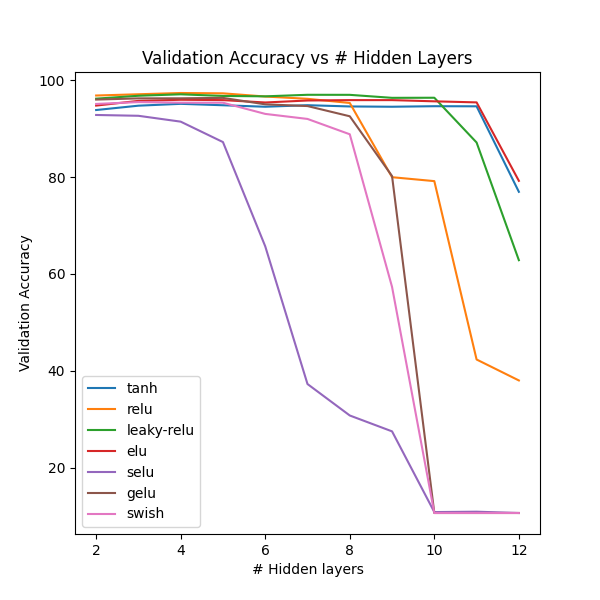
\includegraphics[width=0.4\textwidth]{images/vs_acc_hiddenlayers.png}
        }%
        \subfigure[Giá trị mất mát so với số tầng ẩn]{%
           \label{fig:mnistd4f}
           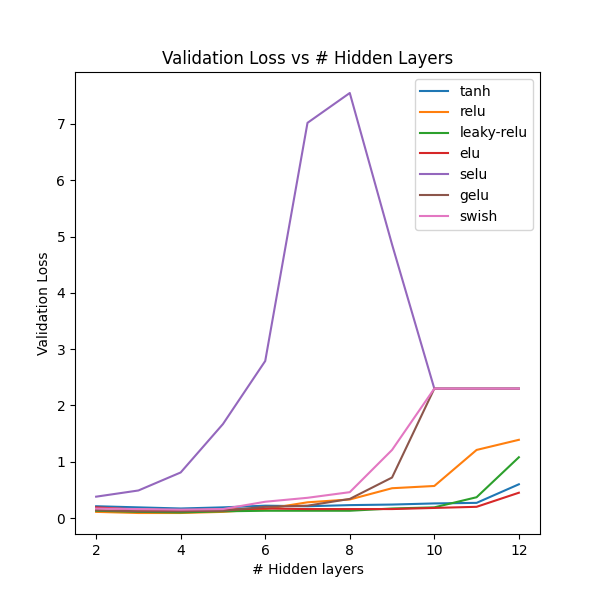
\includegraphics[width=0.4\textwidth]{images/vs_loss_hiddenlayers.png}
        }
%
    \end{center}
    \caption{%
        Giá trị chính xác và mất mát (chuẩn hoá Lecun) trên tập kiểm định (số tầng ẩn: 11, 12) [(a) - (d)]; Giá trị chính xác và mất mát (chuẩn hoá Lecun) trên tập kiểm định so với số tầng ẩn [(e), (f)].
     }%
   \label{fig:mnistd4}
\end{figure}

\clearpage

\subsection{Dữ liệu có nhiễu Gauss và khởi tạo trọng số theo chuẩn hoá Lecun}\label{subsec:mnistnoise}

Dữ liệu bây giờ được tạo nhiễu theo hàm Gauss có độ lệch chuẩn $\sigma = 0.2$.
Hình \ref{fig:mnistexamplerawandnoise} cho ta thấy sự khác biệt giữa mẫu nguyên thuỷ và mẫu khi có nhiễu tác động vào.
Khoảng giá trị bây giờ của các phần tử trong mẫu nhiễu có thể âm (tức < 0) và cũng có thể lơn hơn 1.
Như trong ảnh \ref{fig:mnist5noise} có phần tử điểm ảnh có giá trị nhỏ nhất và lớn nhất lần lượt là $-0.5876574$ và $1.4352913$.

\begin{figure}[ht!]
     \begin{center}
%
        \subfigure[Ảnh chữ số 5 trong tập dữ liệu MNIST]{%
            \label{fig:mnist5raw}
            
\includegraphics[width=0.4\textwidth]{images/mnistraw.png}
        }%
        \subfigure[Ảnh chữ số 5 khi thêm nhiễu Gauss $\left(\sigma = 0.2\right)$ trong tập dữ liệu MNIST]{%
          \label{fig:mnist5noise}
          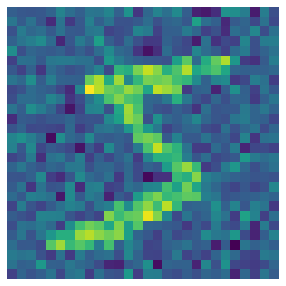
\includegraphics[width=0.4\textwidth]{images/mnistnoise.png}
        }
%
    \end{center}
    \caption{%
        Ví dụ về ảnh trước và sau khi thêm nhiễu Gauss từ tập dữ liệu MNIST.
     }%
  \label{fig:mnistexamplerawandnoise}
\end{figure}

Cách thức huấn luyện vẫn được áp dụng như phần \ref{subsec:mnistd}, tuy nhiên lần này có một chút khác biệt là kỹ thuật alpha dropout sẽ không được áp dụng cho SELU mà sẽ sử dụng cách dropout bình thường với cùng tỷ lệ như các hàm kích hoạt khác.
Biểu đồ giá trị chính xác và mất mát trên tập kiểm định qua mỗi epoch được cho ở các hình \ref{fig:mnistnoise1}, \ref{fig:mnistnoise2}, \ref{fig:mnistnoise3}, \ref{fig:mnistnoise4}.
Chi tiết về giá trị được cho ở bảng \ref{tab:mnistnoiseacc} và bảng \ref{tab:mnistnoiseloss}.

\begin{table}[ht!]
\centering
\def\arraystretch{1.1}
\begin{tabular}{c|c|c|c|c|c|c|c|c|c|c|c|}
\cline{2-12}
                        & 2     & 3     & 4     & 5     & 6     & 7     & 8     & 9     & 10    & 11    & 12    \\ \hline
\multicolumn{1}{|c|}{$\tanh$} & 92.14 & 93.10 & 93.40 & 93.09 & 92.83 & 93.35 & 92.98 & 92.74 & 92.86 & 92.13 & 67.80 \\ \hline
\multicolumn{1}{|c|}{$\mathcal{R}$} & \textbf{95.46} & \textbf{95.88} & \textbf{95.97} & \textbf{95.78} & 94.57 & 93.83 & 91.21 & 86.59 & 42.95 & 40.26 & 45.08 \\ \hline
\multicolumn{1}{|c|}{$\mathcal{R}_L$} & 94.83 & 95.18 & 95.55 & 95.14 & \textbf{94.63} & \textbf{95.04} & \textbf{95.10} & \textbf{94.01} & 93.08 & 73.42 & 54.34 \\ \hline
\multicolumn{1}{|c|}{$\mathcal{E}$} & 93.03 & 94.23 & 94.52 & 94.43 & 93.86 & 94.30 & 94.13 & 93.99 & 93.98 & \textbf{93.94} & \textbf{84.06} \\ \hline
\multicolumn{1}{|c|}{$\mathcal{E}_S$} & 91.46 & 93.10 & 93.76 & 93.66 & 93.32 & 94.12 & 94.31 & 93.06 & \textbf{94.03} & 93.77 & 68.40 \\ \hline
\multicolumn{1}{|c|}{$\mathcal{G}$} & 95.02 & 95.38 & 95.48 & 95.17 & 93.31 & 93.55 & 87.75 & 70.12 & 10.60 & 10.60 & 10.60 \\ \hline
\multicolumn{1}{|c|}{$\mathcal{S}$} & 94.08 & 94.42 & 94.42 & 94.02 & 92.34 & 88.00 & 80.94 & 46.26 & 21.84 & 10.60 & 10.60 \\ \hline
\end{tabular}
\caption{Giá trị chính xác (\%) của các hàm kích hoạt (nhiễu Gauss + chuẩn hoá Lecun) tương ứng với các số tầng ẩn của mô hình trên tập dữ liệu MNIST.}
\label{tab:mnistnoiseacc}
\end{table}

\begin{table}[ht!]
\centering
\def\arraystretch{1.3}
\begin{tabular}{c|c|c|c|c|c|c|c|c|c|c|c|}
\cline{2-12}
                        & 2    & 3    & 4    & 5    & 6    & 7    & 8    & 9    & 10   & 11   & 12   \\ \hline
\multicolumn{1}{|c|}{$\tanh$} & 0.26 & 0.23 & 0.22 & 0.25 & 0.28 & 0.28 & 0.30 & 0.31 & 0.34 & 0.37 & 0.77 \\ \hline
\multicolumn{1}{|c|}{$\mathcal{R}$} & \textbf{0.15} & \textbf{0.13} & \textbf{0.15} & \textbf{0.17} & 0.31 & 0.36 & 0.49 & 0.59 & 1.35 & 1.30 & 1.48 \\ \hline
\multicolumn{1}{|c|}{$\mathcal{R}_L$} & 0.17 & 0.15 & 0.16 & \textbf{0.17} & \textbf{0.23} & \textbf{0.21} & \textbf{0.22} & 0.34 & 0.38 & 0.78 & 1.24 \\ \hline
\multicolumn{1}{|c|}{$\mathcal{E}$} & 0.23 & 0.19 & 0.18 & 0.19 & \textbf{0.23} & \textbf{0.21} & \textbf{0.22} & \textbf{0.24} & \textbf{0.25} & \textbf{0.27} & \textbf{0.51} \\ \hline
\multicolumn{1}{|c|}{$\mathcal{E}_S$} & 0.29 & 0.24 & 0.21 & 0.21 & 0.24 & 0.23 & 0.23 & 0.25 & 0.26 & 0.28 & 0.72 \\ \hline
\multicolumn{1}{|c|}{$\mathcal{G}$} & 0.16 & 0.15 & \textbf{0.15} & \textbf{0.17} & 0.29 & 0.28 & 0.57 & 0.94 & 2.30 & 2.30 & 2.30 \\ \hline
\multicolumn{1}{|c|}{$\mathcal{S}$} & 0.20 & 0.18 & 0.19 & 0.21 & 0.30 & 0.48 & 0.65 & 1.50 & 2.02 & 2.30 & 2.30 \\ \hline
\end{tabular}
\caption{Giá trị mất mát của các hàm kích hoạt (nhiễu Gauss + chuẩn hoá Lecun) tương ứng với các mô hình trên tập dữ liệu MNIST.}
\label{tab:mnistnoiseloss}
\end{table}

Ở những kiến trúc đầu tiên, chẳng hạn khi độ sâu tầng ẩn là 2 (hình \ref{fig:mnistnoise1a}, \ref{fig:mnistnoise1a}), chưa có sự phân hoá rõ ràng giữa các hàm.
Nếu tính chi ly, thì ta có 2 cái tên quen thuộc ở những lượt đầu là RELU và Leaky có độ chính xác cao nhất (95.46\% và 94.83\%).
Trong nhóm có độ chính xác $\approx$ 95\% thì có GELU (95.02\%) - hàm không cho kết quả không khả quan ở phần thực nghiệm trước (phần \ref{subsec:mnistd}).
\vspace{5pt}

Khi số tầng ẩn đã là 5 (hình \ref{fig:mnistnoise2a}, \ref{fig:mnistnoise2a}), chất lượng độ chính xác của các hàm kích hoạt vẫn chưa phân nhóm khi tất cả đều xấp xỉ khoảng 94-95\%.
Hàm Tanh có tốc độ hội tụ khá nhanh khi chỉ cần 15 epoch để đạt ngưỡng (bảng \ref{tab:mnistnoiseepoch}).
Dẫu vậy, rõ ràng là nhận định hàm Tanh tìm được hố cực tiểu nông là một nhận định hợp lý khi sau 50 epoch, giá trị mất mát của hàm này không thay đổi nhiều và đứng ở 0.25, trở thành hàm có mất mát cao nhất trong lượt này.

\begin{table}[ht!]
\centering
\def\arraystretch{1.3}
\begin{tabular}{c|c|c|c|c|c|c|c|c|c|c|c|c|}
\cline{2-13}
                        & 2  & 3  & 4  & 5  & 6  & 7  & 8  & 9  & 10 & 11 & 12 & $\mu$ \\ \hline
\multicolumn{1}{|c|}{$\tanh$} & 10 & 20 & \textbf{20} & \textbf{15} & 19 & \textbf{23} & \textbf{16} & \textbf{22} & 24 & 31 & 15 & \textbf{20}\\ \hline
\multicolumn{1}{|c|}{$\mathcal{R}$} & 29 & 31 & 24 & 27 & 29 & 36 & 33 & 41 & \textbf{18} & 26 & 16 & 28\\ \hline
\multicolumn{1}{|c|}{$\mathcal{R}_L$} & 29 & 30 & 26 & 27 & 28 & 26 & 28 & 29 & 40 & 35 & 30 & 30\\ \hline
\multicolumn{1}{|c|}{$\mathcal{E}$} & 20 & 29 & 29 & 27 & 25 & 25 & 25 & 25 & 28 & \textbf{23} & 30 & 26\\ \hline
\multicolumn{1}{|c|}{$\mathcal{E}_S$} & \textbf{4}  & \textbf{16} & 22 & 22 & \textbf{18} & \textbf{23} & 22 & \textbf{22} & 24 & 26 & \textbf{9}  & \textbf{20}\\ \hline
\multicolumn{1}{|c|}{$\mathcal{G}$} & 34 & 33 & 33 & 32 & 38 & 40 & 46 & 46 & 1  & 1  & 1  & X\\ \hline
\multicolumn{1}{|c|}{$\mathcal{S}$} & 31 & 33 & 31 & 33 & 39 & 39 & 44 & 41 & 1  & 1  & 1  & X\\ \hline
\end{tabular}
\caption{Số epoch cần thiết để 80\% giá trị mất mát (nhiễu Gauss + chuẩn hoá Lecun) bằng giá trị mất mát cuối cùng.}
\label{tab:mnistnoiseepoch}
\end{table}

Tới 7 tầng ẩn (hình \ref{fig:mnistnoise2e}, \ref{fig:mnistnoise2f}), Swish là cái tên đầu tiên có vẽ không còn đủ khả năng để đi tiếp.
Tuy RELU và GELU có màn thể hiện rất tốt ở gian đoạn đầu, nhưng cũng như lần thử nghiệm trước (phần \ref{subsec:mnistd}), khi số tầng ẩn khá sâu thì đã giảm hiệu quả của 2 hàm này.
Leaky tuy hội tụ khá chậm so với nhóm đầu - nhóm gồm Tanh, ELU và SELU khi phải mất tới 36 epoch mới đạt ngưỡng, nhưng về cuối lại có một kết quả chính xác tốt khi vẫn trên 90\% và cao hơn cả hàm Tanh (93.83\% > 92.92\%).
Một điểm khá bất ngờ là khi không áp dụng alpha dropout, SELU đạt kết quả rất tốt.
Không chỉ có giá trị chính xác cao, mất mát thấp mà việc hội tụ cũng rất nhanh khi đạt ngưỡng sau 23 epoch, ngang với hàm dễ đạt ngưỡng như Tanh.
\vspace{5pt}

Hình \ref{fig:mnistnoise3c} và hình \ref{fig:mnistnoise3d} cho thấy rằng GELU không còn có thể duy trì được phong độ như RELU đang làm.
Tuy là RELU có vẻ không phù hợp cho những mạng sâu, nhưng giá trị chính xác và mất mát không ở mức quá tệ (chính xác 86.59\% và mất mát 0.59).
Leaky giờ đây đã tụt xuống ngang với hàm Tanh, dẫn đến việc ta thấy Leaky hội tụ rất lâu, và phải tới 41 epoch mới đạt ngưỡng.
ELU và người anh em SELU của mình nổi trội với độ chính xác 94\% $\pm$ 0.01\%.
Ngoài ra 2 hàm trên, còn Tanh và Leaky là hai hàm có giá trị chính xác trên tập kiểm định trên 90\% sau 50 epoch.
Điều này được kéo dài và kết thúc ngay khi số tầng ẩn tăng lên 11 (hình \ref{fig:mnistnoise4a}, \ref{fig:mnistnoise4b}) khi giá trị chính xác Leaky lúc này chỉ còn 73.42\%, trong khi 3 hàm Tanh, ELU và SELU vẫn trên 90\%.
\vspace{5pt}

Ở kiến trúc cuối cùng - 12 tầng ẩn (hình \ref{fig:mnistnoise4c}, \ref{fig:mnistnoise4d}), có 3 nhóm tách biệt khá rõ rệt (không tính những hàm không còn khả năng học là GELU và Swish).
Nhóm kết quả thấp nhất là RELU và Leaky với độ chính xác tầm khoảng 50\% (45.05\% và 54.34\%) và mất mát cao hơn 1.0 (1.48 và 1.24).
Nhóm giữa là Tanh và SELU với mất mát xấp xỉ nhau với mất mát là 0.77 và 0.72, giá trị chính xác của cả hai $\approx$ 68\%.
Nhóm có kết quả tốt nhất và cũng chỉ duy nhất ELU khi giá trị chính xác là 84.06\% (vẫn trên 80\%).

\begin{table}[ht!]
\centering
\def\arraystretch{1.5}
\begin{tabular}{c|c|c|c|c|c|c|c|}
\cline{2-8}
                        & $\tanh$      & $\mathcal{R}$      & $\mathcal{R}_L$      & $\mathcal{E}$      & $\mathcal{E}_S$      & $\mathcal{G}$      & $\mathcal{S}$      \\ \hline
\multicolumn{1}{|c|}{$\mu_{\text{chính xác}}$ (\%)} & 90.58  & 79.78  & 89.12  & \textbf{93.13}  & 91.27  & 68.87  & 66.14  \\ \hline
\multicolumn{1}{|c|}{$\sigma^2_{\text{chính xác}} (\%)$} & 0.0052 & 0.0522 & 0.0159 & \textbf{0.0008} & 0.0053 & 0.1321 & 0.1188 \\ \hline
\multicolumn{1}{|c|}{$\mu_{\text{mất mát}}$} & 0.33   & 0.59   & 0.37   & \textbf{0.25}   & 0.29   & 0.88   & 0.94   \\ \hline
\multicolumn{1}{|c|}{$\sigma^2_{\text{mất mát}}$} & 0.0215 & 0.2526 & 0.1068 & \textbf{0.0072} & 0.0194 & 0.8121 & 0.7380 \\ \hline
\end{tabular}
\caption{Giá trị trung bình và phương sai của các hàm kích hoạt (nhiễu Gauss + chuẩn hoá Lecun) trong 11 mô hình thử nghiệm.}
\label{tab:mnistnoisemean}
\end{table}

Kết quả của lần thực nghiệm này không có quá nhiều khác biệt (hình \ref{fig:mnistnoise4e}, \ref{fig:mnistnoise4f}) so với lần thử nghiệm khi tập dữ liệu không có nhiễu (phần \ref{subsec:mnistd}).
Hàm RELU và Leaky vẫn là những hàm nổi trội với giá trị chính xác cao trong những mô hình có độ sâu vừa phải.
Về hàm Tanh, vẫn là một hàm không thể hiện được sức mạnh ở những mô hình đầu như RELU hay Leaky khi nhanh chóng tìm một hố sâu cực tiểu.
Tuy vậy, điều này lại vẫn là lợi thế khi tầng ẩn trong các mạng được nâng lên, đó là lí do mà Tanh có $\mu_{\text{chính xác}} = 90.58\%$ sau 11 mô hình.
ELU vẫn là hàm có kết quả tốt nhất với $\mu_{\text{chính xác}} = 93.13\%$ và $\mu_{\text{mất mát}} = 0.25$.
SELU cũng có kết quả rất khả quan sau khi loại bỏ đi kỷ thuật alpha dropout cho mô hình có hàm kích hoạt này khi có $\mu_{\text{chính xác}} = 91.27\%$ (chỉ thua mỗi ELU).
Một ấn tượng nữa của SELU là nó cũng có tốc độ hội tụ khá nhanh, ngang tới Tanh.
Dẫu thế, vẫn chưa khẳng định là SELU cũng chỉ tìm hố cực tiểu nông như Tanh vì ngoại trừ 12 tầng ẩn, những mô hình còn lại SELU có giá trị mất mát cách một hàm cho kết quả tốt như ELU không quá 0.03.

\begin{figure}[ht!]
     \begin{center}
%
        \subfigure[Giá trị chính xác tập kiểm định (2)]{%
            \label{fig:mnistnoise1a}
            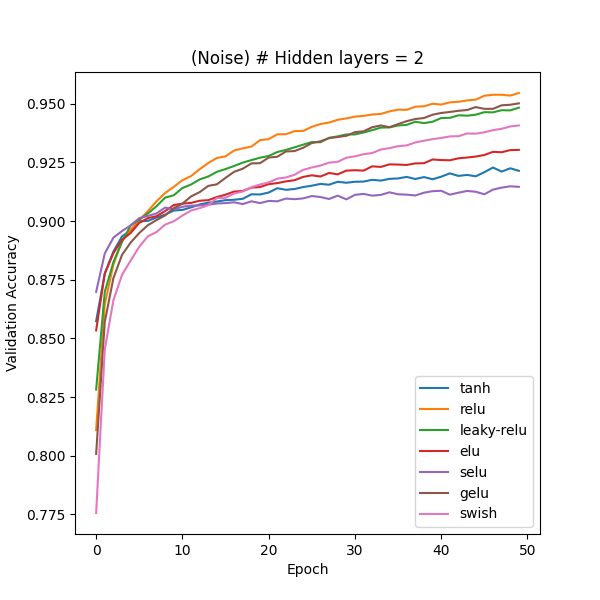
\includegraphics[width=0.4\textwidth]{images/noise_2_hidden_layers_acc.png}
        }%
        \subfigure[Giá trị mất mát tập kiểm định (2)]{%
          \label{fig:mnistnoise1b}
          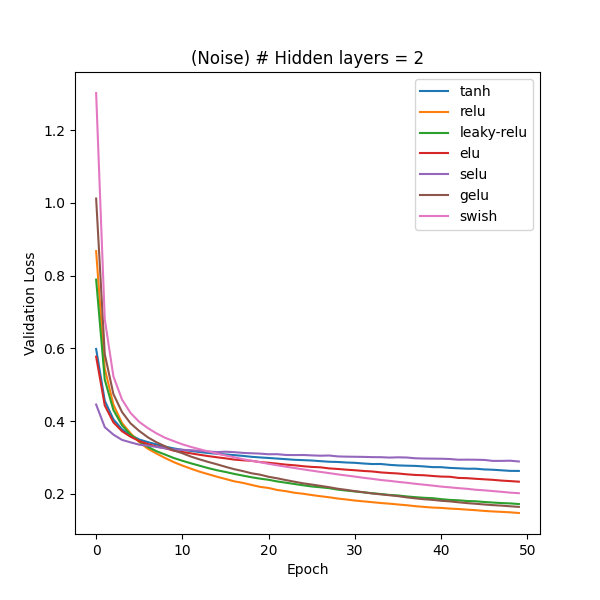
\includegraphics[width=0.4\textwidth]{images/noise_2_hidden_layers_loss.png}
        }\\ %  ------- End of the first row ----------------------%
        \subfigure[Giá trị chính xác tập kiểm định (3)]{%
            \label{fig:mnistnoise1c}
            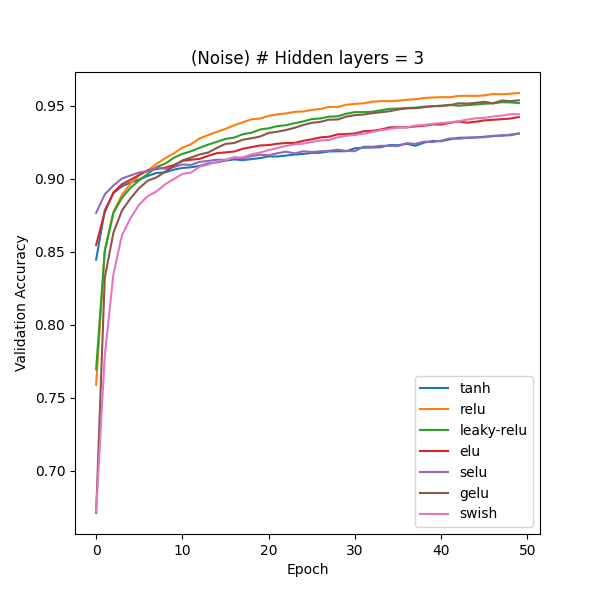
\includegraphics[width=0.4\textwidth]{images/noise_3_hidden_layers_acc.png}
        }%
        \subfigure[Giá trị mất mát tập kiểm định (3)]{%
            \label{fig:mnistnoise1d}
            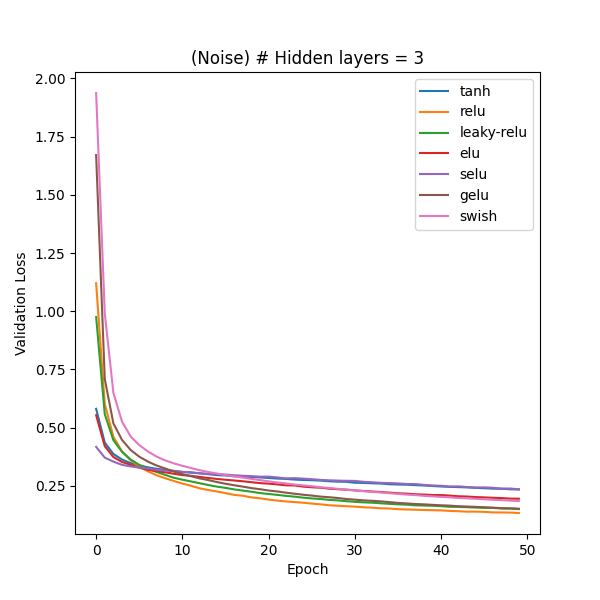
\includegraphics[width=0.4\textwidth]{images/noise_3_hidden_layers_loss.png}
        }\\
        %----------------------%
        \subfigure[Giá trị chính xác tập kiểm định (4)]{%
            \label{fig:mnistnoise1e}
            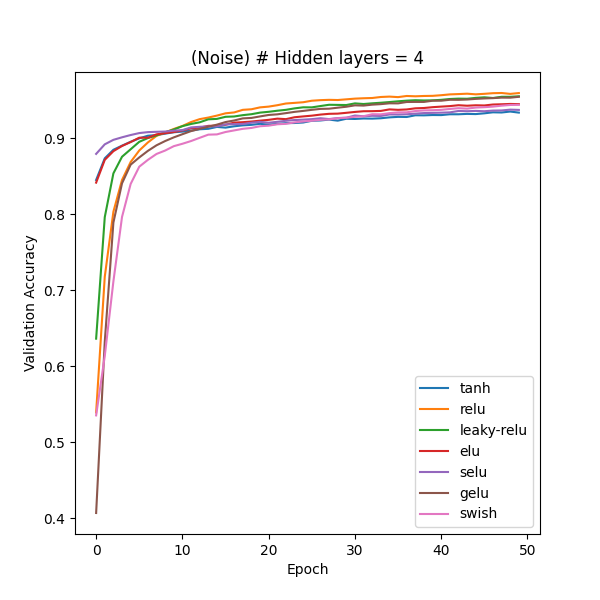
\includegraphics[width=0.4\textwidth]{images/noise_4_hidden_layers_acc.png}
        }%
        \subfigure[Giá trị mất mát tập kiểm định (4)]{%
            \label{fig:mnistnoise1f}
            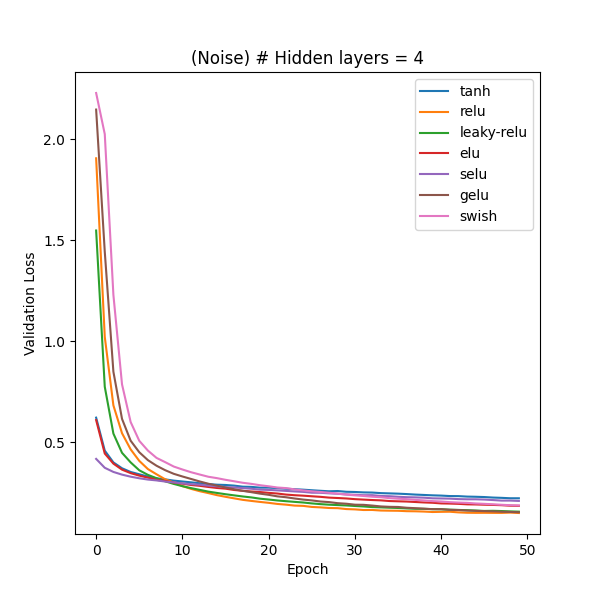
\includegraphics[width=0.4\textwidth]{images/noise_4_hidden_layers_loss.png}
        }%
%
    \end{center}
    \caption{%
        Giá trị chính xác và mất mát (nhiễu Gauss + chuẩn hoá Lecun) trên tập kiểm định (số tầng ẩn: 2, 3, 4).
     }%
  \label{fig:mnistnoise1}
\end{figure}

\begin{figure}[ht!]
     \begin{center}
%
        \subfigure[Giá trị chính xác tập kiểm định (5)]{%
            \label{fig:mnistnoise2a}
            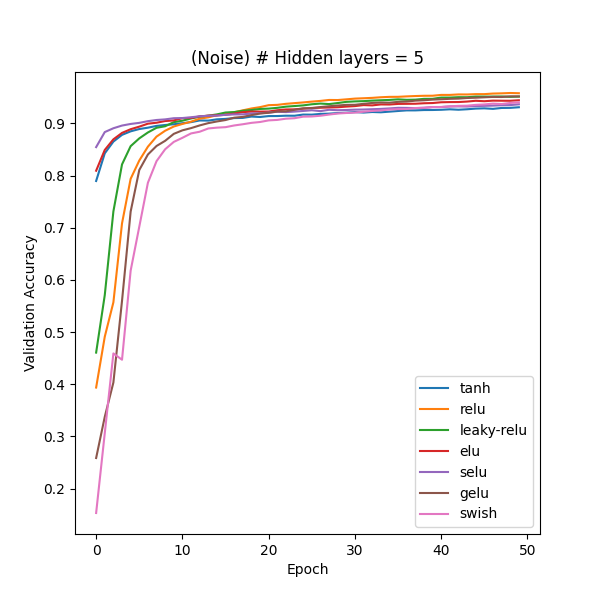
\includegraphics[width=0.4\textwidth]{images/noise_5_hidden_layers_acc.png}
        }%
        \subfigure[Giá trị mất mát tập kiểm định (5)]{%
          \label{fig:mnistnoise2b}
          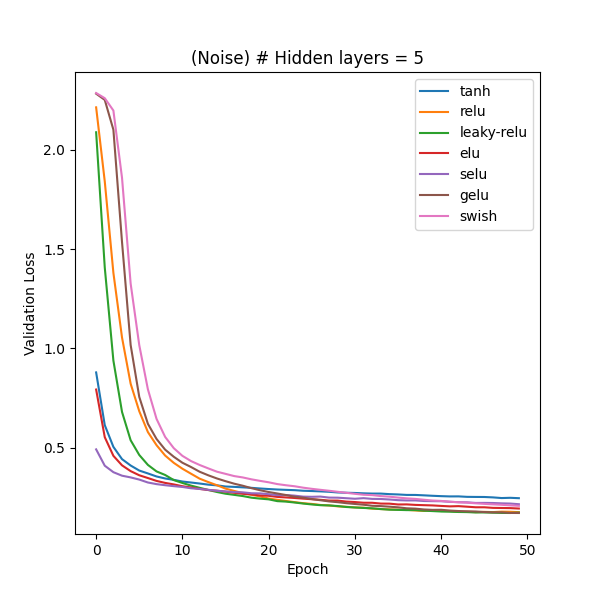
\includegraphics[width=0.4\textwidth]{images/noise_5_hidden_layers_loss.png}
        }\\ %  ------- End of the first row ----------------------%
        \subfigure[Giá trị chính xác tập kiểm định (6)]{%
            \label{fig:mnistnoise2c}
            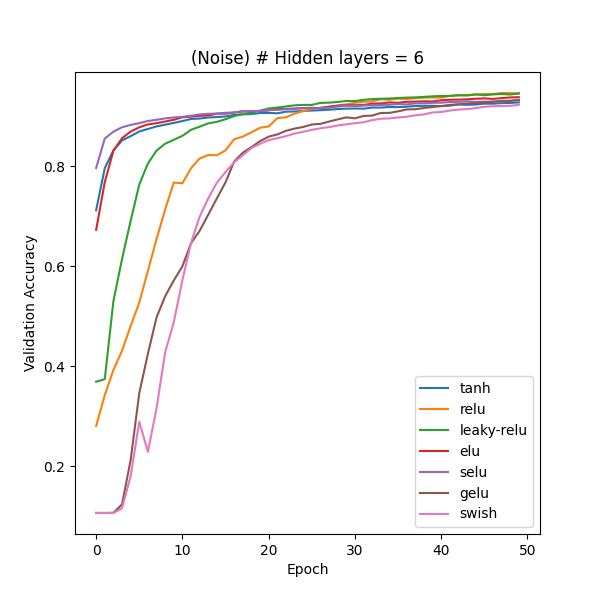
\includegraphics[width=0.4\textwidth]{images/noise_6_hidden_layers_acc.png}
        }%
        \subfigure[Giá trị mất mát tập kiểm định (6)]{%
            \label{fig:mnistnoise2d}
            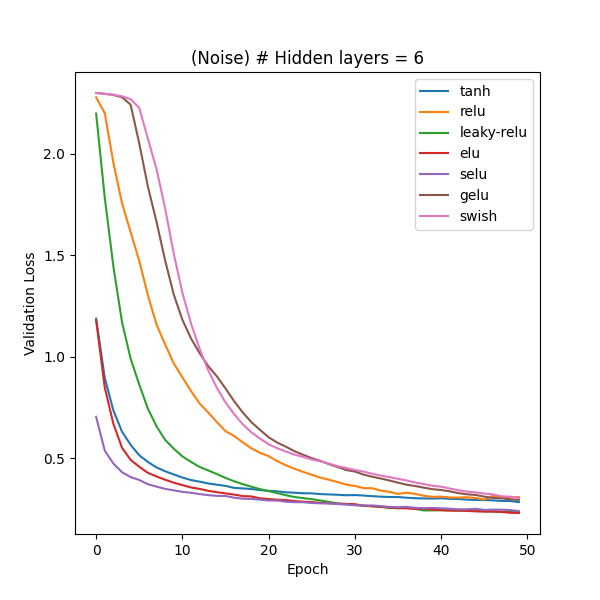
\includegraphics[width=0.4\textwidth]{images/noise_6_hidden_layers_loss.png}
        }\\
        %----------------------%
        \subfigure[Giá trị chính xác tập kiểm định (7)]{%
            \label{fig:mnistnoise2e}
            \includegraphics[width=0.4\textwidth]{images/noise_7_hidden_layers_acc.png}
        }%
        \subfigure[Giá trị mất mát tập kiểm định (7)]{%
            \label{fig:mnistnoise2f}
            \includegraphics[width=0.4\textwidth]{images/noise_7_hidden_layers_loss.png}
        }%
%
    \end{center}
    \caption{%
        Giá trị chính xác và mất mát (nhiễu Gauss + chuẩn hoá Lecun) trên tập kiểm định (số tầng ẩn: 5, 6, 7).
     }%
  \label{fig:mnistnoise2}
\end{figure}

\begin{figure}[ht!]
     \begin{center}
%
        \subfigure[Giá trị chính xác tập kiểm định (8)]{%
            \label{fig:mnistnoise3a}
            \includegraphics[width=0.4\textwidth]{images/noise_8_hidden_layers_acc.png}
        }%
        \subfigure[Giá trị mất mát tập kiểm định (8)]{%
          \label{fig:mnistnoise3b}
          \includegraphics[width=0.4\textwidth]{images/noise_8_hidden_layers_loss.png}
        }\\ %  ------- End of the first row ----------------------%
        \subfigure[Giá trị chính xác tập kiểm định (9)]{%
            \label{fig:mnistnoise3c}
            \includegraphics[width=0.4\textwidth]{images/noise_9_hidden_layers_acc.png}
        }%
        \subfigure[Giá trị mất mát tập kiểm định (9)]{%
            \label{fig:mnistnoise3d}
            \includegraphics[width=0.4\textwidth]{images/noise_9_hidden_layers_loss.png}
        }\\
        %----------------------%
        \subfigure[Giá trị chính xác tập kiểm định (10)]{%
            \label{fig:mnistnoise3e}
            \includegraphics[width=0.4\textwidth]{images/noise_10_hidden_layers_acc.png}
        }%
        \subfigure[Giá trị mất mát tập kiểm định (10)]{%
            \label{fig:mnistnoise3f}
            \includegraphics[width=0.4\textwidth]{images/noise_10_hidden_layers_loss.png}
        }%
%
    \end{center}
    \caption{%
        Giá trị chính xác và mất mát (nhiễu Gauss + chuẩn hoá Lecun) trên tập kiểm định (số tầng ẩn: 8, 9, 10).
     }%
  \label{fig:mnistnoise3}
\end{figure}

\begin{figure}[ht!]
     \begin{center}
%
        \subfigure[Giá trị chính xác tập kiểm định (11)]{%
            \label{fig:mnistnoise4a}
            \includegraphics[width=0.4\textwidth]{images/noise_11_hidden_layers_acc.png}
        }%
        \subfigure[Giá trị mất mát tập kiểm định (11)]{%
          \label{fig:mnistnoise4b}
          \includegraphics[width=0.4\textwidth]{images/noise_11_hidden_layers_loss.png}
        }\\ %  ------- End of the first row ----------------------%
        \subfigure[Giá trị chính xác tập kiểm định (12)]{%
            \label{fig:mnistnoise4c}
            \includegraphics[width=0.4\textwidth]{images/noise_12_hidden_layers_acc.png}
        }%
        \subfigure[Giá trị mất mát tập kiểm định (12)]{%
            \label{fig:mnistnoise4d}
            \includegraphics[width=0.4\textwidth]{images/noise_12_hidden_layers_loss.png}
        }\\
        \subfigure[Giá trị chính xác so với số tầng ẩn]{%
            \label{fig:mnistnoise4e}
            \includegraphics[width=0.4\textwidth]{images/vs_noise_acc_hiddenlayers.png}
        }%
        \subfigure[Giá trị mất mát so với số tầng ẩn]{%
          \label{fig:mnistnoise4f}
          \includegraphics[width=0.4\textwidth]{images/vs_noise_loss_hiddenlayers.png}
        }
%
    \end{center}
    \caption{%
        Giá trị chính xác và mất mát (nhiễu Gauss + chuẩn hoá Lecun) trên tập kiểm định (số tầng ẩn: 11, 12) [(a) - (d)]; Giá trị chính xác và mất mát (nhiễu Gauss + chuẩn hoá Lecun) trên tập kiểm định so với số tầng ẩn [(e), (f)].
     }%
  \label{fig:mnistnoise4}
\end{figure}

\clearpage

\subsection{Dữ liệu nhiễu và không sử dụng kỹ thuật khởi tạo trọng số}\label{subsec:mnistwowinoise}

Quá trình thực nghiệm lần này gần như không thay đổi so với phần \ref{subsec:mnistnoise}, chỉ có một thay đổi nhỏ đó là không khởi tạo trọng số bằng chuẩn Lecun mà sẽ để ngẫu nhiên.
Biểu đồ giá trị chính xác và mất mát trên tập kiểm định qua mỗi epoch được cho ở các hình \ref{fig:wowinoise1}, \ref{fig:wowinoise2}, \ref{fig:wowinoise3}, \ref{fig:wowinoise4}.
Chi tiết về giá trị được cho ở bảng \ref{tab:wowinoiseacc} và bảng \ref{tab:wowinoiseloss}.

\begin{table}[ht!]
\centering
\def\arraystretch{1.1}
\begin{tabular}{c|c|c|c|c|c|c|c|c|c|c|c|}
\cline{2-12}
                        & 2     & 3     & 4     & 5     & 6     & 7     & 8     & 9     & 10    & 11    & 12    \\ \hline
\multicolumn{1}{|c|}{$\tanh$} & 92.47 & 93.17 & 93.57 & 93.38 & 92.98 & 93.27 & 93.03 & 93.04 & 92.73 & 91.93 & 84.08 \\ \hline
\multicolumn{1}{|c|}{$\mathcal{R}$} & \textbf{95.35} & \textbf{95.74} & \textbf{95.94} & \textbf{95.72} & 94.03 & 90.69 & 92.37 & 90.34 & 76.84 & 38.36 & 31.90 \\ \hline
\multicolumn{1}{|c|}{$\mathcal{R}_L$} & 94.67 & 95.42 & 95.20 & 95.46 & \textbf{94.93} & \textbf{95.20} & \textbf{95.07} & \textbf{94.90} & 93.56 & 89.71 & 73.43 \\ \hline
\multicolumn{1}{|c|}{$\mathcal{E}$} & 92.32 & 94.23 & 94.51 & 94.31 & 93.94 & 94.32 & 94.71 & 94.35 & \textbf{94.05} & \textbf{93.95} & \textbf{86.58} \\ \hline
\multicolumn{1}{|c|}{$\mathcal{E}_S$} & 92.35 & 93.87 & 94.08 & 93.98 & 93.86 & 94.18 & 94.42 & 94.65 & 93.86 & 84.70 & 82.53 \\ \hline
\multicolumn{1}{|c|}{$\mathcal{G}$} & 95.03 & 95.45 & 95.48 & 95.47 & 93.61 & 94.07 & 93.18 & 90.57 & 83.99 & 46.11 & 10.60 \\ \hline
\multicolumn{1}{|c|}{$\mathcal{S}$} & 94.19 & 94.35 & 94.61 & 94.35 & 93.05 & 92.55 & 88.78 & 88.49 & 71.93 & 10.60 & 10.60 \\ \hline
\end{tabular}
\caption{Giá trị chính xác (\%) của các hàm kích hoạt (nhiễu) tương ứng với các số tầng ẩn của mô hình trên tập dữ liệu MNIST.}
\label{tab:wowinoiseacc}
\end{table}

\begin{table}[ht!]
\centering
\def\arraystretch{1.3}
\begin{tabular}{c|c|c|c|c|c|c|c|c|c|c|c|}
\cline{2-12}
                        & 2    & 3    & 4    & 5    & 6    & 7    & 8    & 9    & 10   & 11   & 12   \\ \hline
\multicolumn{1}{|c|}{$\tanh$} & 0.26 & 0.23 & 0.22 & 0.24 & 0.29 & 0.29 & 0.30 & 0.31 & 0.34 & 0.38 & 0.52 \\ \hline
\multicolumn{1}{|c|}{$\mathcal{R}$} & \textbf{0.15} & \textbf{0.14} & \textbf{0.15} & 0.18 & 0.33 & 0.42 & 0.48 & 0.55 & 0.87 & 1.43 & 1.5  \\ \hline
\multicolumn{1}{|c|}{$\mathcal{R}_L$} & 0.18 & 0.15 & 0.16 & 0.16 & \textbf{0.21} & \textbf{0.20} & 0.23 & 0.23 & 0.36 & 0.54 & 0.83 \\ \hline
\multicolumn{1}{|c|}{$\mathcal{E}$} & 0.23 & 0.19 & 0.18 & 0.19 & 0.22 & 0.21 & \textbf{0.22} & \textbf{0.23} & \textbf{0.25} & \textbf{0.26} & \textbf{0.46} \\ \hline
\multicolumn{1}{|c|}{$\mathcal{E}_S$} & 0.27 & 0.21 & 0.20 & 0.21 & 0.23 & 0.22 & 0.23 & 0.24 & 0.27 & 0.41 & 0.51 \\ \hline
\multicolumn{1}{|c|}{$\mathcal{G}$} & 0.16 & 0.15 & \textbf{0.15} & \textbf{0.16} & 0.27 & 0.24 & 0.31 & 0.40 & 0.58 & 1.53 & 2.30 \\ \hline
\multicolumn{1}{|c|}{$\mathcal{S}$} & 0.20 & 0.18 & 0.18 & 0.19 & 0.26 & 0.29 & 0.45 & 0.47 & 0.95 & 2.30 & 2.30 \\ \hline
\end{tabular}
\caption{Giá trị mất mát của các hàm kích hoạt (nhiễu) tương ứng với các mô hình trên tập dữ liệu MNIST.}
\label{tab:wowinoiseloss}
\end{table}

\begin{table}[ht!]
\centering
\def\arraystretch{1.3}
\begin{tabular}{c|c|c|c|c|c|c|c|c|c|c|c|c|}
\cline{2-13}
                        & 2  & 3  & 4  & 5  & 6  & 7  & 8  & 9  & 10 & 11 & 12 & $\mu$ \\ \hline
\multicolumn{1}{|c|}{$\tanh$} & 10 & \textbf{19} & \textbf{21} & 23 & \textbf{19} & \textbf{22} & \textbf{19} & \textbf{24} & 27 & 32 & 32 & 23\\ \hline
\multicolumn{1}{|c|}{$\mathcal{R}$} & 30 & 27 & 25 & 24 & 32 & 34 & 36 & 40 & 33 & \textbf{19} & \textbf{16} & 29\\ \hline
\multicolumn{1}{|c|}{$\mathcal{R}_L$} & 27 & 30 & 26 & 29 & 28 & 25 & 30 & 27 & 35 & 36 & 40 & 30\\ \hline
\multicolumn{1}{|c|}{$\mathcal{E}$} & 19 & 27 & 27 & 26 & 27 & 24 & 22 & 25 & 28 & 31 & 21 & 25\\ \hline
\multicolumn{1}{|c|}{$\mathcal{E}_S$} & \textbf{6}  & 25 & \textbf{21} & \textbf{21} & 22 & \textbf{22} & 22 & \textbf{24} & \textbf{24} & 22 & 29 & \textbf{22}\\ \hline
\multicolumn{1}{|c|}{$\mathcal{G}$} & 32 & 30 & 31 & 30 & 38 & 37 & 36 & 40 & 43 & 44 & 1  & X\\ \hline
\multicolumn{1}{|c|}{$\mathcal{S}$} & 28 & 31 & 31 & 33 & 37 & 37 & 39 & 43 & 44 & 1  & 1  & X\\ \hline
\end{tabular}
\caption{Số epoch cần thiết để 80\% giá trị mất mát (nhiễu) bằng giá trị mất mát cuối cùng.}
\label{tab:wowinoiseepoch}
\end{table}

Nhìn chung, kết quả này không quá khác biệt so với phần \ref{subsec:mnistnoise} (hình \ref{fig:wowinoise4e}, \ref{fig:wowinoise4f}).
Những mô hình đầu tiên luôn là RELU, sau đến Leaky và cuối cùng là ELU.
Trong nhóm những hàm có kết quả chính xác cao nhất ngoài ELU còn có sự góp mặt của SELU và Tanh.
GELU nhìn chung cho kết quả khá tương đương với RELU ở những tầng đầu tiên giống như phần trước, và lần này duy trì được điều này lâu hơn cả RELU khi từ số lượng tầng ẩn là 5 thì mất mát của GELU luôn thấp hơn RELU.
Cho tới khi số tầng ẩn là 11 và 12 thì lúc này mất mát của GELU mới tăng đột biến và cao hơn của RELU.

\begin{table}[ht!]
\centering
\def\arraystretch{1.5}
\begin{tabular}{c|c|c|c|c|c|c|c|}
\cline{2-8}
                        & $\tanh$      & $\mathcal{R}$      & $\mathcal{R}_L$      & $\mathcal{E}$      & $\mathcal{E}_S$      & $\mathcal{G}$      & $\mathcal{S}$      \\ \hline
\multicolumn{1}{|c|}{$\mu_{\text{chính xác}}$ (\%)} & 92.15  & 81.57  & 82.50  & \textbf{93.48}  & 92.04  & 81.23  & 75.77  \\ \hline
\multicolumn{1}{|c|}{$\sigma^2_{\text{chính xác}} (\%)$} & 0.0052 & 0.0522 & 0.0159 & \textbf{0.0008} & 0.0053 & 0.1321 & 0.1188 \\ \hline
\multicolumn{1}{|c|}{$\mu_{\text{mất mát}}$} & 0.31   & 0.56   & 0.29   & \textbf{0.24}   & 0.27   & 0.57   & 0.71   \\ \hline
\multicolumn{1}{|c|}{$\sigma^2_{\text{mất mát}}$} & 0.0064 & 0.2252 & 0.0401 & \textbf{0.0055} & 0.0087 & 0.4447 & 0.6111 \\ \hline
\end{tabular}
\caption{Giá trị trung bình và phương sai của các hàm kích hoạt (nhiễu) trong 11 mô hình thử nghiệm.}
\label{tab:wowinoisemean}
\end{table}

Ngoài hàm GELU khi cải thiện $\mu_{\text{chính xác}}$ của mình từ 68.87\% lên 81.23\% (tăng 12.36\%) và $\mu_{\text{mất mát}}$ giảm từ 0.88 xuống 0.57 (giảm 0.31).
Swish cũng là một cái tên có sự cải thiện rõ rệt khi cũng tăng $\mu_{\text{chính xác}} = 66.14\%$ lên 75.77\% (tăng 9.23\%) và cũng giảm $\mu_{\text{mất mát}} = 0.94$ xuống 0.71 (giảm 0.23).
Khả năng học của GELU và Swish tuy không tốt ở những mạng sâu hơn 10 tầng ẩn nhưng vẫn là có khả năng học thay vì hoàn toàn không thể học được như lúc sử dụng chuẩn hoá Lecun để khởi tạo trọng số.
Không chỉ GELU và Swish mà những hàm khác cũng có kết quả trung bình tích cực hơn khi so sánh bảng \ref{tab:wowinoisemean} với bảng \ref{tab:mnistnoisemean}.
Điều này cho thấy, khởi tạo trọng số theo chuẩn hoá Lecun không phù hợp với các hàm kích hoạt khi huấn luyện trên tập MNIST.

\begin{figure}[ht!]
     \begin{center}
%
        \subfigure[Giá trị chính xác tập kiểm định (2)]{%
            \label{fig:wowinoise11a}
            \includegraphics[width=0.4\textwidth]{images/wowi_noise_2_hidden_layers_acc.png}
        }%
        \subfigure[Giá trị mất mát tập kiểm định (2)]{%
          \label{fig:wowinoise1b}
          \includegraphics[width=0.4\textwidth]{images/wowi_noise_2_hidden_layers_loss.png}
        }\\ %  ------- End of the first row ----------------------%
        \subfigure[Giá trị chính xác tập kiểm định (3)]{%
            \label{fig:wowinoise1c}
            \includegraphics[width=0.4\textwidth]{images/wowi_noise_3_hidden_layers_acc.png}
        }%
        \subfigure[Giá trị mất mát tập kiểm định (3)]{%
            \label{fig:wowinoise1d}
            \includegraphics[width=0.4\textwidth]{images/wowi_noise_3_hidden_layers_loss.png}
        }\\
        %----------------------%
        \subfigure[Giá trị chính xác tập kiểm định (4)]{%
            \label{fig:wowinoise1e}
            \includegraphics[width=0.4\textwidth]{images/wowi_noise_4_hidden_layers_acc.png}
        }%
        \subfigure[Giá trị mất mát tập kiểm định (4)]{%
            \label{fig:wowinoise1f}
            \includegraphics[width=0.4\textwidth]{images/wowi_noise_4_hidden_layers_loss.png}
        }%
%
    \end{center}
    \caption{%
        Giá trị chính xác và mất mát (nhiễu) trên tập kiểm định (số tầng ẩn: 2, 3, 4).
     }%
  \label{fig:wowinoise1}
\end{figure}

\begin{figure}[ht!]
     \begin{center}
%
        \subfigure[Giá trị chính xác tập kiểm định (5)]{%
            \label{fig:wowinoise2a}
            \includegraphics[width=0.4\textwidth]{images/wowi_noise_5_hidden_layers_acc.png}
        }%
        \subfigure[Giá trị mất mát tập kiểm định (5)]{%
          \label{fig:wowinoise2b}
          \includegraphics[width=0.4\textwidth]{images/wowi_noise_5_hidden_layers_loss.png}
        }\\ %  ------- End of the first row ----------------------%
        \subfigure[Giá trị chính xác tập kiểm định (6)]{%
            \label{fig:wowinoise2c}
            \includegraphics[width=0.4\textwidth]{images/wowi_noise_6_hidden_layers_acc.png}
        }%
        \subfigure[Giá trị mất mát tập kiểm định (6)]{%
            \label{fig:wowinoise2d}
            \includegraphics[width=0.4\textwidth]{images/wowi_noise_6_hidden_layers_loss.png}
        }\\
        %----------------------%
        \subfigure[Giá trị chính xác tập kiểm định (7)]{%
            \label{fig:wowinoise2e}
            \includegraphics[width=0.4\textwidth]{images/wowi_noise_7_hidden_layers_acc.png}
        }%
        \subfigure[Giá trị mất mát tập kiểm định (7)]{%
            \label{fig:wowinoise2f}
            \includegraphics[width=0.4\textwidth]{images/wowi_noise_7_hidden_layers_loss.png}
        }%
%
    \end{center}
    \caption{%
        Giá trị chính xác và mất mát (nhiễu) trên tập kiểm định (số tầng ẩn: 5, 6, 7).
     }%
  \label{fig:wowinoise2}
\end{figure}

\begin{figure}[ht!]
     \begin{center}
%
        \subfigure[Giá trị chính xác tập kiểm định (8)]{%
            \label{fig:wowinoise3a}
            \includegraphics[width=0.4\textwidth]{images/wowi_noise_8_hidden_layers_acc.png}
        }%
        \subfigure[Giá trị mất mát tập kiểm định (8)]{%
          \label{fig:wowinoise3b}
          \includegraphics[width=0.4\textwidth]{images/wowi_noise_8_hidden_layers_loss.png}
        }\\ %  ------- End of the first row ----------------------%
        \subfigure[Giá trị chính xác tập kiểm định (9)]{%
            \label{fig:wowinoise3c}
            \includegraphics[width=0.4\textwidth]{images/wowi_noise_9_hidden_layers_acc.png}
        }%
        \subfigure[Giá trị mất mát tập kiểm định (9)]{%
            \label{fig:wowinoise3d}
            \includegraphics[width=0.4\textwidth]{images/wowi_noise_9_hidden_layers_loss.png}
        }\\
        %----------------------%
        \subfigure[Giá trị chính xác tập kiểm định (10)]{%
            \label{fig:wowinoise3e}
            \includegraphics[width=0.4\textwidth]{images/wowi_noise_10_hidden_layers_acc.png}
        }%
        \subfigure[Giá trị mất mát tập kiểm định (10)]{%
            \label{fig:wowinoise3f}
            \includegraphics[width=0.4\textwidth]{images/wowi_noise_10_hidden_layers_loss.png}
        }%
%
    \end{center}
    \caption{%
        Giá trị chính xác và mất mát (nhiễu) trên tập kiểm định (số tầng ẩn: 8, 9, 10).
     }%
  \label{fig:wowinoise3}
\end{figure}

\begin{figure}[ht!]
     \begin{center}
%
        \subfigure[Giá trị chính xác tập kiểm định (11)]{%
            \label{fig:wowinoise4a}
            \includegraphics[width=0.4\textwidth]{images/wowi_noise_11_hidden_layers_acc.png}
        }%
        \subfigure[Giá trị mất mát tập kiểm định (11)]{%
          \label{fig:wowinoise4b}
          \includegraphics[width=0.4\textwidth]{images/wowi_noise_11_hidden_layers_loss.png}
        }\\ %  ------- End of the first row ----------------------%
        \subfigure[Giá trị chính xác tập kiểm định (12)]{%
            \label{fig:wowinoise4c}
            \includegraphics[width=0.4\textwidth]{images/wowi_noise_12_hidden_layers_acc.png}
        }%
        \subfigure[Giá trị mất mát tập kiểm định (12)]{%
            \label{fig:wowinoise4d}
            \includegraphics[width=0.4\textwidth]{images/wowi_noise_12_hidden_layers_loss.png}
        }\\
        \subfigure[Giá trị chính xác so với số tầng ẩn]{%
            \label{fig:wowinoise4e}
            \includegraphics[width=0.4\textwidth]{images/vs_wowi_noise_acc_hiddenlayers.png}
        }%
        \subfigure[Giá trị mất mát so với số tầng ẩn]{%
          \label{fig:wowinoise4f}
          \includegraphics[width=0.4\textwidth]{images/vs_wowi_noise_loss_hiddenlayers.png}
        }
%
    \end{center}
    \caption{%
        Giá trị chính xác và mất mát (nhiễu) trên tập kiểm định (số tầng ẩn: 11, 12) [(a) - (d)]; Giá trị chính xác và mất mát (nhiễu) trên tập kiểm định so với số tầng ẩn [(e), (f)].
     }%
  \label{fig:wowinoise4}
\end{figure}

\clearpage

\subsection{Tiểu kết thực nghiệm mạng nơ-ron sâu trên tập dữ liệu MNIST}\label{subsec:tieuketdepthmnist}

\begin{table}[ht!]
\centering
\def\arraystretch{1.5}
\begin{tabular}{c|c|c|c|c|c|c|c|}
\cline{2-8}
                        & $\tanh$      & $\mathcal{R}$      & $\mathcal{R}_L$      & $\mathcal{E}$      & $\mathcal{E}_S$      & $\mathcal{G}$      & $\mathcal{S}$      \\ \hline
\multicolumn{1}{|c|}{$\mu_{\text{chính xác}}$ (\%)} & 91.93  & 81.55  & 91.47  & \textbf{93.60}   & 78.00  & 73.65  & 69.86  \\ \hline
\multicolumn{1}{|c|}{$\sigma^2_{\text{chính xác}} (\%)$} & 0.0028 & 0.0495 & 0.0098 & \textbf{0.0012} & 0.0407 & 0.1130 & 0.1167 \\ \hline
\multicolumn{1}{|c|}{$\mu_{\text{mất mát}}$} & 0.30   & 0.53   & 0.30   & \textbf{0.23}   & 1.17   & 0.75   & 0.85   \\ \hline
\multicolumn{1}{|c|}{$\sigma^2_{\text{mất mát}}$} & 0.0137 & 0.2228 & 0.0739 & \textbf{0.0065} & 1.8749 & 0.7062 & 0.7232 \\ \hline
\end{tabular}
\caption{Giá trị trung bình và phương sai của các hàm kích hoạt trung bình sau 3 lần thử nghiệm với 11 mô hình khác nhau.}
\end{table}

Sau khi thử nghiệm mô hình mạng nơ-ron sâu với các chiều sâu khác nhau, tập dữ liệu được làm nhiễu nhờ hàm Gauss, và chọn hay không chọn khởi tạo trọng số theo chuẩn hoá Lecun;
ta nhận thấy rằng hàm Tanh là một hàm hội tụ rất nhanh với điểm cực tiểu địa phương của mình.
Tuy đây là một yếu điểm nhưng là một lợi thế khi với những mạng có nhiều tầng ẩn thì hàm Tanh vẫn rất nhanh chóng tìm được hố sâu cực tiểu và duy trì được điều xuyên suốt 11 mô hình.
Giá trị $\mu_{\text{chính xác}}$ lên tới 91.93\% và $\mu_{\text{mất mát}}$ chỉ với 0.30, cộng thêm việc phương sai $\sigma^2$ chính xác và mất mát nhỏ (chỉ cao hơn so với ELU) cho thấy sự ổn định của hàm Tanh khi sử dụng trên tập dữ liệu MNIST.
Hàm RELU và Leaky là 2 hàm với những mạng không quá sâu thì cho kết quả rất tốt và là tốt nhất.
Với những mô hình sâu hơn thì RELU mới cho thấy sự thua thiệt của mình, duy chỉ có Leaky vẫn có thể hoạt động ở những mạng có số lượng tầng ẩn không quá nhiều.
Điều này lí giải cho việc giá trị $\mu_{\text{chính xác}}$ của Leaky là 91.47\%, cao hơn so với RELU là 81.55\%.
Ba hàm SELU, GELU và Swish đều không có kết quả khả quan ở lần đầu thử nghiệm.
Hàm SELU ngay sau khi bỏ đi alpha dropout đã cho kết quả ấn tượng - sát nút với ELU, có thể kỹ thuật alpha dropout là một kỹ thuật không phù hợp để sử dụng cho SELU trong những mạng nơ-ron sâu.
Tuy chỉ có $\mu_{\text{chính xác}} = 78.00\%$, nhưng nếu chỉ tính 2 lần (phần \ref{subsec:mnistnoise} và phần \ref{subsec:mnistwowinoise}) thì $\mu_{\text{chính xác}} = 91.66\%$, cao hơn cả Leaky.
GELU và Swish ban đầu cũng cho những kết quả ấn tượng, đặc biệt là GELU khi có kết quả khá tương đồng với RELU.
Nhưng GELU và Swish nổi trội hơn RELU khi có thể học được sâu hơn so với RELU.
ELU là hàm cho kết quả tốt trong mọi điều kiện từ những mạng nông cho tới mạng sâu, sử dụng khởi tạo trọng số theo chuẩn hoá hay không. Với $\mu_{\text{chính xác}} = 93.60\%$ và $\mu_{\text{mất mát}}$ chỉ với 0.23 đã cho thấy hàm này đáng được chú ý hơn để sử dụng cho các mạng nơ-ron sâu khi mà RELU và Leaky cho hiệu xuất thấp đi.

\section{Thực nghiệm thông qua mạng tích chập sâu}\label{sec:mnistcnn}

Lần thử nghiệm bao gồm 5 mô hình có số lớp tích chập tăng từ 1 tới 24.
Cụ thể, kiến trúc những mô hình được thử nghiệm như sau:

\begin{itemize}
    \item 1 tầng tích chập: $32C3 \rightarrow P2$.
    \item 6 tầng tích chập: $32C3(\times 2) \rightarrow P2 \rightarrow 64C3(\times 2) \rightarrow P2 \rightarrow 128C3(\times 2) \rightarrow P2$.
    \item 12 tầng tích chập: $32C3(\times 4) \rightarrow P2 \rightarrow 64C3(\times 4) \rightarrow P2 \rightarrow 128C3(\times 4) \rightarrow P2$.
    \item 18 tầng tích chập: $32C3(\times 6) \rightarrow P2 \rightarrow 64C3(\times 6) \rightarrow P2 \rightarrow 128C3(\times 6) \rightarrow P2$.
    \item 24 tầng tích chập: $32C3(\times 8) \rightarrow P2 \rightarrow 64C3(\times 8) \rightarrow P2 \rightarrow 128C3(\times 8) \rightarrow P2$.
\end{itemize}

Trong đó, $nCk$ là một lớp tích chập gồm $n$ bộ lọc với kích thước $k \times k$.
Thành phần $P2$ là một lớp gộp cực đại với kích thức gộp là $2 \times 2$ và sải bước bằng với kích thước gộp.
Lớp gộp này có thể hiểu đơn giản là một lớp giảm độ phân giải của đầu vào đi 2 lần, bằng cách loại bỏ đi những giá trị không phải cực đại ở mỗi kích thước $2 \times 2$.
Sau khi qua tất cả các lớp tích chập, ta làm phẳng để thu được một véc-tơ nhúng và đưa vào một lớp kết nối dày đặc gồm 1 tầng ẩn có 128 đơn vị ẩn.
Sau khi qua tầng ẩn này sẽ tới tầng đầu ra gồm 10 đơn vị ẩn, tương tự với 10 lớp giống như lúc thực nghiệm mạng nơ-ron sâu.
\vspace{5pt}

Tập dữ liệu để thực nghiệm và khởi tạo trọng số tương tự như phần \ref{subsec:mnistwowinoise}, đó là khi thêm nhiễu Gauss có độ lệch chuẩn $\sigma = 0.2$ vào dữ liệu gốc và không sử dụng kỹ thuật khởi tạo trọng số.
Biểu đồ giá trị chính xác và mất mát trên tập kiểm định qua mỗi epoch được cho ở các hình \ref{fig:mnistcnn1}, \ref{fig:mnistcnn2}.
Chi tiết về giá trị được cho ở bảng \ref{tab:mnistcnnacc} và bảng \ref{tab:mnistcnnloss}.
Trong quá trình huấn luyện, các hàm SELU, GELU, Swish từ mô hình có 12 lớp tích chập trở đi đều không có khả năng học (hình \ref{fig:mnistcnn1e}, \ref{fig:mnistcnn1f}, \ref{fig:mnistcnn2a}, \ref{fig:mnistcnn2b}, \ref{fig:mnistcnn2c}, \ref{fig:mnistcnn2d}).
Riêng với hàm SELU cũng đã được thử qua việc dùng alpha dropout và khởi tạo trong số theo chuẩn hoá Lecun nhưng kết quả vẫn là không thay đổi.
Nên để cho ngắn gọn và cô đọng, giá trị các hàm có kết quả tệ không được thống kê trong các bảng.

\begin{table}[ht!]
\centering
\def\arraystretch{1.5}
\begin{tabular}{c|c|c|c|c|c|c|}
\cline{2-7}
                        & 1     & 6     & 12    & 18    & 24  & $\mu$  \\ \hline
\multicolumn{1}{|c|}{$\tanh$} & 95.58 & \textbf{98.58} & \textbf{98.97} & \textbf{99.05} & \textbf{98.89} & \textbf{98.41}\\ \hline
\multicolumn{1}{|c|}{$\mathcal{R}$} & 97.18 & 98.44 & 98.37 & 98.24 & 98.47 & 98.14\\ \hline
\multicolumn{1}{|c|}{$\mathcal{R}_L$} & 96.85 & 98.49 & 98.26 & 98.30 & 98.65 & 98.11\\ \hline
\multicolumn{1}{|c|}{$\mathcal{E}$} & \textbf{97.20} & 98.27 & 98.64 & 98.45 & 98.77 & 98.27\\ \hline
\end{tabular}
\caption{Giá trị chính xác (\%) của các hàm kích hoạt tương ứng với các mô hình mạng tích chập với số lớp tích chập khác nhau trên tập dữ liệu MNIST.}
\label{tab:mnistcnnacc}
\end{table}

\begin{table}[ht!]
\centering
\def\arraystretch{1.5}
\begin{tabular}{c|c|c|c|c|c|c|}
\cline{2-7}
                        & 1     & 6     & 12    & 18    & 24 & $\mu$   \\ \hline
\multicolumn{1}{|c|}{$\tanh$} & 0.12 & \textbf{0.04} & \textbf{0.04} & \textbf{0.03} & \textbf{0.04} & \textbf{0.05}\\ \hline
\multicolumn{1}{|c|}{$\mathcal{R}$} & \textbf{0.09} & 0.08 & 0.13 & 0.15 & 0.12 & 0.11\\ \hline
\multicolumn{1}{|c|}{$\mathcal{R}_L$} & 0.10 & 0.08 & 0.14 & 0.14 & 0.11 & 0.11\\ \hline
\multicolumn{1}{|c|}{$\mathcal{E}$} & 0.10 & 0.08 & 0.07 & 0.10 & 0.09 & 0.09\\ \hline
\end{tabular}
\caption{Giá trị mất mát của các hàm kích hoạt tương ứng với các mô hình mạng tích chập với số lớp tích chập khác nhau trên tập dữ liệu MNIST.}
\label{tab:mnistcnnloss}
\end{table}

Hiệu quả của tích chập là thực sự lớn khi có giá trị chính xác cho những hàm học được rất cao khi giá trị chính xác của các hàm luôn gần 100\%.
Cao nhất là hàm Tanh khi đạt giá trị chính xác trung bình sau 5 mô hình lên tới 98.41\%.
Khoảng cách giá trị chính xác của Tanh cũng không quá chênh lệch so với những hàm khác, khi 4 hàm còn lại cũng đạt giá trị chính xác trung bình trên 98.00\%.
Về giá trị mất mát, giá trị cao nhất có được là 0.15, nhỏ hơn so với kết quả tốt nhất khi không có nhiễu là 0.19 (bảng \ref{tab:mnistdmean}).
Hàm Tanh cũng là hàm có giá trị mất mát tốt nhất khi mất mát trung bình là 0.05.
Có thể với mô hình tích chập như thế này, các hàm mất mát chưa có những hố cực tiểu quá nông so với các hố cực tiểu khác.

\begin{figure}[ht!]
     \begin{center}
%
        \subfigure[Giá trị chính xác tập kiểm định (1)]{%
            \label{fig:mnistcnn1a}
            \includegraphics[width=0.4\textwidth]{images/cnn_1_acc.png}
        }%
        \subfigure[Giá trị mất mát tập kiểm định (1)]{%
          \label{fig:mnistcnn1b}
          \includegraphics[width=0.4\textwidth]{images/cnn_1_loss.png}
        }\\ %  ------- End of the first row ----------------------%
        \subfigure[Giá trị chính xác tập kiểm định (6)]{%
            \label{fig:mnistcnn1c}
            \includegraphics[width=0.4\textwidth]{images/cnn_6_acc.png}
        }%
        \subfigure[Giá trị mất mát tập kiểm định (6)]{%
            \label{fig:mnistcnn1d}
            \includegraphics[width=0.4\textwidth]{images/cnn_6_loss.png}
        }\\
        \subfigure[Giá trị chính xác tập kiểm định (12)]{%
            \label{fig:mnistcnn1e}
            \includegraphics[width=0.4\textwidth]{images/cnn_12_acc.png}
        }%
        \subfigure[Giá trị mất mát tập kiểm định (12)]{%
          \label{fig:mnistcnn1f}
          \includegraphics[width=0.4\textwidth]{images/cnn_12_loss.png}
        }
%
    \end{center}
    \caption{%
        Giá trị chính xác và mất mát trên tập kiểm định (số tầng tích chập: 1, 6, 12).
     }%
  \label{fig:mnistcnn1}
\end{figure}

\begin{figure}[ht!]
     \begin{center}
%
        \subfigure[Giá trị chính xác tập kiểm định (18)]{%
            \label{fig:mnistcnn2a}
            \includegraphics[width=0.4\textwidth]{images/cnn_18_acc.png}
        }%
        \subfigure[Giá trị mất mát tập kiểm định (18)]{%
          \label{fig:mnistcnn2b}
          \includegraphics[width=0.4\textwidth]{images/cnn_18_loss.png}
        }\\ %  ------- End of the first row ----------------------%
        \subfigure[Giá trị chính xác tập kiểm định (24)]{%
            \label{fig:mnistcnn2c}
            \includegraphics[width=0.4\textwidth]{images/cnn_24_acc.png}
        }%
        \subfigure[Giá trị mất mát tập kiểm định (24)]{%
            \label{fig:mnistcnn2d}
            \includegraphics[width=0.4\textwidth]{images/cnn_24_loss.png}
        }\\
        \subfigure[Giá trị chính xác so với số tầng tíc chập]{%
            \label{fig:mnistcnn2e}
            \includegraphics[width=0.4\textwidth]{images/vs_acc_cnnlayers.png}
        }%
        \subfigure[Giá trị mất mát so với số tầng tích chập]{%
          \label{fig:mnistcnn2f}
          \includegraphics[width=0.4\textwidth]{images/vs_loss_cnnlayers.png}
        }
%
    \end{center}
    \caption{%
        Giá trị chính xác và mất mát trên tập kiểm định (số tầng tích chập: 18, 24) [(a) - (d)]; Giá trị chính xác và mất mát trên tập kiểm định so với số tầng tích chập [(e), (f)].
     }%
  \label{fig:mnistcnn2}
\end{figure}

\clearpage

%%%%%%%%%%%%%%%%%%%%%%%%%%%%%%
\chapter{Thực nghiệm so sánh trên tập dữ liệu CIFAR}\label{chap:thucnghiemcifar}

Sau khi thử nghiệm việc sử dụng các hàm kích hoạt khác nhau trên tập dữ liệu MNIST, ta vẫn chưa có được một sự chênh lệch lớn nào để có thể dựa vào đó, lựa chọn một hàm kích hoạt phù hợp với các kiến trúc tích chập.
Điều đó khiến ta cần phải thực nghiệm trên một tập dữ liệu khó hơn và với những kiến trúc tích chập khoa học hơn.
Vì thế, tập dữ liệu CIFAR\footnote{The CIFAR-10 and CIFAR-100 dataset, đường dẫn: \href{https://www.cs.toronto.edu/~kriz/cifar.html}{https://www.cs.toronto.edu/~kriz/cifar.html}} được đưa ra huấn luyện và hai tập dữ liệu CIFAR-10 và CIFAR-100 đều sẽ được sử dụng.
Cả 2 tập dữ liệu đều có 50,000 dữ liệu huấn luyện và 10,000 dữ liệu kiểm tra.
Với 50,000 dữ liệu huấn luyện, ta sẽ tách ra ngẫu nhiên 10,000 cho phần dữ liệu kiểm định (tỷ lệ huấn luyện/kiểm định là 8-2).
Tất cả các dữ liệu được làm giàu bằng cách lật đối xứng trục Oy và xoay ảnh một góc nằm trong khoảng $[-2, 2]$ độ.
\vspace{5pt}

Trong phần thử nghiệm này, những kiến trúc được sử dụng là những kiến trúc tích chập hiện đại bao gồm: AlexNet \cite{imagenethinton, alexnetkeras}, SimpleNet \cite{hasanpour2018lets, simplenetkeras} và cuối cùng là VGG16 \cite{simonyan2015deep, vgg16keras}.
Tất cả các tầng tích chập, chuẩn hoá batch, dropout đều sẽ được giữ nguyên theo đúng như kiến trúc gốc.
Chỉ có phần hàm kích hoạt là sẽ thay đổi tất cả thành hàm kích hoạt đang cần thử nghiệm.
Phần kết nối đầy đủ ở cuối sẽ được điều chỉnh sao cho phù hợp với các lớp đầu ra (10 với CIFAR-10 và 100 với CIFAR-100).
Những lớp dày của phần kết nối đầy đủ sẽ sử dụng các loại hàm kích hoạt giống như phần tích chập phía trước của mạng, và sẽ chỉ có mỗi tầng đầu ra là sử dụng hàm kích hoạt softmax để lấy xác suất.

\section{Thực nghiệm các kiến trúc tích chập trên tập dữ liệu CIFAR-10}\label{sec:cifar10}

\begin{table}[ht!]
\centering
\def\arraystretch{1.1}
\begin{tabular}{c|c|c|c|c|c|c|c|c|c|}
\cline{2-10}
                        & \multicolumn{3}{c|}{Mất mát kiểm định} & \multicolumn{3}{c|}{Chính xác kiểm định (\%)} & \multicolumn{3}{c|}{Chính xác kiểm tra (\%)} \\ \cline{2-10} 
                        & Alex     & Simple     & VGG16    & Alex      & Simple     & VGG16     & Alex     & Simple     & VGG16     \\ \hline
\multicolumn{1}{|c|}{$\tanh$} & 1.72        & 0.80          & 3.92     & 62.64        & 73.21         & 10.19     & 62.24       & 72.00         & 10.02     \\ \hline
\multicolumn{1}{|c|}{$\mathcal{R}$} & 1.53        & 0.55          & 2.35     & 64.98        & 80.94         & 79.37     & 65.01       & 80.97         & 79.77     \\ \hline
\multicolumn{1}{|c|}{$\mathcal{R}_L$} & 1.44        & 0.49          & \textbf{2.22}     & 64.66        & 83.30         & \textbf{81.67}     & 64.53       & 83.29         & \textbf{81.92}     \\ \hline
\multicolumn{1}{|c|}{$\mathcal{E}$} & 1.42        & \textbf{0.47}          & 2.62     & 64.62        & \textbf{84.17}         & 74.64     & 65.09       & \textbf{83.48}         & 73.02     \\ \hline
\multicolumn{1}{|c|}{$\mathcal{E}_S$} & 1.37        & 0.59          & 2.43     & 66.47        & 80.91         & 77.21     & 65.99       & 79.52         & 76.49     \\ \hline
\multicolumn{1}{|c|}{$\mathcal{G}$} & 1.33        & 0.58          & 2.31     & \textbf{68.28}        & 80.86         & 79.97     & \textbf{68.27}       & 80.46         & 79.23     \\ \hline
\multicolumn{1}{|c|}{$\mathcal{S}$} & \textbf{1.32}        & 0.83          & 2.33     & 68.01        & 73.94         & 80.11     & 67.69       & 74.18         & 80.31     \\ \hline
\end{tabular}
\caption{Giá trị chính xác (\%) và mất mát của các hàm kích hoạt tương ứng với các kiến trúc mạng tích chập hiện đại trên tập dữ liệu CIFAR-10.}
\label{tab:cifar10}
\end{table}

Biểu đồ giá trị chính xác và mất mát trên tập kiểm định qua mỗi epoch được cho ở các hình \ref{fig:cifar10} và chi tiết về giá trị được cho ở bảng \ref{tab:cifar10}.
\vspace{5pt}

Về giá trị mất mát trên tập kiểm định, kiến trúc AlexNet cho giá trị giảm dần lần lượt từ Tanh (1.72) cho với Swish (1.32).
Dưới ngay Swish là GELU với giá trị mất mát là 1.33.
Còn SimpleNet và VGG16 lại nhận được kết quả thấp nhất của ELU (0.47) và Leaky (2.22).
Những giá trị mất mát phản ánh tốt giá trị xác thực trên tập kiểm định và kiểm tra.
Cụ thể, GELU đạt giá trị chính xác cao nhất mạng Alexnet với 68.28\% trong tập kiểm định và 68.27 trong tập kiểm tra, ngay sát phía sau là Swish với tương ứng 68.01\% và 68.69\%.
ELU và Leaky cho kết quả khá sát nút nhau và nổi trội hơn so với những hàm còn lại.
Với mạng SimpleNet thì ELU đạt giá trị tốt nhất với chính xác 84.17\% kiểm định và 83.48\% kiểm tra.
Về phần Leaky là 81.67\% kiểm định và 81.92\% kiểm tra trong mạng VGG16.
Hàm Tanh lần này không hề cho kết quả tốt khi thực nghiệm trên tập MNIST, thay vào đó cho kết quả tệ nhất ở mọi giá trị trong cả 3 kiến trúc và đặc biệt kiến trúc VGG16 thì hàm Tanh mất khả năng học.
Ngay cả trong một mạng chưa quá sâu như AlexNet, Tanh cũng có dấu hiệu quá khớp khi sau 20 epoch, mất mát trên tập kiểm tra có dấu hiệu đi lên (hình \ref{fig:cifar10b}).
Việc tìm được hố cực tiểu nông của Tanh không còn phát huy so như lúc ở tập dữ liệu MNIST, điều này khiến cho việc dùng hàm Tanh để thử nghiệm không phải là một quyết định sáng suốt.

\begin{table}[ht!]
\centering
\def\arraystretch{1.5}
\begin{tabular}{c|c|c|c|c|c|c|c|}
\cline{2-8}
                        & $\tanh$      & $\mathcal{R}$      & $\mathcal{R}_L$      & $\mathcal{E}$      & $\mathcal{E}_S$      & $\mathcal{G}$      & $\mathcal{S}$      \\ \hline
\multicolumn{1}{|c|}{$\mu_{\text{mất mát}}$} & 2.15  & 1.48  & \textbf{1.38}  & 1.50   & 1.46  & 1.41  & 1.49  \\ \hline
\multicolumn{1}{|c|}{$\mu_{\text{chính xác kiểm định}} (\%)$} & 48.68 & 75.10 & \textbf{76.54} & 74.48 & 74.86 & 76.37 & 74.02 \\ \hline
\multicolumn{1}{|c|}{$\mu_{\text{chính xác kiểm tra}} (\%)$} & 48.09   & 75.25   & \textbf{76.58}   & 73.86   & 74.00   & 75.99   & 74.06   \\ \hline
\end{tabular}
\caption{Giá trị trung bình của các hàm kích hoạt trong 3 kiến trúc tích chập hiện đại trên tập dữ liệu CIFAR-10.}
\end{table}

Không quá bất ngờ khi trung bình của hàm Tanh dưới 50\% khi rõ ràng hàm này không có khả năng học (hình \ref{fig:cifar10e}, \ref{fig:cifar10f}).
Trung bình của Leaky hơn so với các hàm còn lại ở cả 3 đại lượng: mất mát, chính xác kiểm định và chính xác kiểm tra.
Hàm có kết quả tốt thứ nhì là GELU với chênh lệch 0.03 ở giá trị mất mát trung bình $\mu_{\text{mất mát}}$ và giá trị chính xác ở cả 2 tập kiểm tra và kiểm định không quá 0.60\%.
Phần thực nghiệm này RELU không còn mạnh mẽ hơn so với GELU như khi thử nghiệm trên tập MNIST.
Ngoài RELU, hàm ELU cũng không còn được nổi trội, kết quả có được khá cân bằng với Swish khi cả hai đều có giá trị chính xác $\approx 94\%$.

\begin{figure}[ht!]
     \begin{center}
%
        \subfigure[Giá trị chính xác tập kiểm định (A)]{%
            \label{fig:cifar10a}
            \includegraphics[width=0.4\textwidth]{images/alexnet_acc.png}
        }%
        \subfigure[Giá trị mất mát tập kiểm định (A)]{%
           \label{fig:cifar10b}
           \includegraphics[width=0.4\textwidth]{images/alexnet_loss.png}
        }\\ %  ------- End of the first row ----------------------%
        \subfigure[Giá trị chính xác tập kiểm định (S)]{%
            \label{fig:cifar10c}
            \includegraphics[width=0.4\textwidth]{images/simplenet_acc.png}
        }%
        \subfigure[Giá trị mất mát tập kiểm định (S)]{%
            \label{fig:cifar10d}
            \includegraphics[width=0.4\textwidth]{images/simplenet_loss.png}
        }\\
        %----------------------%
        \subfigure[Giá trị chính xác tập kiểm định (V)]{%
            \label{fig:cifar10e}
            \includegraphics[width=0.4\textwidth]{images/vgg16_acc.png}
        }%
        \subfigure[Giá trị mất mát tập kiểm định (V)]{%
            \label{fig:cifar10f}
            \includegraphics[width=0.4\textwidth]{images/vgg16_loss.png}
        }%
%
    \end{center}
    \caption{%
        Giá trị chính xác và mất mát trên tập kiểm định CIFAR-10 (AlexNet, SimpleNet, VGG16).
     }%
   \label{fig:cifar10}
\end{figure}

\clearpage
\section{Thực nghiệm các kiến trúc tích chập trên tập dữ liệu CIFAR-100}\label{sec:cifar100}

\begin{table}[ht!]
\centering
\def\arraystretch{1.5}
\begin{tabular}{cc|c|c|c|c|c|c|c|}
\cline{3-9}
                                                                                                   &         & $\tanh$     & $\mathcal{R}$     & $\mathcal{R}_L$     & $\mathcal{E}$     & $\mathcal{E}_S$     & $\mathcal{G}$     & $\mathcal{S}$     \\ \hline
\multicolumn{1}{|c|}{\multirow{3}{*}{\begin{tabular}[c]{@{}c@{}}Mất mát\\ kiểm định\end{tabular}}} & AlexNet & 3.83  & 2.96  & 3.07  & 2.76  & \textbf{2.74}  & 3.02  & 3.02  \\ \cline{2-9} 
\multicolumn{1}{|c|}{}                                                                             & SimpleNet       & 4.33  & 2.29  & \textbf{1.76}  & 1.84  & 1.89  & 1.92  & 2.14  \\ \cline{2-9} 
\multicolumn{1}{|c|}{}                                                                             & VGG16       & 6.23  & 4.57  & \textbf{4.27}  & 5.67  & 5.31  & 4.60  & 4.35  \\ \hline
\multicolumn{1}{|c|}{\multirow{3}{*}{\begin{tabular}[c]{@{}c@{}}Top-1\\ kiểm định\end{tabular}}}   & AlexNet & 29.14 & 31.99 & 31.58 & \textbf{38.30} & 38.16 & 35.14 & 34.19 \\ \cline{2-9} 
\multicolumn{1}{|c|}{}                                                                             & SimpleNet       & 12.92 & 40.17 & \textbf{51.92} & 50.91 & 51.86 & 48.58 & 44.54 \\ \cline{2-9} 
\multicolumn{1}{|c|}{}                                                                             & VGG16       & 1.02  & 33.27 & \textbf{37.02} & 26.87 & 27.93 & 34.95 & 34.87 \\ \hline
\multicolumn{1}{|c|}{\multirow{3}{*}{\begin{tabular}[c]{@{}c@{}}Top-3\\ kiểm định\end{tabular}}}   & AlexNet & 47.17 & 50.95 & 49.82 & \textbf{56.96} & 56.60 & 53.51 & 52.22 \\ \cline{2-9} 
\multicolumn{1}{|c|}{}                                                                             & SimpleNet       & 25.40 & 61.53 & \textbf{74.07} & 72.52 & 73.17 & 70.34 & 65.03 \\ \cline{2-9} 
\multicolumn{1}{|c|}{}                                                                             & VGG16       & 2.81  & 54.97 & \textbf{59.79} & 47.61 & 47.76 & 56.87 & 57.35 \\ \hline
\multicolumn{1}{|c|}{\multirow{3}{*}{\begin{tabular}[c]{@{}c@{}}Top-5\\ kiểm định\end{tabular}}}   & AlexNet & 56.08 & 60.04 & 59.32 & \textbf{65.43} & 64.58 & 61.95 & 61.26 \\ \cline{2-9} 
\multicolumn{1}{|c|}{}                                                                             & SimpleNet       & 34.46 & 70.97 & \textbf{81.55} & 80.70 & 81.17 & 78.61 & 73.85 \\ \cline{2-9} 
\multicolumn{1}{|c|}{}                                                                             & VGG16       & 4.62  & 65.67 & \textbf{70.09} & 57.42 & 57.79 & 66.95 & 67.98 \\ \hline
\multicolumn{1}{|c|}{\multirow{3}{*}{\begin{tabular}[c]{@{}c@{}}Top-1\\ kiểm tra\end{tabular}}}    & AlexNet & 29.45 & 32.68 & 30.85 & \textbf{38.39} & 37.46 & 35.42 & 34.87 \\ \cline{2-9} 
\multicolumn{1}{|c|}{}                                                                             & SimpleNet       & 12.80 & 42.25 & \textbf{51.92} & 51.25 & 51.77 & 48.88 & 44.43 \\ \cline{2-9} 
\multicolumn{1}{|c|}{}                                                                             & VGG16       & 1.06  & 33.42 & \textbf{37.51} & 26.25 & 27.68 & 35.47 & 34.96 \\ \hline
\multicolumn{1}{|c|}{\multirow{3}{*}{\begin{tabular}[c]{@{}c@{}}Top-3\\ kiểm tra\end{tabular}}}    & AlexNet & 47.70 & 51.49 & 49.46 & \textbf{57.38} & 56.64 & 53.71 & 52.89 \\ \cline{2-9} 
\multicolumn{1}{|c|}{}                                                                             & SimpleNet       & 25.16 & 64.09 & 72.57 & \textbf{72.81} & 72.11 & 70.09 & 64.55 \\ \cline{2-9} 
\multicolumn{1}{|c|}{}                                                                             & VGG16       & 3.00  & 55.48 & \textbf{60.04} & 45.42 & 46.69 & 57.33 & 57.10 \\ \hline
\multicolumn{1}{|c|}{\multirow{3}{*}{\begin{tabular}[c]{@{}c@{}}Top-5\\ kiểm tra\end{tabular}}}    & AlexNet & 57.04 & 60.68 & 59.27 & \textbf{65.12} & 64.57 & 62.71 & 61.49 \\ \cline{2-9} 
\multicolumn{1}{|c|}{}                                                                             & SimpleNet       & 34.10 & 73.00 & \textbf{80.90} & 50.55 & 80.44 & 78.45 & 73.15 \\ \cline{2-9} 
\multicolumn{1}{|c|}{}                                                                             & VGG16       & 4.99  & 65.45 & \textbf{70.58} & 55.53 & 56.64 & 57.12 & 67.70 \\ \hline
\end{tabular}
\caption{Giá trị mất mát và Top-\{1, 3, 5\} (\%) trên tập kiểm định và kiểm tra CIFAR-100 (AlexNet, SimpleNet, VGG16).}
\label{tab:cifar100}
\end{table}

Số lượng lớp của tập dữ liệu này là 100, khá lớn.
Khi này đánh giá chất lượng ngoài giá trị chính xác, tức Top-1 thì ta cũng nên quan tâm đến Top-3 và Top-5 chính xác.
Biểu đồ giá trị chính xác và mất mát trên tập kiểm định qua mỗi epoch được cho ở các hình \ref{fig:cifar100}, còn Top-3 và Top-5 chín xác trên tập kiểm định sẽ là hình \ref{fig:cifar100top}.
Giá trị chi tiết cho các kết quả trên cho ở bảng \ref{tab:cifar100}.
\vspace{5pt}

Hàm Tanh thêm một lần nữa khẳng định được rằng nó không phù hợp với các mạng tích chập hiện đại khi rất dễ bị quá khớp (hình \ref{fig:cifar100b}), lại không có khả năng học tốt với những mạng tích chập sâu (hình \ref{fig:cifar100c} - \ref{fig:cifar100f}, \ref{fig:cifar100topb} - \ref{fig:cifar100topf}).
Với những hàm khác thì việc học diễn ra khá đúng lộ trình khi càng huấn luyện giá trị chính xác càng lên cao và giá trị mất mát càng giảm.
Dựa vào bảng \ref{tab:cifar100}, ta thấy rằng các chỉ số đánh giá là sự nổi trội của các hàm Leaky và ELU.
Leaky có 13/21 chỉ số đứng đầu, còn ELU là 7/21 chỉ số.
Riêng giá trị mất mát thì SELU mới là hàm đạt giá trị nhỏ nhất.
Chỉ có 3 hàm là Leaky, ELU và SELU mới có giá trị Top-5 kiểm định trên 80\% trong mạng SimpleNet - mạng cho kết quả tốt nhất.
Một điều khá bất ngờ là kết quả Top-5 kiểm tra của ELU lại khá tệ, khi chỉ có 50.55\% (giảm 30.15\%) trong khi 2 hàm vừa nêu vẫn tiếp tục trên 80\% mặc dù đã có giảm sút (dưới 1\%).

\begin{table}[ht!]
\centering
\def\arraystretch{1.5}
\begin{tabular}{c|c|c|c|c|c|c|c|}
\cline{2-8}
                        & $\tanh$      & $\mathcal{R}$      & $\mathcal{R}_L$      & $\mathcal{E}$      & $\mathcal{E}_S$      & $\mathcal{G}$      & $\mathcal{S}$      \\ \hline
\multicolumn{1}{|c|}{$\mu_{\text{mất mát}}$} & 4.80  & 3.27  & \textbf{3.03}  & 3.42   & 3.31  & 3.18  & 3.17  \\ \hline
\multicolumn{1}{|c|}{$\mu_{\text{Top-1 kiểm định}} (\%)$} & 14.36 & 35.14 & \textbf{40.17} & 38.69 & 39.32 & 39.56 & 37.87 \\ \hline
\multicolumn{1}{|c|}{$\mu_{\text{Top-3 kiểm định}} (\%)$} & 25.13   & 55.82   & \textbf{61.23}   & 59.03   & 59.18   & 60.24   & 58.20   \\ \hline
\multicolumn{1}{|c|}{$\mu_{\text{Top-5 kiểm định}} (\%)$} & 31.72   & 65.56   & \textbf{70.32}   & 67.85   & 67.85   & 69.10   & 67.70   \\ \hline
\multicolumn{1}{|c|}{$\mu_{\text{Top-1 kiểm tra}} (\%)$} & 14.44 & 36.12 & \textbf{40.09} & 38.63 & 38.97 & 39.92 & 38.09 \\ \hline
\multicolumn{1}{|c|}{$\mu_{\text{Top-3 kiểm tra}} (\%)$} & 25.29   & 57.02   & \textbf{60.69}   & 58.54   & 58.48   & 60.38   & 58.18   \\ \hline
\multicolumn{1}{|c|}{$\mu_{\text{Top-5 kiểm tra}} (\%)$} & 32.04   & 66.38   & \textbf{70.25}   & 67.07   & 67.22   & 69.43   & 67.45   \\ \hline
\end{tabular}
\caption{Giá trị trung bình của các hàm kích hoạt trong 3 kiến trúc tích chập hiện đại trên tập dữ liệu CIFAR-100.}
\label{fig:meancifar100}
\end{table}

Trong bảng \ref{fig:meancifar100} cho ta thấy rõ ràng khi thực nghiệm trên tập dữ liệu CIFAR-100, Leaky vượt trội hơn khi so sánh với các hàm khác, khi mọi chỉ số đều đứng đầu chứ không chia sẻ bất kỳ vị trí nào.
ELU và SELU cho kết quả khá tương tự nhau và cũng ở mức khá tốt, không thua quá nhiều Leaky như là RELU.
Tuy không cùng họ ELU, nhưng Swish cũng cho kết quả cũng tương đồng với lại ELU và SELU.
Nhưng nếu ta loại bỏ Leaky ra khỏi bảng thì GELU mới là hàm có kết quả vượt trội nhất khi tất cả các giá trị đều đứng đầu.
Nhìn chung, với tập dữ liệu CIFAR-100 thì vẫn là Leaky và GELU cho kết quả ưng ý nhất ở các phương diện đánh giá.

\begin{figure}[ht!]
     \begin{center}
%
        \subfigure[Giá trị chính xác tập kiểm định (A)]{%
            \label{fig:cifar100a}
            \includegraphics[width=0.4\textwidth]{images/100_alexnet_acc.png}
        }%
        \subfigure[Giá trị mất mát tập kiểm định (A)]{%
           \label{fig:cifar100b}
           \includegraphics[width=0.4\textwidth]{images/100_alexnet_loss.png}
        }\\ %  ------- End of the first row ----------------------%
        \subfigure[Giá trị chính xác tập kiểm định (S)]{%
            \label{fig:cifar100c}
            \includegraphics[width=0.4\textwidth]{images/100_simplenet_acc.png}
        }%
        \subfigure[Giá trị mất mát tập kiểm định (S)]{%
            \label{fig:cifar100d}
            \includegraphics[width=0.4\textwidth]{images/100_simplenet_loss.png}
        }\\
        %----------------------%
        \subfigure[Giá trị chính xác tập kiểm định (V)]{%
            \label{fig:cifar100e}
            \includegraphics[width=0.4\textwidth]{images/100_vgg16_acc.png}
        }%
        \subfigure[Giá trị mất mát tập kiểm định (V)]{%
            \label{fig:cifar100f}
            \includegraphics[width=0.4\textwidth]{images/100_vgg16_loss.png}
        }%
%
    \end{center}
    \caption{%
        Giá trị chính xác và mất mát trên tập kiểm định CIFAR-100 (AlexNet, SimpleNet, VGG16).
     }%
   \label{fig:cifar100}
\end{figure}

\begin{figure}[ht!]
     \begin{center}
%
        \subfigure[Giá trị chính xác Top-3 kiểm định (A)]{%
            \label{fig:cifar100topa}
            \includegraphics[width=0.4\textwidth]{images/100_alexnet_top3_acc.png}
        }%
        \subfigure[Giá trị chính xác Top-5 kiểm định (A)]{%
           \label{fig:cifar100topb}
           \includegraphics[width=0.4\textwidth]{images/100_alexnet_top5_acc.png}
        }\\ %  ------- End of the first row ----------------------%
        \subfigure[Giá trị chính xác Top-3 kiểm định (S)]{%
            \label{fig:cifar100topc}
            \includegraphics[width=0.4\textwidth]{images/100_simplenet_top3_acc.png}
        }%
        \subfigure[Giá trị chính xác Top-5 kiểm định (S)]{%
            \label{fig:cifar100topd}
            \includegraphics[width=0.4\textwidth]{images/100_simplenet_top5_acc.png}
        }\\
        %----------------------%
        \subfigure[Giá trị chính xác Top-3 kiểm định (V)]{%
            \label{fig:cifar100tope}
            \includegraphics[width=0.4\textwidth]{images/100_vgg16_top3_acc.png}
        }%
        \subfigure[Giá trị chính xác Top-5 kiểm định (V)]{%
            \label{fig:cifar100topf}
            \includegraphics[width=0.4\textwidth]{images/100_vgg16_top5_acc.png}
        }%
%
    \end{center}
    \caption{%
        Giá trị chính xác Top-\{3, 5\} trên tập kiểm định CIFAR-100 (AlexNet, SimpleNet, VGG16).
     }%
   \label{fig:cifar100top}
\end{figure}

%%%%%%%%%%%%%%%%%%%%%%%%%%%%%%
\chapter{Tổng kết}\label{chap:tongket}

Bài tập lớn này đã trình bày những kết quả sau khi thực nghiệm các hàm kích hoạt trên 3 tập dữ liệu MNIST, CIFAR-10 và CIFAR-100, từ những hàm xa xưa như Sigmoid và Tanh.
Cho tới những hàm được đề xuất cách đây 10 năm đổ lại như ReLU, Leaky ReLU, ELU, SELU, GELU và hàm mới được đề xuất gần đây là Swish.
Dưới nhiều điều kiện khác nhau, chẳng hạn như thêm nhiễu vào dữ liệu, áp dụng nhiều kiến trúc học sâu kiểm mạng nơ-ron sâu đơn thuần, đến những mạng tích chập đơn giản với các độ sâu khác nhau và các kiến trúc tích chập hiện đại.
Khi thử nghiệm mạng nơ-ron sâu đơn thuần với số lượng tầng ẩn khác nhau thì nhận thấy rằng:
Hàm Tanh là một trong những hàm hội tụ khá nhanh về hố sâu cực tiểu và có thể giữ vững được kết quả dù cho tăng độ sâu lên.
Hàm RELU và Leaky cho kết quả xuất sắc, tuy nhiên khi số tầng ẩn tăng lên thì kế quả bị giảm xuống rất nhiều.
Riêng Leaky thì có thể học với những mạng sâu hơn so với RELU, dù vậy tốc độ hội tụ với những mạng sâu là không ấn tượng.
GELU và Swish có kết quả tương tự với RELU và Leaky tuy nhiên lại nổi trội hơn về tốc độ hội tụ.
ELU là một hàm ổn định trong xuyên suốt các mô hình với các độ sâu khác nhau.
Trong các mạng nơ-ron sâu cổ điển có nhiều tẩng ẩn (khoảng 7 tầng trở lên) nên cân nhắc việc sử dụng ELU thay cho RELU hoặc Leaky để có thể học một cách tốt nhất.
Một điều nữa đã được chứng minh là việc sử dụng kỹ thuật alpha dropout thực sự không đem lại kết quả tốt trên tập MNIST, và chuẩn hoá kiểu Lecun cũng phần nào giảm đi khả năng học của các hàm kích hoạt hiện giờ.
Về kết quả thực nghiệm sử dụng các kiến trúc mạng tích chập hiện đại khác nhau:
Sử dụng hàm kích hoạt là Tanh sẽ không giúp mô hình có khả năng học tốt thậm chí là không học được.
Các hàm RELU, SELU và Swish nhìn chung có khả năng học tốt với kết quả khá khả quan.
Ấn tượng hơn một chút là hàm GELU khi cho kết quả tốt hơn nhóm hàm vừa đề cập.
Nhưng tốt hơn cả chính là Leaky với sự vượt trội ở mọi chỉ số với những hàm được so sánh cùng.
\vspace{5pt}

Trong tương lai, cần có thêm những nghiên cứu để tối ưu hoá các các tham số $\alpha$ với những kiến trúc khác nhau cho những hàm đã và đang hoạt động tốt như Leaky và ELU hay thậm chí là SELU, để có thể cho một kết quả khả quan hơn kết quả hiện tại.
Thêm vào đó, rõ ràng cách khởi tạo trọng số nếu không cẩn thận cũng làm giảm hiệu quả của các hàm kích hoạt.
Do đó cũng cần có phải thực nghiệm những cách khởi tạo trọng số với các hàm để chọn cho mình cách khởi tạo tốt nhất.

\renewcommand{\bibname}{Tài liệu tham khảo}

%%%%%%%%%%%%%%%%%%%%%%%%%%%%%%%%%
\printbibliography

\newpage

%%%%%%%%%%%%%%%%%%%%%%%%%%%%%%
\appendix

\section*{\\Phân chia công việc các thành viên trong nhóm}

Bảng phân chia công việc các thành viên trong nhóm như sau:

\begin{table}[h!]
\centering
\begin{tabular}{|| c | c ||}
\hline
Phần nhiệm vụ               & Họ và tên             \\ \hline
Triển khai lý thuyết & 1 \& 2 \& 3 \\ \hline
Huấn luyện mô hình mạng nơ-ron sâu với tập dữ liệu MNIST    & 1 \& 2 \\ \hline
Huấn luyện mô hình mạng nơ-ron tích chập với tập dữ liệu MNIST  & 2 \& 3             \\ \hline
Huấn luyện các kiến trúc tích chập với tập dữ liệu CIFAR-10    & 3 \& 2           \\ \hline
Huấn luyện các kiến trúc tích chập với tập dữ liệu CIFAR-100    & 1 \& 2           \\ \hline
Tổng kết    & 1           \\ \hline
\end{tabular}
\end{table}

Trong đó:
\begin{enumerate}
    \item Nguyễn Thành Trung.
    \item Hoàng Đình Toản.
    \item Đào Minh Triết.
\end{enumerate}

\end{document}